\documentclass{l4proj}
\usepackage{amsfonts}
\usepackage{url}
\usepackage{fancyvrb}
\usepackage{caption}
\usepackage{placeins}
\usepackage[final]{pdfpages}
\usepackage[utf8]{inputenc}
\usepackage{textcomp}
\usepackage{listings}
\usepackage{color}
\usepackage{bbding}
\definecolor{codegreen}{rgb}{0,0.6,0}
\definecolor{codegray}{rgb}{0.5,0.5,0.5}
\definecolor{codepurple}{rgb}{0.58,0,0.82}
\definecolor{backcolour}{rgb}{0.95,0.95,0.92}
\lstdefinestyle{code-style}{
    backgroundcolor=\color{backcolour},
    commentstyle=\color{codegreen},
    keywordstyle=\color{magenta},
    numberstyle=\tiny\color{codegray},
    stringstyle=\color{codepurple},
    basicstyle=\footnotesize,
    breakatwhitespace=false,
    breaklines=true,
    captionpos=b,
    keepspaces=true,
    numbers=left,
    numbersep=5pt,
    showspaces=false,
    showstringspaces=false,
    showtabs=false,
    tabsize=2
}
\lstset{style=code-style}

\begin{document}
\title{Palgo - Algorithm Animator}
\author{Andrei-Mihai Nicolae}
\maketitle

\begin{abstract}
Understanding algorithms is both very common and hard for students and developers in general,
regardless of their level of expertise. Even fundamental algorithms, such as Dijkstra's algorithm
for finding the shortest path between two vertices in a graph, are quite complicated to grasp. Many
studies show that visualizing an algorithm and its steps enhance understanding. In
this report, we will present an Algorithm Animator built specifically for solving this problem
in a modern, responsive and efficient manner. We will also show why certain design decisions, implementation choices and
evaluation results make this tool a viable option for students and software engineers when it comes to learning different kinds of
algorithms.
\end{abstract}

\educationalconsent

\tableofcontents
%==============================================================================
\chapter{Introduction}
\label{intro}
\pagenumbering{arabic}

The starting point of this report should be defining what an algorithm is.

\begin{figure}[!ht]
\centering
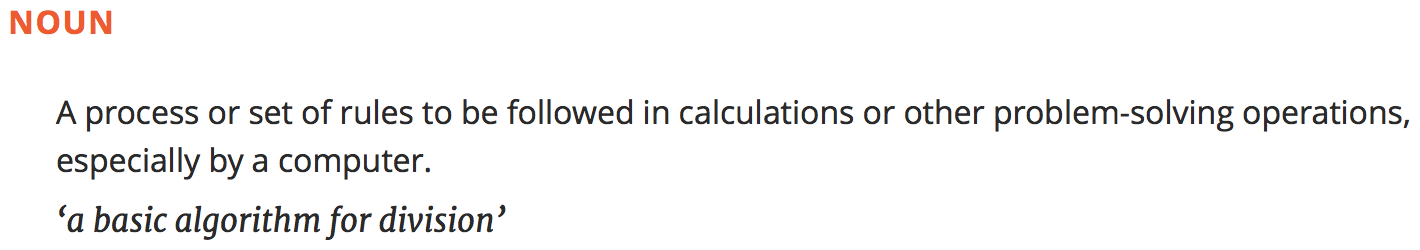
\includegraphics[scale=0.5]{algorithm}
\caption{Algorithm definition taken from the Oxford English Dictionary.}
\label{fig:algorithm}
\end{figure}

As we can see in Figure~\ref{fig:algorithm}, it is a ``process or set of rules'' followed when trying to solve a
problem. Even if it sounds easy in theory, reading lines of code and then understanding what steps are necessary for
a machine to perform to generate the expected output is rather complex and hard for a human being to
comprehend especially if the algorithm presented is complex. In a study conducted by Christopher D. Hundhausen et al.~\cite{av}, it was
proven that even though algorithm visualisation is not the ``perfect'' solution, it is definitely effective in teaching students and experienced developers how algorithms work.

There are many tools out there that already provide animations of algorithms, however one thing was a key factor in deciding
how to proceed with planning the whole software process: there are barely any standalone applications. Even though one
can find many websites which let people visualise algorithms' steps (e.g. a good example is VisuAlgo~\cite{visualgo}), this is not such a viable solution as the user cannot use the application whenever they want to, as an Internet connection is required.

Therefore, the plan was to create an app that can run offline and would feel natural to the user regardless of the operating system of choice. There are many Java implementations (i.e. resulting in jar executables), but one of the main drawbacks of using Java is the lack of proper GUI tools that can build native-feeling applications. As such, the decision was made to use the Electron framework~\cite{electron} originally built by the team behind the Atom text editor.
This framework uses only web tools to generate executables for the three main OS families (i.e. macOS, Windows and Linux) that provide the user with a native, modern and responsive feel.

The planning was made using the best agile practices~\cite{agile-methodologies}, eventually deciding on following a variation of XP programming. Designing an architectural plan was a major milestone to be reached as it took a considerable amount of time to be put in place. However, as discussed in future chapters, the implementation of the animation engine was a crucial and time consuming challenge that required the highest amount of effort.

The report also presents how the application was tested in various ways, as well as how it was evaluated using potential
end users. Finally, we shall discuss the roadmap of the project, the importance of the open source community
for Palgo as well as some final thoughts and lessons learned during the process.

\section{Aims}

The goals of the project were set and subsequently refined during many project meetings, as well as meeting with fellow classmates to get feedback along the way.

The main aims of the Algorithm Animator, however, have always been:
\begin{itemize}
	\item Create an efficient and easy-to-use animator.
	\item Make the animator a cross-platform application that would run natively on the main operating system families: macOS, Windows and Linux.
	\item Provide a user-friendly interface that would make the user enjoy using the product.
	\item Create at least 5-6 fully functional algorithm animations.
	\item Make the application scalable and easy to maintain.
	\item Test all functionality and ensure quality above quantity.
	\item Evaluate the product throughout the software process to meet acceptance criteria.
	\item Build a roadmap that would allow the animator to grow even after the level 4 project has finished.
\end{itemize}

\section{Motivation}

Even if we have previously mentioned that visualising algorithms is one of the best ways of understanding how they perform, there are also other key motivational aspects behind the need of building an animator.

One such motivation is the increasing demand of software engineers throughout industry as well as the rise in level of expertise. Developers, and students in particular, will benefit tremendously from a good grasp on how to implement correct and optimal algorithms when applying for a new job. Thus, an algorithm animator would be a good component in one's tool belt.

Another major aspect was the opportunity to create a modern application that users would enjoy using. At the
moment, one of the most popular animator toolkits is the one presented in John Morris' paper~\cite{animator-toolkit}.
Figure~\ref{fig:animator-toolkit} depicts a screenshot taken while using this toolkit. \newpage

\begin{figure}[!ht]
\centering
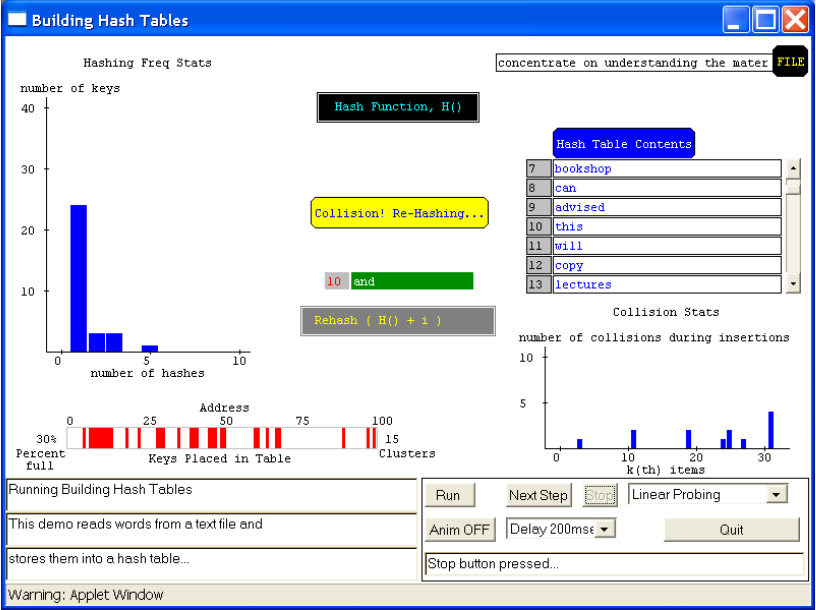
\includegraphics[scale=0.8]{animator-toolkit}
\caption{John Morris' Animator Toolkit.}
\label{fig:animator-toolkit}
\end{figure}

This toolkit was written in Java, which comes with certain advantages: multi-threading support, enhanced familiarity due to
university coursework and projects etc. However, the lack of proper graphical user interface components makes this a
not so viable option for regular users when adopting it. On the other hand, Figure~\ref{fig:palgo} shows our proposal to solve these shortcomings.

\begin{figure}[!ht]
\centering
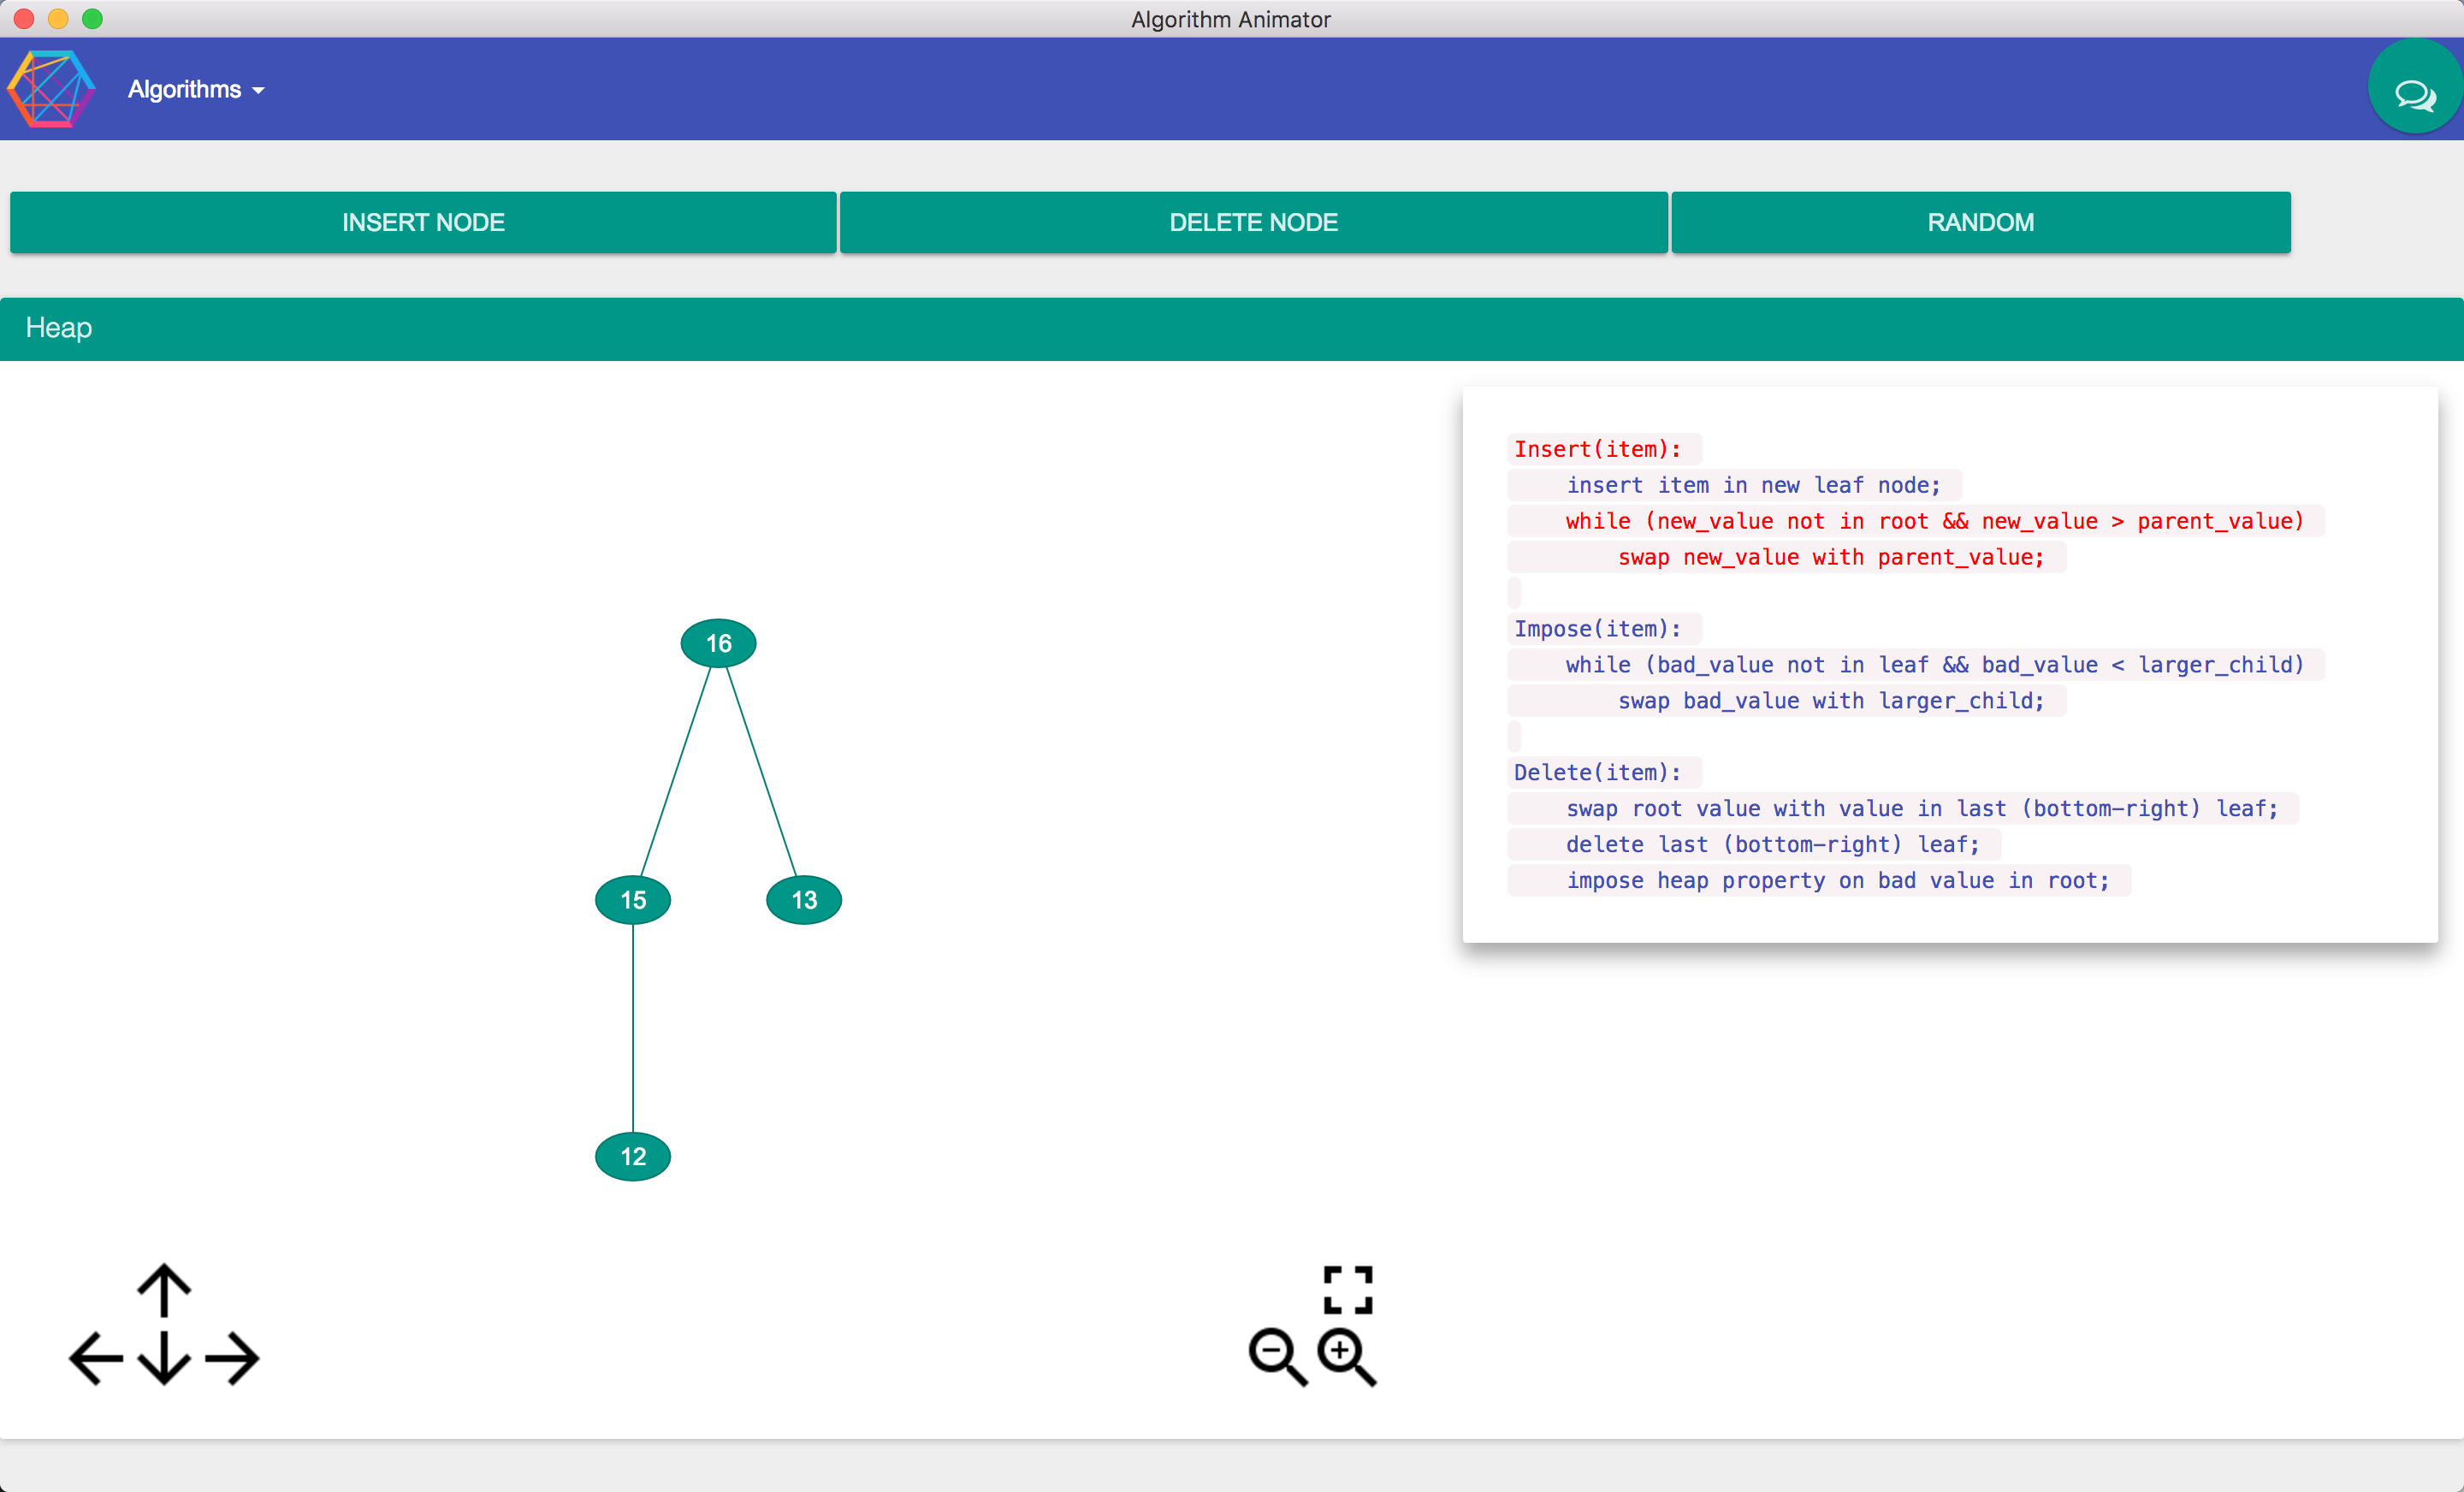
\includegraphics[scale=0.3]{algo-animator}
\caption{The animator presented in this report.}
\label{fig:palgo}
\end{figure}

We can see a clear difference between the two figures and why one might choose the latter option due to familiarity (native feel) and easy-to-use user interface.

\section{Contributions}

This report serves to deliver the following contributions.

\begin{itemize}
	\item Describe the whole software development lifecycle of an algorithm animator.
	\item Present the various technologies used to build native and modern desktop apps~\cite{electron}~\cite{visjs}
	\item Provide a brief overview of current animators available and background knowledge on their benefits and efficiency in teaching.
\end{itemize}


\section{Report Content}
The remainder of the report will analyse the background of animators and why they were proven useful, as well as cover all the steps in gathering requirements, designing, implementing, testing and evaluating the tool.

\begin{itemize}
\item Chapter~\ref{background} covers work related to the purpose of algorithm animators and why they are useful.
\item Chapter~\ref{requirements} goes into how the problem was analysed and what requirements were gathered through
	project meetings and discussions with Algorithmics students.
\item Chapter~\ref{agile-software-development} shows the steps undertaken to follow the best agile methodology principles.
\item Chapter~\ref{design} explains the design decisions behind the tool and illustrates various lessons learned and
	problems faced along the way.
\item Chapter~\ref{implementation} goes into the implementation details of the animator.
\item Chapter~\ref{testing} show how extensive unit, integration and other types of testing (e.g. smoke, end-to-end)
	were undergone and why they were essential to the development of the application.
\item Chapter~\ref{conclusions} details the overall results of the project.
\end{itemize}

%==============================================================================

\chapter{Background}
\label{background}

As stated in the introduction, the first step is to define what an algorithm is. We will use the above-mentioned definition taken from the Oxford
dictionary~\cite{oxford-dict}: ``A process or set of rules to be followed in calculations or other problem-solving operations, especially by a computer". In our case, we will only relate to set of rules followed solely by computers. Thus, put simply, an algorithm is a set of steps defined by someone in order to solve some problem. As an algorithm can be written by anyone, there is no known number or catalog of them. However, the most important algorithms (e.g. Huffman tree encoding/decoding) are taught in any Computer Science course at universities around the globe.

Having defined what an algorithm is, let's take an actual example - Dijkstra's algorithm for finding the shortest path
between two vertices of a graph~\cite{dijkstra-shortest-path}, first published almost 60 years ago (the pseudocode was formally
checked by Dr. Norman). Listing~\ref{dijkstra-pseudocode-snippet} presents the pseudocode for the algorithm.

\begin{lstlisting}[language={Java}, label={dijkstra-pseudocode-snippet}, caption={Pseudocode for Dijkstra's shortest
path algorithm.}]
// S is set of vertices for which shortest path from u is known
// d(w) represents length of a shortest path from u to w
// passing only through vertices of S
S = {u}; // initialise S
for (each vertex w) d(w) = wt(u,w); // initialise distances
while (S != V) { // still vertices to add to S find v not in S with d(v) minimum;
	add v to S;
	for (each w not in S) // perform relaxation
	d(w) = min{ d(w) , d(v)+wt(v,w) };
}
\end{lstlisting}

As one might observe, this is not trivial to grasp. Therefore, many solutions have been created in order to help
students and engineers in general understand them better. One such solution is a rather creative one, developed by
students at Spatienta University, which tries to teach different sorting algorithms by dancing
(Figure~\ref{fig:quicksort}).

\pagebreak

\begin{figure}[!ht]
\centering
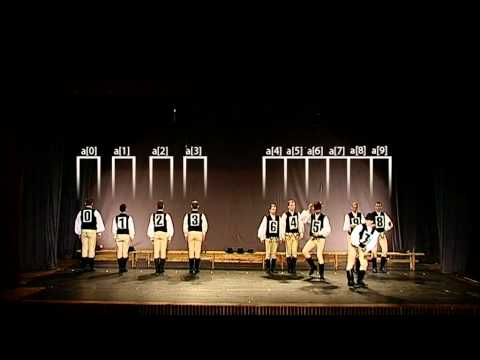
\includegraphics[scale=0.6]{quicksort}
\caption{Sorting algorithms learning through Hungarian folk dancing.}
\label{fig:quicksort}
\end{figure}

This was featured on many websites and gained enormous traction among computer science enthusiasts. However, a more
traditional approach that is adopted formally in universities as well is the use of animators and animation.

Firstly, let us define what an animator is. Again, taking the definition from the Oxford dictionary~\cite{oxford-dict},
it is ``a person who makes animated films". In our case, the person is the computer and the film is the sequence of steps required to produce an output after feeding input to an algorithm.

Usually, algorithm animators are divided into 2 sections: one section will contain the graphics in order to represent the
data structures used (e.g. in graph traversal algorithms the vertices and edges comprising the graph will be drawn) while
the other will have the code lines, the actual rules the computer needs to follow in order to produce the desired
output. The current code line that is executed at a certain moment is highlighted, while the data structure visualized
(e.g. some box that represents an array's element) changes and the user can see the output visually and immediately,
making a mental connection between the code line and the change it produces. Figure~\ref{fig:animation-panes} will present the two animation sections we have used in Palgo. 

\begin{figure}[!ht]
\centering
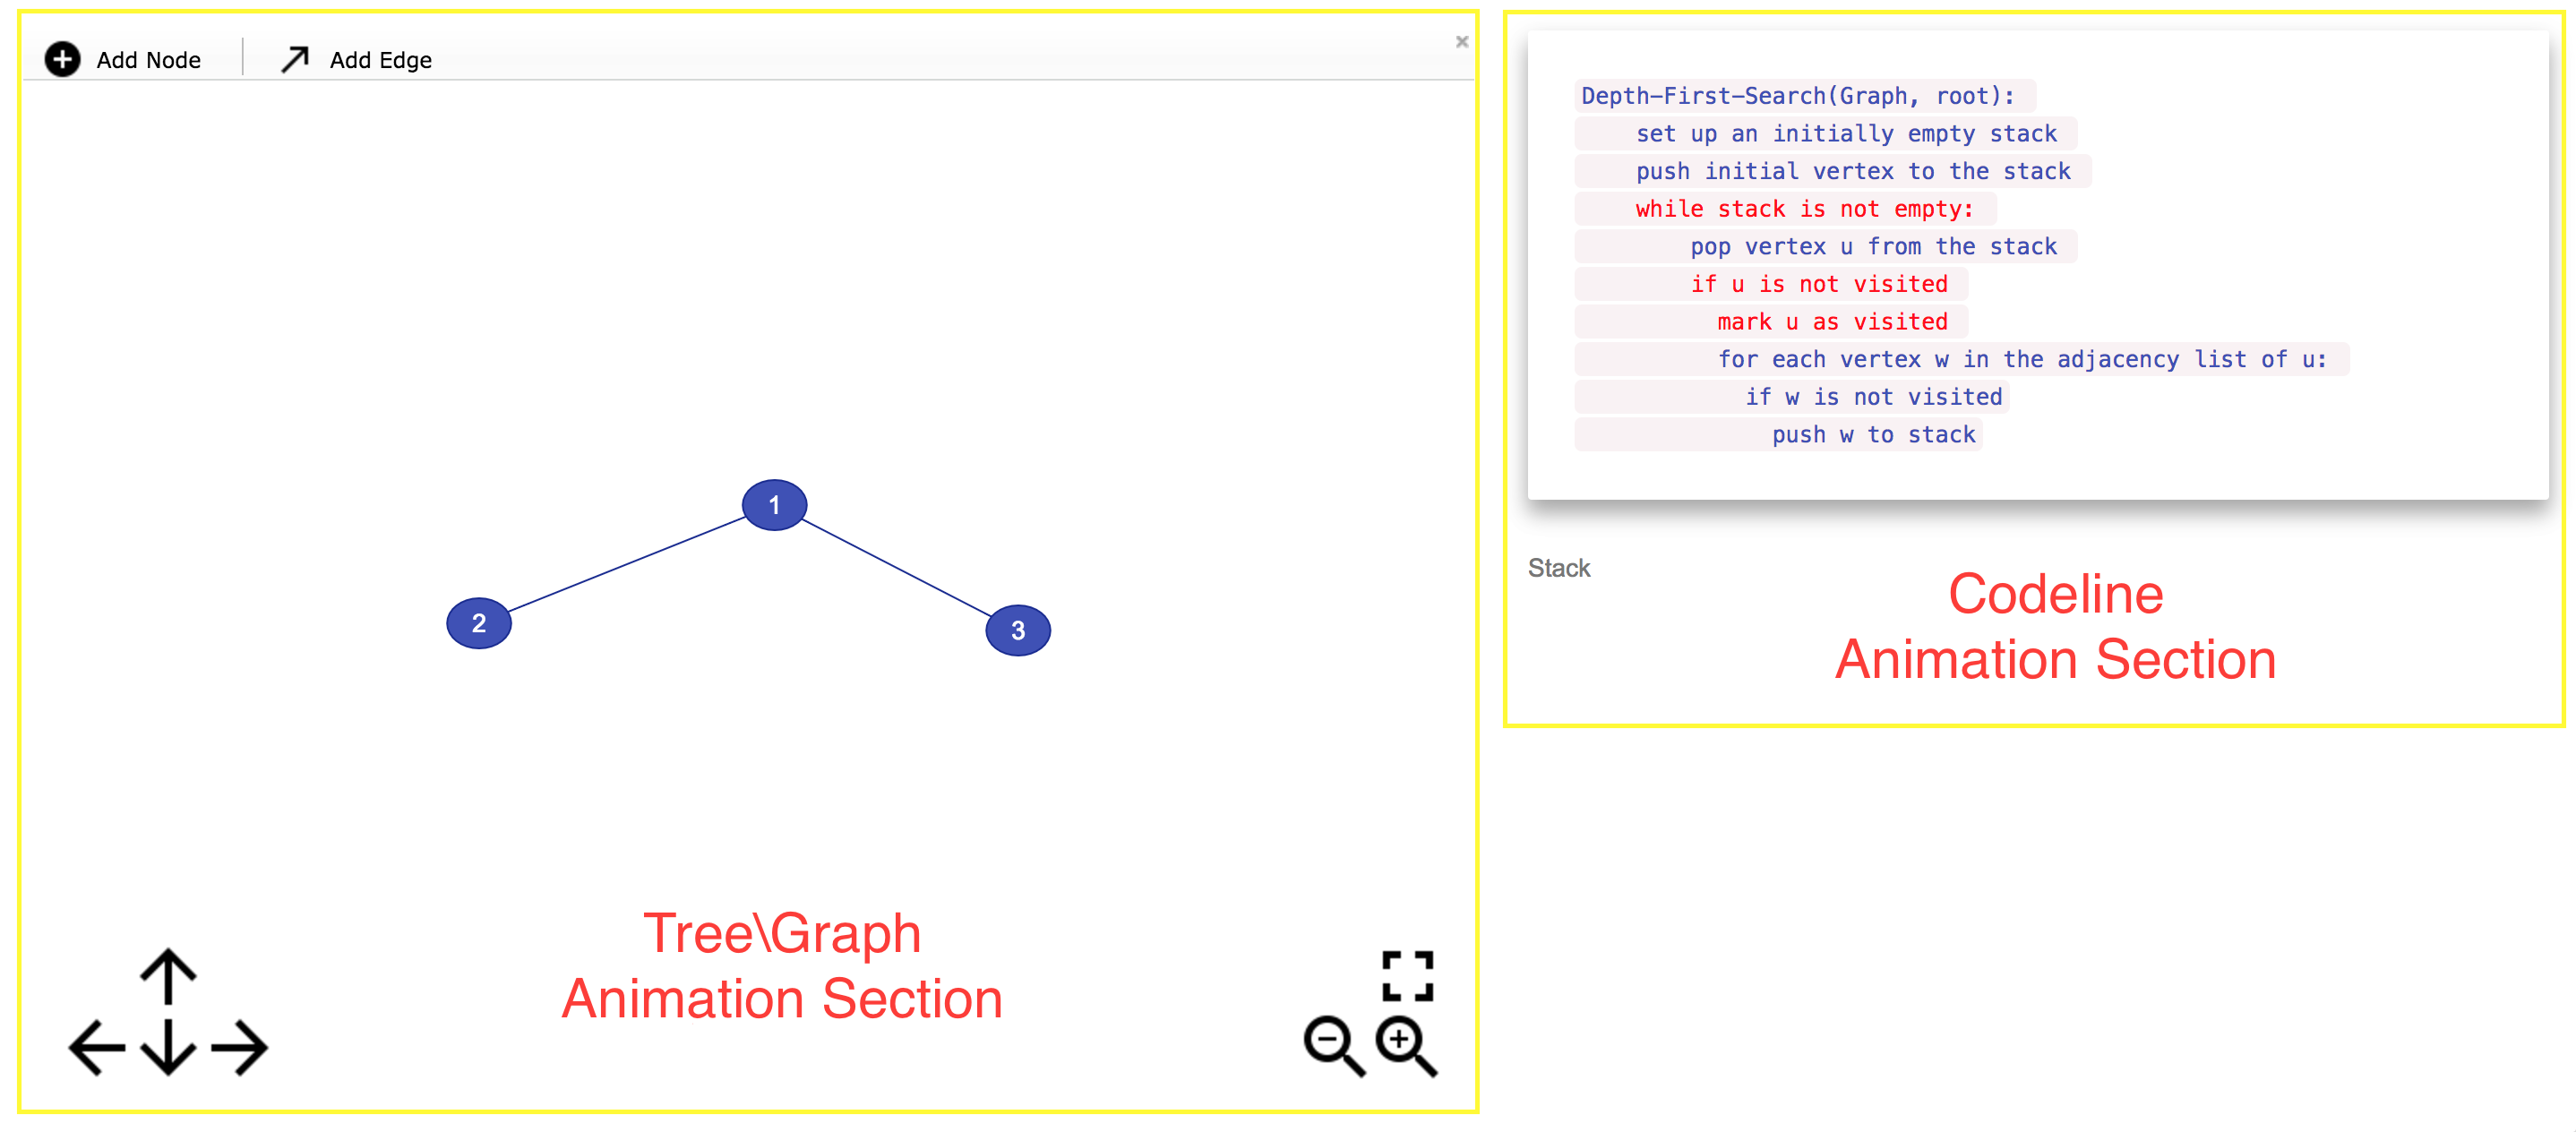
\includegraphics[scale=0.3]{animation-panes}
\caption{Sorting algorithms learning through Hungarian folk dancing.}
\label{fig:animation-panes}
\end{figure}

But why an animator precisely? There are many studies that show visualization in any area can enhance learning
capabilities drastically. Brenda Parker and Ian Mitchell's work~\cite{parker-mitchell} shows clearly how seeing the
steps can greatly improve a student's understanding of what is happening ``behind the scenes". On the other hand, even if animations were proven to be generally useful and beneficial for the learner, the study shows the need for visualising algorithms animated declines over time.

Another study by Susan Palmiter and Jay Elkerton~\cite{palmiter-elkerton} tried to find out which method was the most
effective in learning new computer-based tasks. Even though animations for complex mechanisms were found to be
ineffective when compared to animations for easier algorithms (e.g. parallel programming vs. graph traversal), they were shown to be very helpful
for understanding what is generally taught at university courses.

Having discussed methods of learning new algorithms better and why animators are useful, we need to take a look at
previous solutions developed. Apart from John Morris' tool shown in Figure~\ref{fig:animator-toolkit}, there are many other applications available, including Galant~\cite{galant} and the visualizer built by D. Galles~\cite{galles}.

\begin{figure}[!ht]
\centering
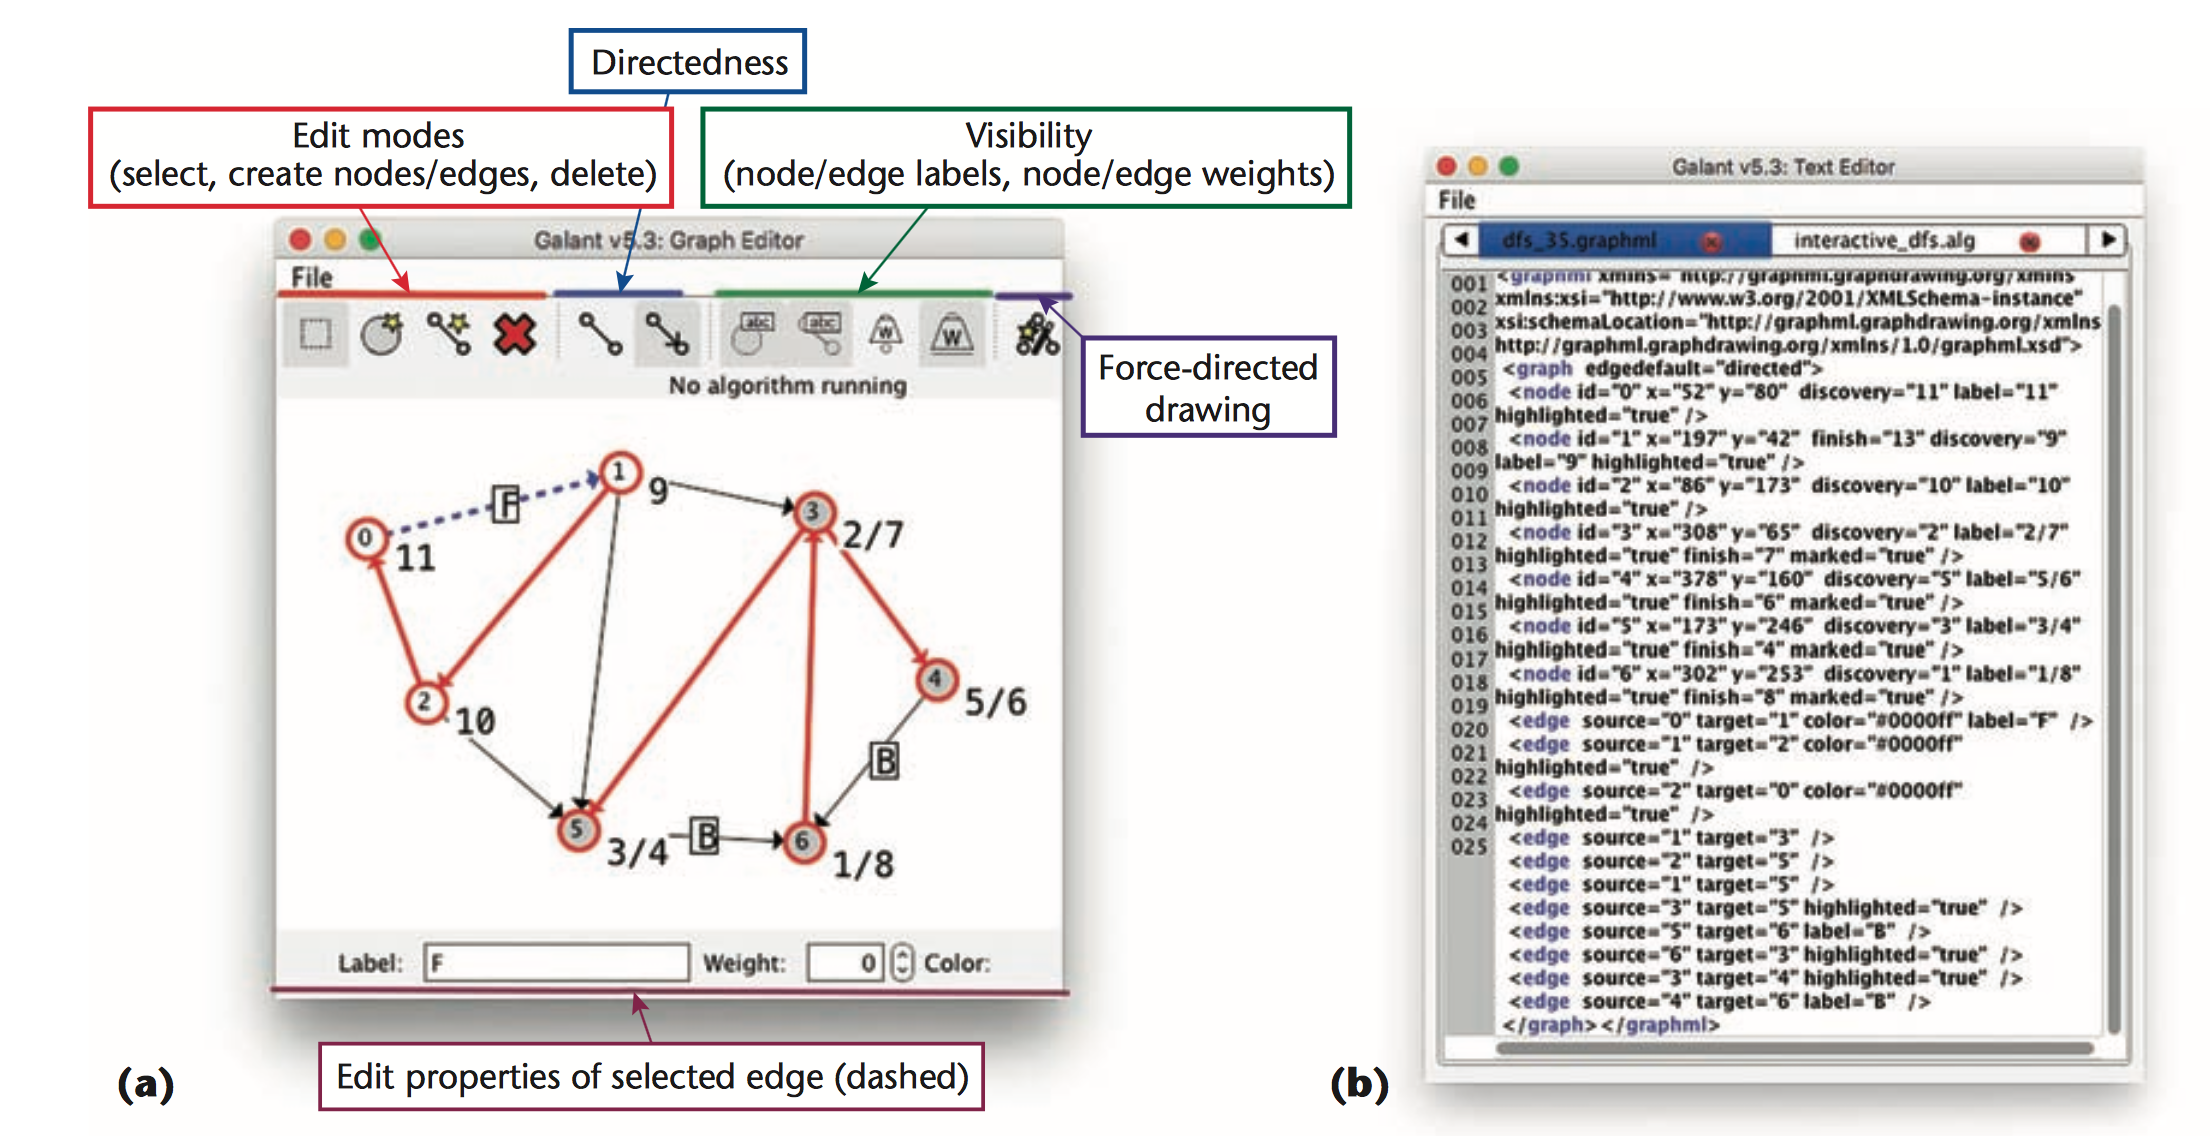
\includegraphics[scale=0.4]{galant}
\caption{Galant Algorithm Animator.}
\label{fig:galant}
\end{figure}

In Figure~\ref{fig:galant} we can see one of the two main approaches for building an animator, which is a standalone JAR application. Thus, it is written completely in Java and, as the language is pre-installed on most electronic devices, it can run on the major operating systems.

There are obvious advantages to this approach:
\begin{itemize}
	\item the end product can run on a variety of machines with only one codebase;
	\item the large number of Java libraries facilitate an easy development workflow;
    \item there are many tutorials and resources available;
    \item Java is taught at most universities, making it easier for newcomers to create their
      own application rapidly; Figure~\ref{fig:java-uni} shows what programming languages are preferred for teaching in
      introductory courses at prestigious Computer Science departments in the U.S.

\begin{figure}[!ht]
\centering
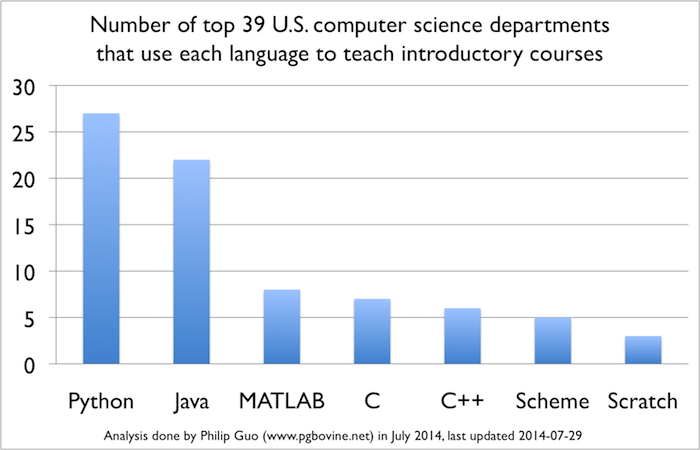
\includegraphics[scale=0.8]{java-uni}
\caption{Languages used in introductory courses at top US universities.}
\label{fig:java-uni}
\end{figure}
\end{itemize}

\pagebreak

However, there are also drawbacks to creating a standalone JAR application:
\begin{itemize}
\item the most popular Java libraries for producing standalone graphical JAR applications output old-fashioned user
  interface;
\item the code for drawing on the canvas and animating in Java (using Swing or JavaFX) can become extremely verbose
  and unreadable.
\end{itemize}

The second main approach for building an animator is web-based, one of them being D. Galles'
application~\cite{galles}. Figure~\ref{fig:galles} shows a screenshot taken while using this application.

\begin{figure}[!ht]
\centering
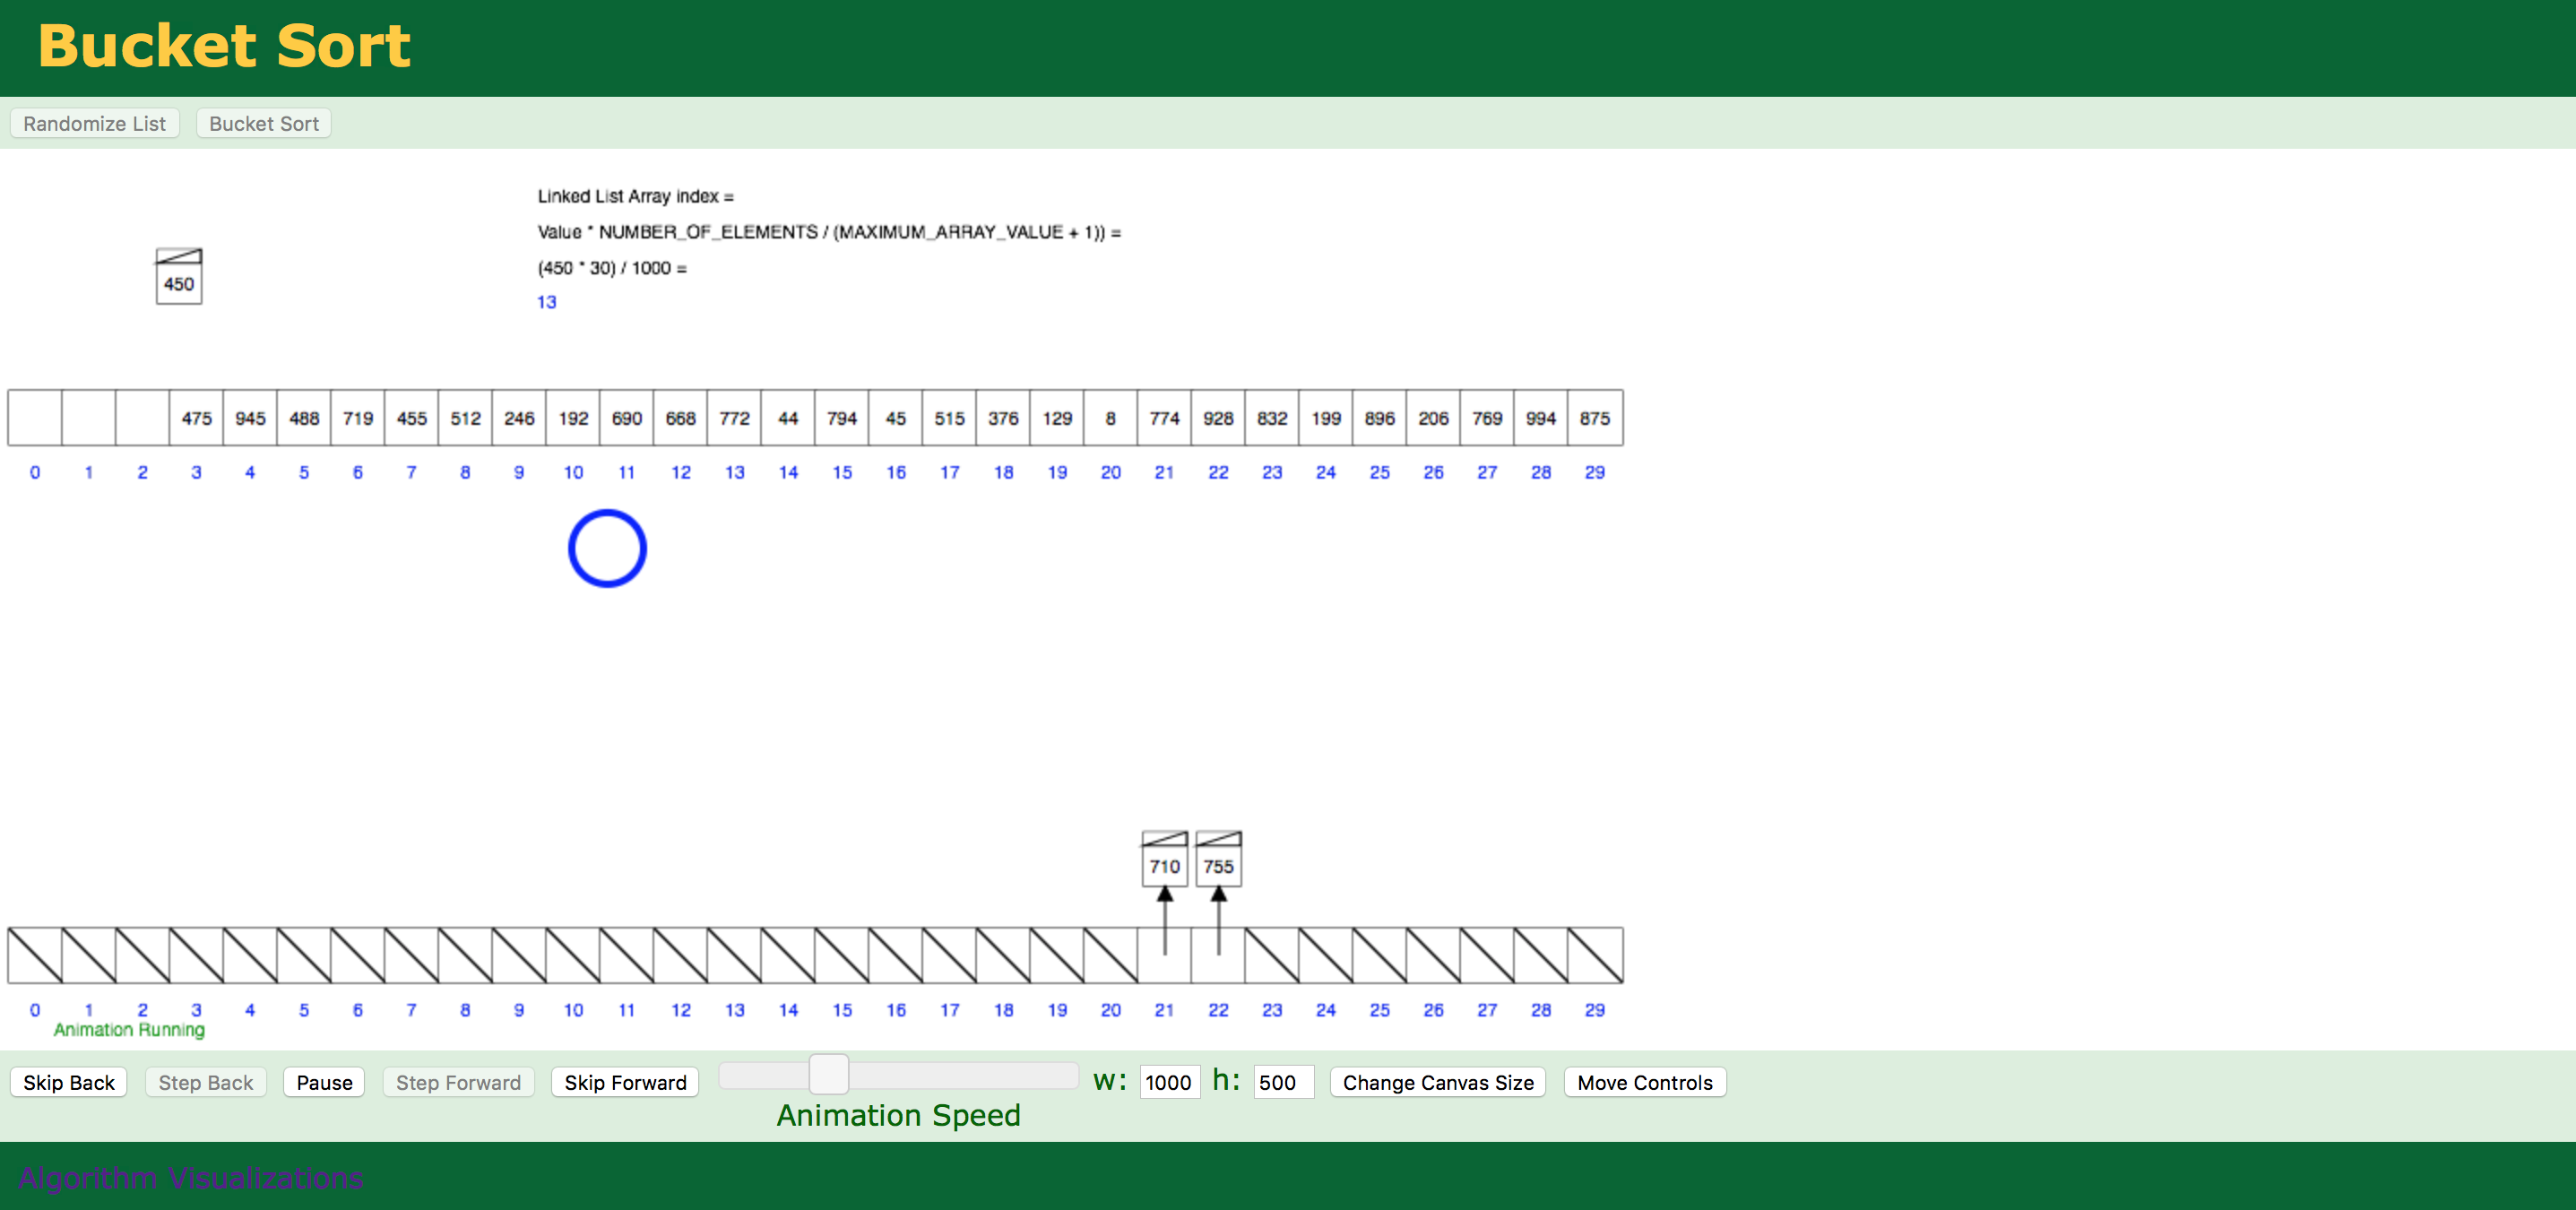
\includegraphics[scale=0.25]{galles}
\caption{Algorithm animator built by D. Galles at University of San Francisco.}
\label{fig:galles}
\end{figure}

The main advantages of a web-based approach are  that:
\begin{itemize}
\item the developer can use a wide variety of JavaScript tools (e.g. drawing directly on HTML5 canvas, VisJs and SigmaJs)
  to draw and animate objects;
\item the application can have a very moxdern and responsive feel which can enhance users enjoyment the product;
\item virtually all users have at least a browser installed on their machine, thus making the animator available to
  everyone.
\end{itemize}

However, the main drawback is that it is still a website, thus it need to be hosted (which implies additional costs) and it cannot be reached by everyone at all times due to the fact that not everyone has constant internet access.

We have covered all the necessary background and related work before diving into how Palgo was designed and implemented. We believe that our solution is a combination of the two main approaches listed above, merging the benefits of both into a single tool.

%==============================================================================

\chapter{Requirements}
\label{requirements}

As for all other software built with best practices, requirements need to be gathered, defined, analyzed and then prioritized. As we tried to follow an Agile structure, the requirements changed every week through student-supervisor weekly meetings, as well as end user meet-ups.

We tried to keep the requirements SMART~\cite{smart-requirements}, which implies they are specific, measurable,
attainable, realizable and time bounded. Making the requirements follow this well established format made the software development lifecycle much faster and cleaner.

Figure~\ref{fig:trello-functional-requirements} shows a screenshot from a Trello~\cite{trello} board used during one of the iterations (a separate board was used for tracking non-functional requirements as well).

\begin{figure}[!ht]
\centering
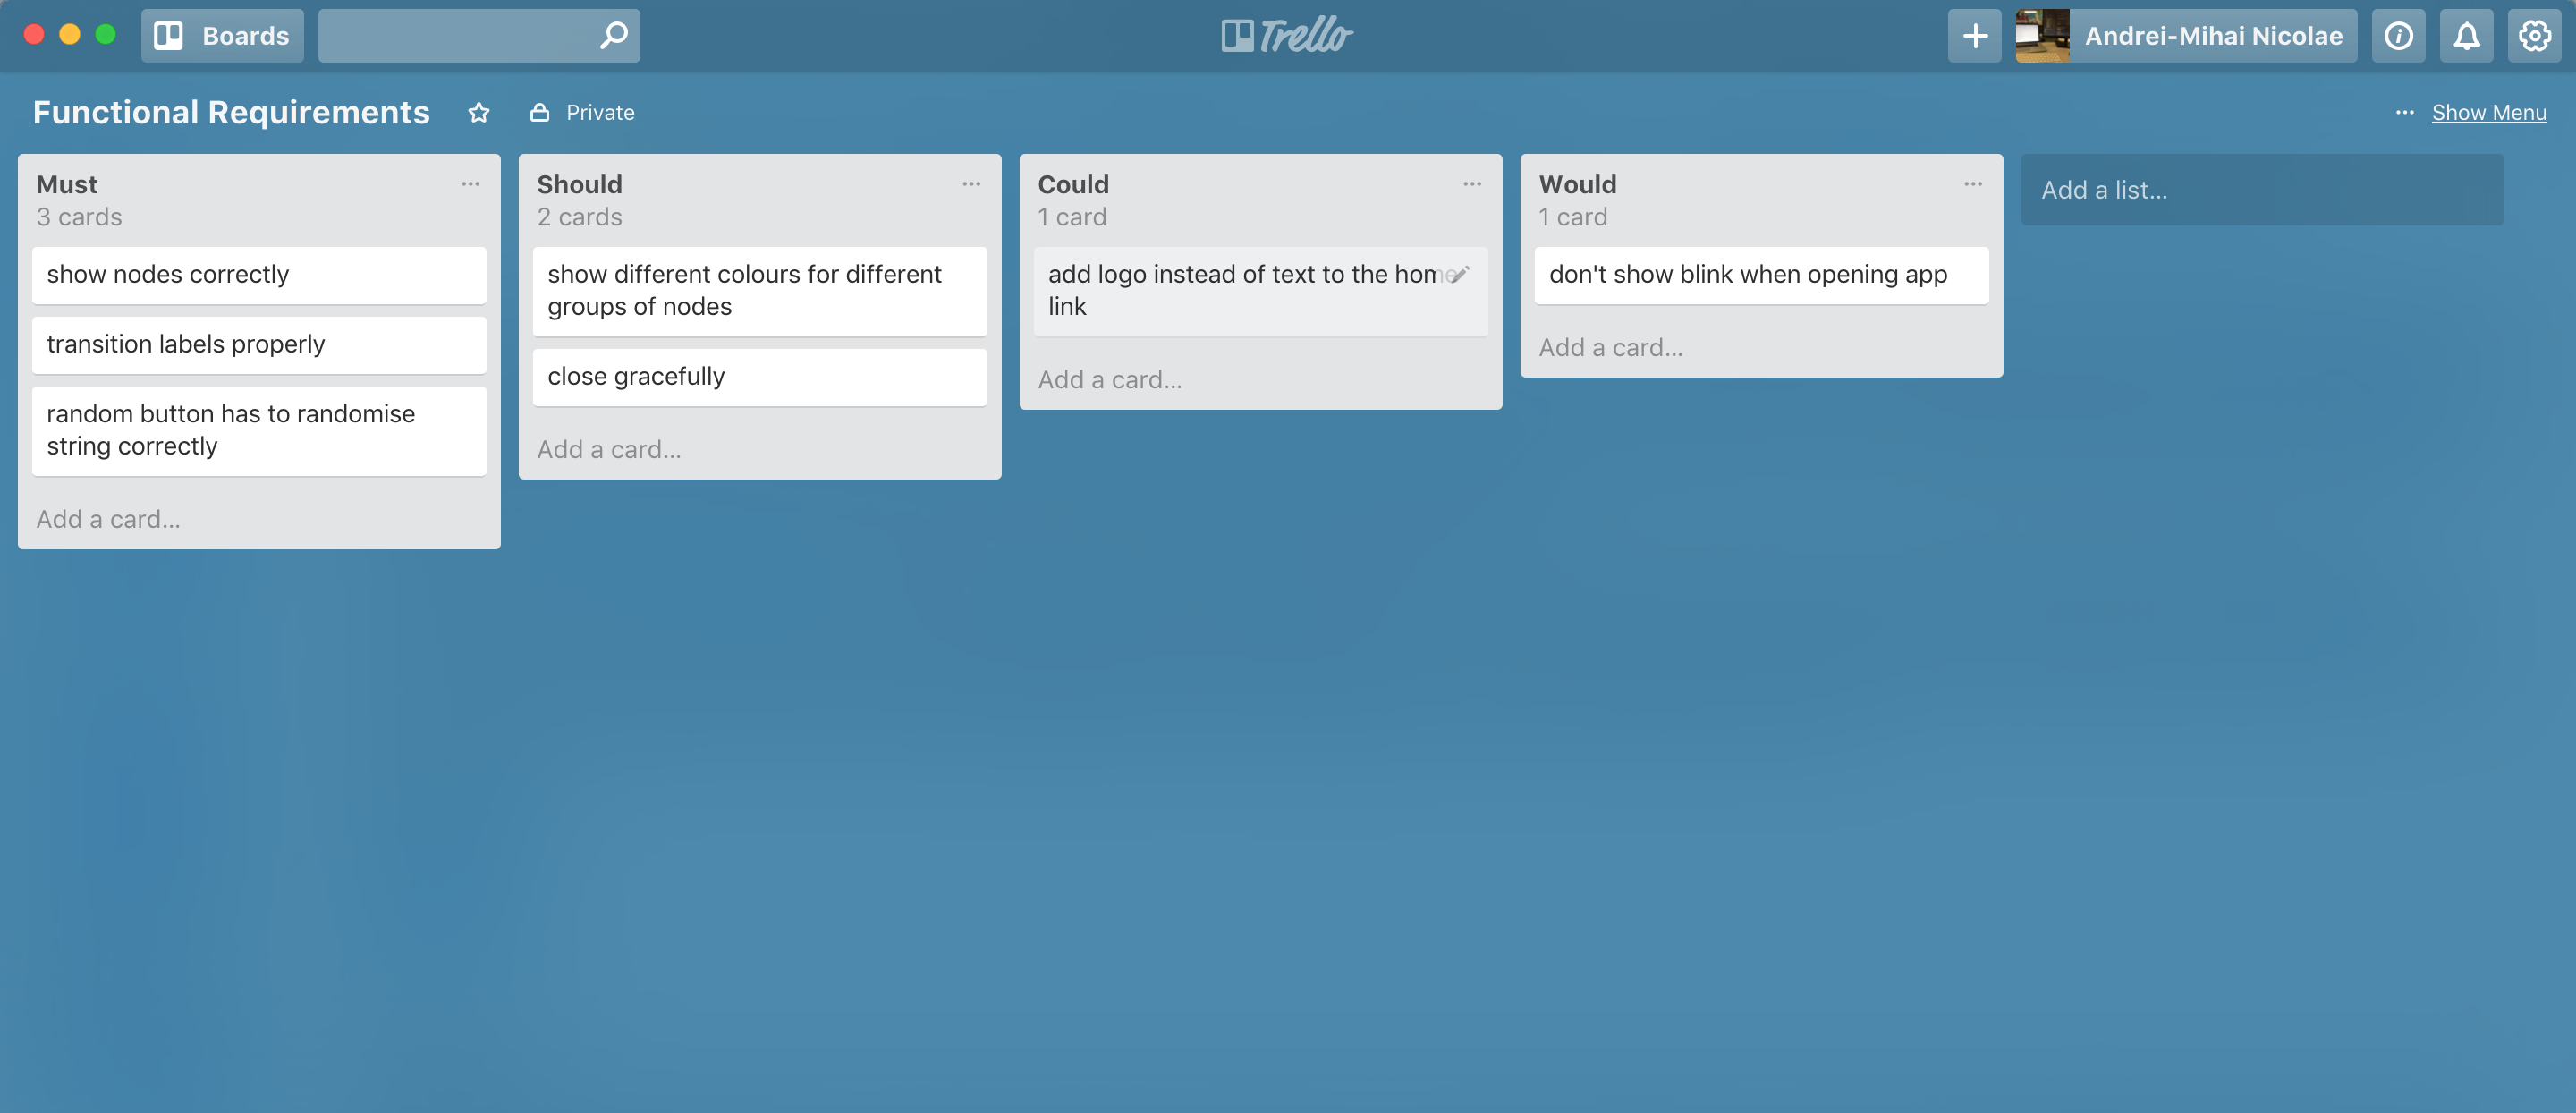
\includegraphics[scale=0.35]{trello-functional-requirements}
\caption{Trello board for functional requirements during one of the iterations.}
\label{fig:trello-functional-requirements}
\end{figure}

The requirements followed a pipeline through which they, together with their rationale, would get broken down
into pieces continuously until user stories could be produced. One example of such a requirement is: ``Show me a
correct and easy-to-understand animation for the insert function in a heap data structure.''. This would then be broken
down in multiple user stories, such as ``Colour the node that is inserted and add its label" and ``Highlight code line corresponding with changing the label".

We also tried to follow the MoSCoW~\cite{moscow-requirements} guideline for prioritizing the requirements. The technique has proven to be very effective and it is adopted widely in industry, even though the approach is more than 20 years old. This facilitated a smooth workflow and concise goals to be targeted.

\section{Problem Analysis}

We have analyzed the problem systematically, dividing it into the following main questions:

\begin{itemize}
\item who are our target users?
\item what type of format will the application have (i.e. web/desktop)?
\item what algorithms should be animated?
\item how would the main layout be structured?
\end{itemize}

During the analysis, we needed to take into account various factors, including how much experience with algorithms and
computer science in general will our users have and what algorithms would need visualization the most. As previous animators built under the supervision of Dr. Norman are used for educational purposes in the level 3 Algorithmics I course, we believe that having mainly graph and tree algorithms would benefit the project the most. However, we tried to keep the structure simple and the codebase easy-to-maintain so that other families of algorithms will be straightforward to implement. Because we want to project to be continued in the open source space, users other than students can use the animator, thus we tried to keep the requirements more general.

Also, there was much discussion around whether to use a web or a desktop approach. For reasons explained above, we
decided to implement a desktop application using the technologies mentioned in the subsequent chapters.

We have gathered the requirements and split them into functional and non-functional, then dividing them further into
smaller tasks to be implemented. In the end, we were left with user stories that could be translated directly into work tasks.

\section{Requirements Gathering}

As mentioned above, the requirements gathering was a continuous process that lasted from the first week of 4th year up until the end of the project's development lifecycle. Not only were there the regular weekly student-supervisor meetings where we could add or refine requirements, but there were also meetings with possible end users. More precisely, every two or three weeks there were meetings scheduled with a few classmates from University of Glasgow's Computer Science course that would give continuous feedback after testing the newest version of the application. The meetings were held in one of the laboratories in the Boyd Orr building where the classmates were provided with an executable that could be run on their personal laptops. They were given around 15 minutes to try the features and, afterwards, they provided invaluable feedback without which the animator would not perform as efficiently as it does today.

\section{Functional Requirements}

Functional requirements target specific functionalities that the system should perform. They started with the algorithms that needed to be animated. Then, functionalities such as current code line highlighting and specific button behaviors began to stack up. Eventually, we can categorize them as follows:

\begin{itemize}
\item animate tree/graph depending on what the user chose to do (e.g.\ insert/delete node);
\item highlight current code line for every algorithm;
\item define specific behavior for every button displayed on the UI;
\item each window interaction should perform as expected depending on the operating system the user is using the
  application on;
\end{itemize}

Many smaller functional requirements appeared along the software process, but the above mentioned are the main categories.

\section{Non-Functional Requirements}

A non-functional requirement is a type of requirements that judges the system as a whole and how it operates rather than checking for specific criteria. The main non-functional requirements were rather set from the beginning. We decided to have an algorithm animator that would:

\begin{itemize}
\item be easy to use and let the users familiarize rapidly;
\item make users enjoy playing with the product;
\item be installed/fetched with ease;
\item allow end users to use it on any platform;
\item be efficient and not consume excessive resources;
\item be maintainable and scalable (i.e.\ let future possible contributors add algorithms easily).
\end{itemize}

%==============================================================================

\chapter{Agile Software Development}
\label{agile-software-development}

Good software practices are key to successful projects. We have followed Agile methodologies, in particular, the methodogies that were taught last year in the Professional Software Development class, as well as through Ian Sommerville's ``Software
Engineering'' book~\cite{software-engineering}.

We eventually decided to follow an Extreme Programming path and we implemented the best advice taken from industry
experts. Some of the key principles we implemented throughout the whole process are:
\begin{itemize}
    \item good planning strategy that would allow us to follow a schedule; our cost estimation efficiency improved
      with every iteration;
    \item frequent commits and releases that would generate continuous feedback from our potential end users;
    \item customer involvement (i.e. student meetings every few weeks as well as weekly student-supervisor
      meetings);
    \item heavy refactoring as opportunity arose;
    \item emphasis on simplicity in design and implementation;
    \item tracking bugs and issues in general allowed us to be always informed and include necessary items for
      specific milestones so that the quality would always have high standards.
\end{itemize}

These principles ensured a good workflow with promising results that were immediately noticed. We believe that a major part of the
success of the project was embracing above Agile methodologies.

\section{Extreme Programming}

We have followed the approach first coined by Kent Beck called Extreme Programming (XP)~\cite{extreme-programming}. It is an
Agile technique through which good practices are pushed to ``extreme'' levels. XP has proven to be very effective as many companies use it in their development lifecycle. Principles it promotes that we have followed include:

\begin{itemize}
\item frequent releases based on requirements gathered incrementally in meetings (e.g.\ supervisor-student meetings)
\item constant refactoring to promote simplicity;
\item customer involvement throughout the whole process (i.e.\ getting feedback every 2-3 weeks from students that might use the application);
\item people over processes, which means collective ownership of the code as well as avoiding exhausting long working hours.
\end{itemize}

Burndown charts are another great tool used by developers using XP in their schedule to track progress. You start off by defining the number of user stories you want to complete in an iteration and, then, divide that number by the number of days the sprint has (in our case it was 7 days). Therefore each day you should implement a certain number of user stories such that at the end of the iteration you are left with none. That is the most productive outcome. Also, because this was a student project, we will count weekend days as working days.

During the entire process we tried to monitor the progress and see how we are performing.
Figure~\ref{fig:burndown-november} shows a burndown chart from one of the November weekly iterations.

\begin{figure}[!ht]
\centering
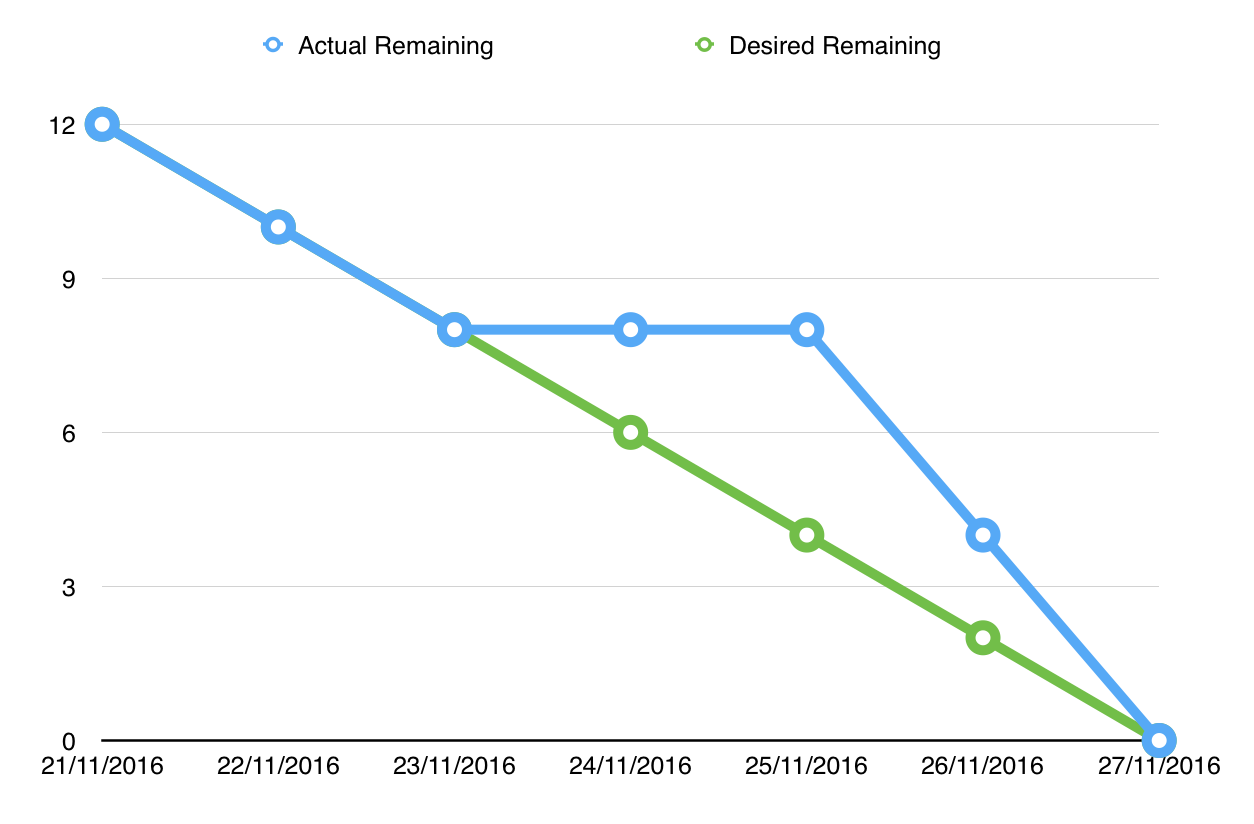
\includegraphics[scale=0.6]{burndown}
\caption{November iteration burndown chart.}
\label{fig:burndown-november}
\end{figure}

As one can notice, there is quite a discrepancy between the desired number of user stories per day and what we actually
completed. This was because of lack of consistency, shown in the graph between days 23 and 26, where there were no user
stories finished. However, Figure~\ref{fig:burndown-february} depicts a burndown chart corresponding to one of the last iterations of the project.

\pagebreak

\begin{figure}[!ht]
\centering
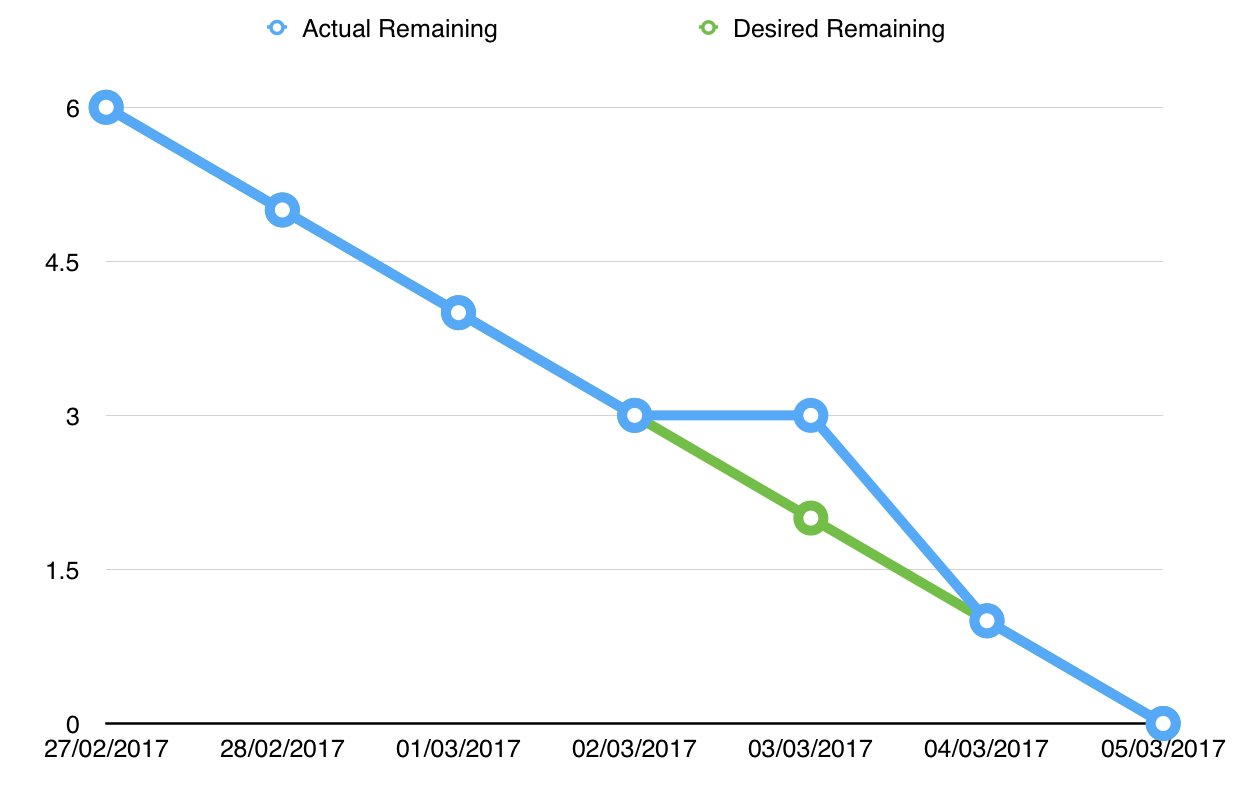
\includegraphics[scale=0.6]{recent-burndown}
\caption{February-March iteration burndown chart.}
\label{fig:burndown-february}
\end{figure}

There are noticeable difference between the 2 iterations: firstly, we started with fewer user stories to be completed in the latter sprint which was much more feasible to finish and it did not make us work extra hours (like in the first burndown chart example), thus violating one of the extreme programing principles. Moreover, there was only a slight discrepancy from the schedule on March 3rd where there were no user stories completed. However, this is relatively minor and we believe that for a two people project, this was an amazing achievement that could only be reached gradually.

Summing up, following all the good practices of XP has brought us great benefits and a working schedule that allowed us to implement all the requirements gathered in user and supervisor meetings.

\section{Planning}

Planning is a vital part of every Agile project - it involves setting deadlines for tasks needed to be implemented by
developers. However, as some tasks are not trivial to estimate, multiple strategies have been invented so that team
members can effectively set number of days (or other units of work) for every user story.

In our case we adapted the most effective Agile method, which is
Planning Poker~\cite{planning-poker}. In this practice, all developers are given decks of cards and when a user story is brought up, every developer shows a card which has a value. That value will represent the number of units of work
needed to complete the story. Then, after everyone shows their estimation, discussions emerge among the developers until a consensus is reached. In our situation, we did not use a deck of cards during the student-supervisor meetings, but we both estimated the number of days needed to implement a feature and, if our opinions diverged, we discussed until we had the same duration in mind.

It can be observed in Figure~\ref{fig:estimation} how we kept track of all the user stories using Trello cards. We added the estimation in the
description, as well as a description using the popular format ``As a $\dots$/I want to $\dots$/So that $\dots$"~\cite{user-story-format} to always know the
rationale behind every implemented feature.

\pagebreak

\begin{figure}[!ht]
\centering
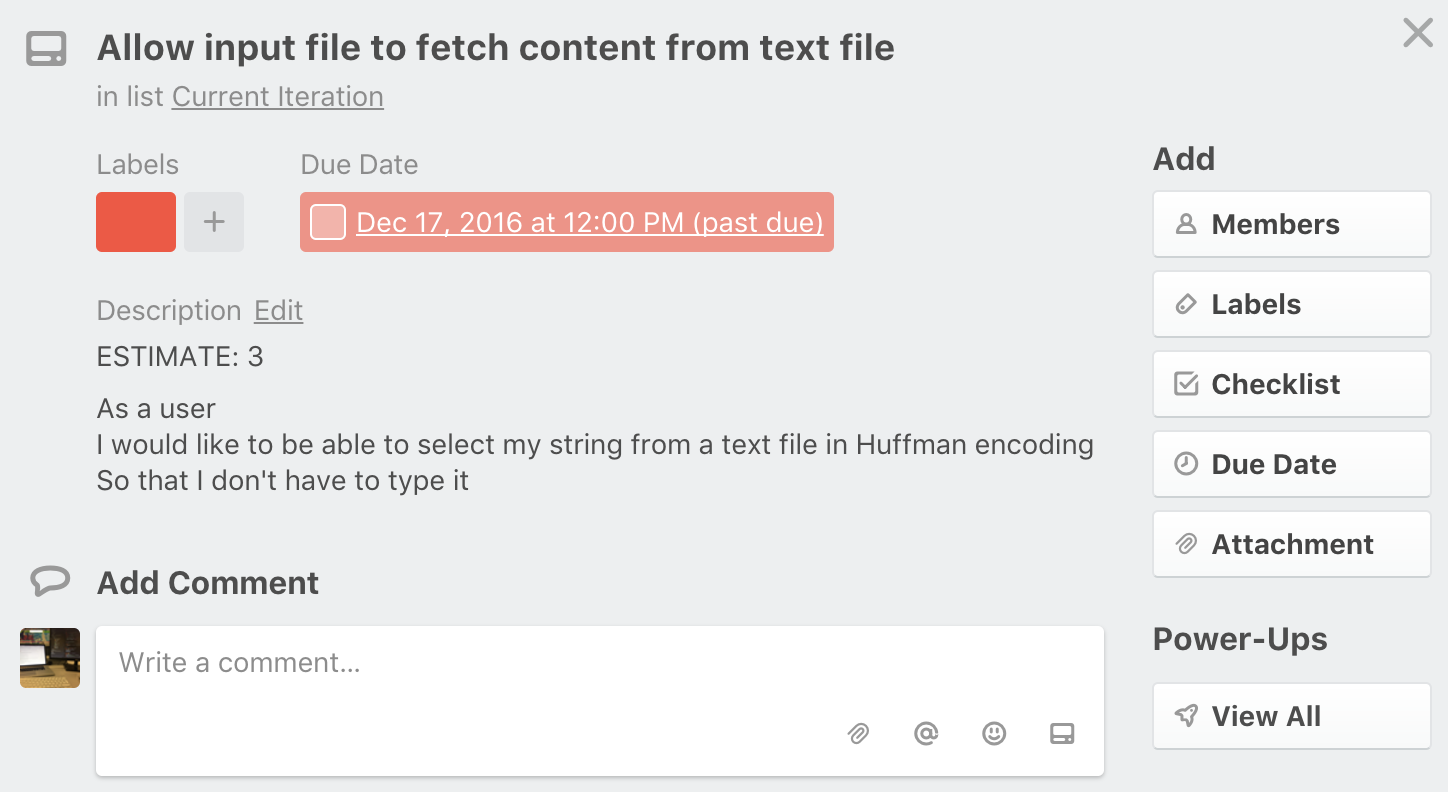
\includegraphics[scale=0.5]{estimation}
\caption{Trello card for estimating a user story.}
\label{fig:estimation}
\end{figure}

This method was very effective and as we gained more experience after several iterations, we would come to a conclusion
much faster and the user story cost estimations became more accurate.

\section{Continuous Integration}

We have used another tool heavily promoted by Agile methodologies which is Continuous Integration (CI). CI means
merging all working copies of everyone who is developing on the project to a shared mainline multiple times a
day~\cite{continuous-integration}. This is a very useful tool for checking that the builds do not break regardless of the
changes made and that quality is of primary importance.

In our case, we have used CircleCI~\cite{circleci} as the tool for CI. It was configured such that after every
commit, the code would be merged into the main branch, tested to see it everything is working as expected and, only
after, the code would be pushed.

\begin{figure}[!ht]
    \centering
    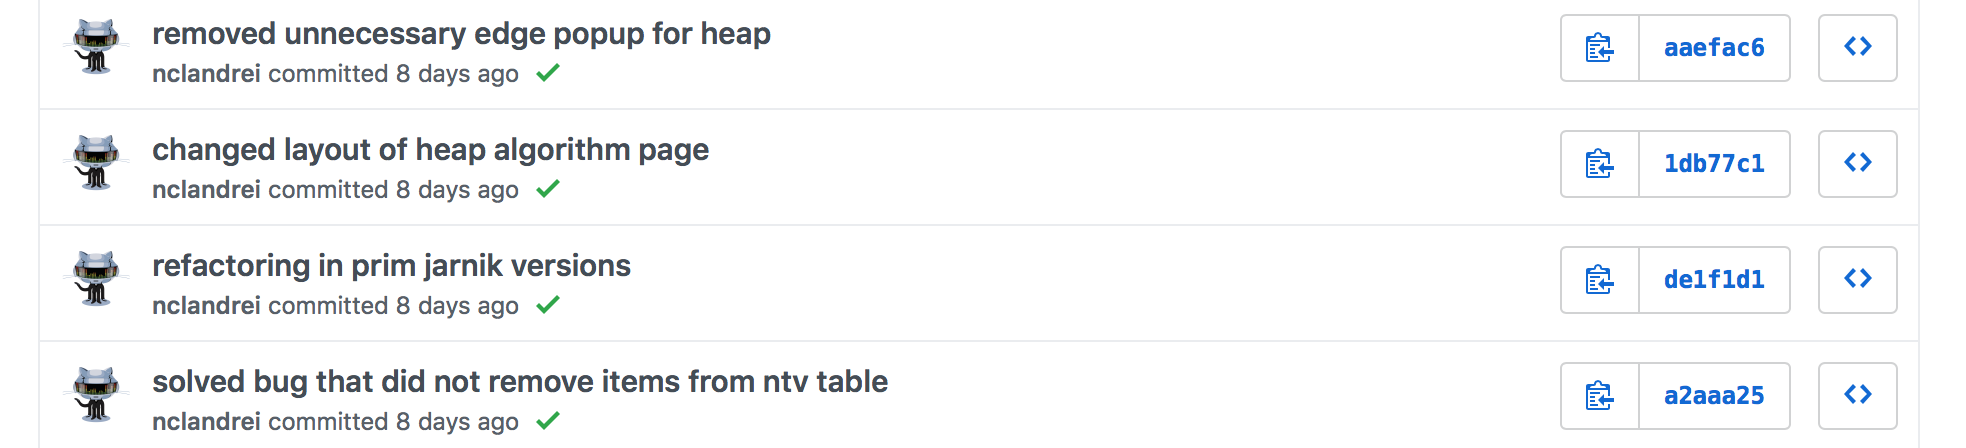
\includegraphics[scale=0.5]{circleci}
    \caption{CircleCI status showing red/green depending if the build was successful on GitHub.}
    \label{fig:circleci}
\end{figure}

As it can be seen in Figure~\ref{fig:circleci}, there is a small green check on the GitHub repository
of the project telling the developers that the build worked as expected (there would be a red cross in cases when the build did not work as expected). This was a great asset to the development lifecycle,
informing us whether we needed to add bugs to our tracking system to be solved later or if everything performed
exactly as it should have.

Not only did we applied continuous integration to our workflow, but we also used it properly: as
mentioned above, the definition of CI means the developers should push their local changes to the main repository
multiple times a day. Every day of development meant multiple commits and multiple pushes so that we made sure the
builds were all passing and the code was not broken.

\begin{figure}[!ht]
    \centering
    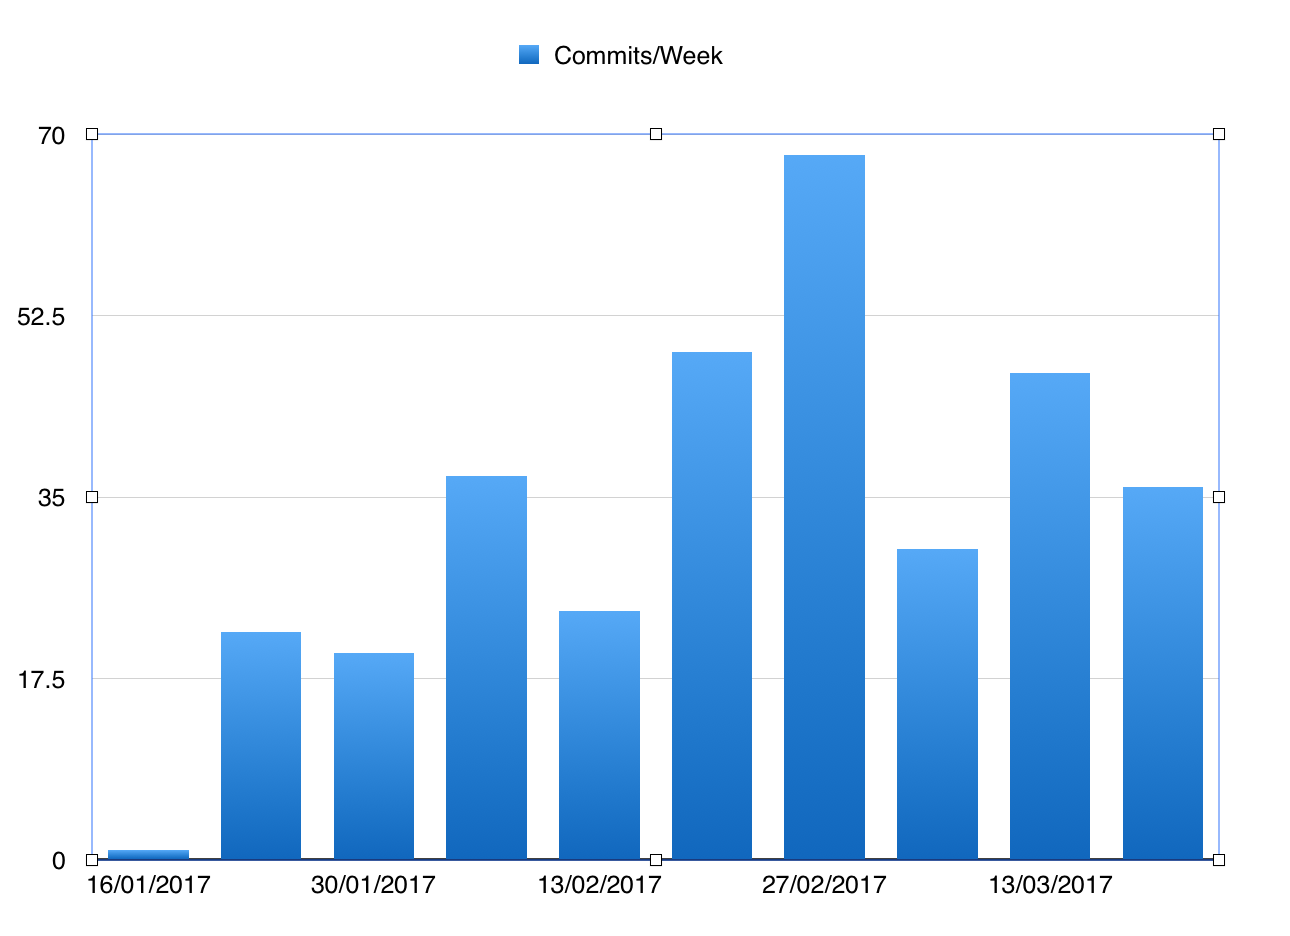
\includegraphics[scale=0.5]{commits-week}
    \caption{Commit frequency in the last 10 sprints.}
    \label{fig:commits-week}
\end{figure}

Figure~\ref{fig:commits-week} shows the commit frequency per week for the last 10 iterations. As it can be observed, apart from first week which corresponds with the first week of the University semester, the number of commits was very high for every sprint, thus following the practice of
committing and testing the quality of our product often.

\section{Issues \& Bug Tracking}

Issues and bugs occur all the time in every piece of software. Because the userbase was rather limited, I updated the
database manually from what we (i.e. Dr. Norman and myself) found not working as expected and what the students marked as
functionality not working properly or wanted features. This was a very useful practice to follow because it also
promoted continuous feedback on changes from potential end users, thus implementing the Agile manifesto properly.

Talking about actual implementation, we have kept a custom database on GitHub in order to be always up-to-date with what
is going on and allow us to spot where we lack quality and efficiency. We have made use of the custom labels GitHub already provides,
among which the most used ones have been:

\begin{itemize}
    \item \emph{bug} -- here we marked flaws in the system (or the students who have been providing constant feedback);
    \item \emph{enhancement} -- we added here the features most wanted by our users or by ourselves; this was refined from the
	requirements gatherings previously mentioned that ended up as multiple user stories eventually;
    \item \emph{question} - -these were marked for research purposes - one example might be: can we change the shape of vertices of a graph dynamically as the algorithm animation makes progress?
\end{itemize}

As an example, Figure~\ref{fig:issue-tracking} shows how issues were continuously tracked throughout the software process.
This screenshot was taken during one of the iterations.

\begin{figure}[!ht]
    \centering
    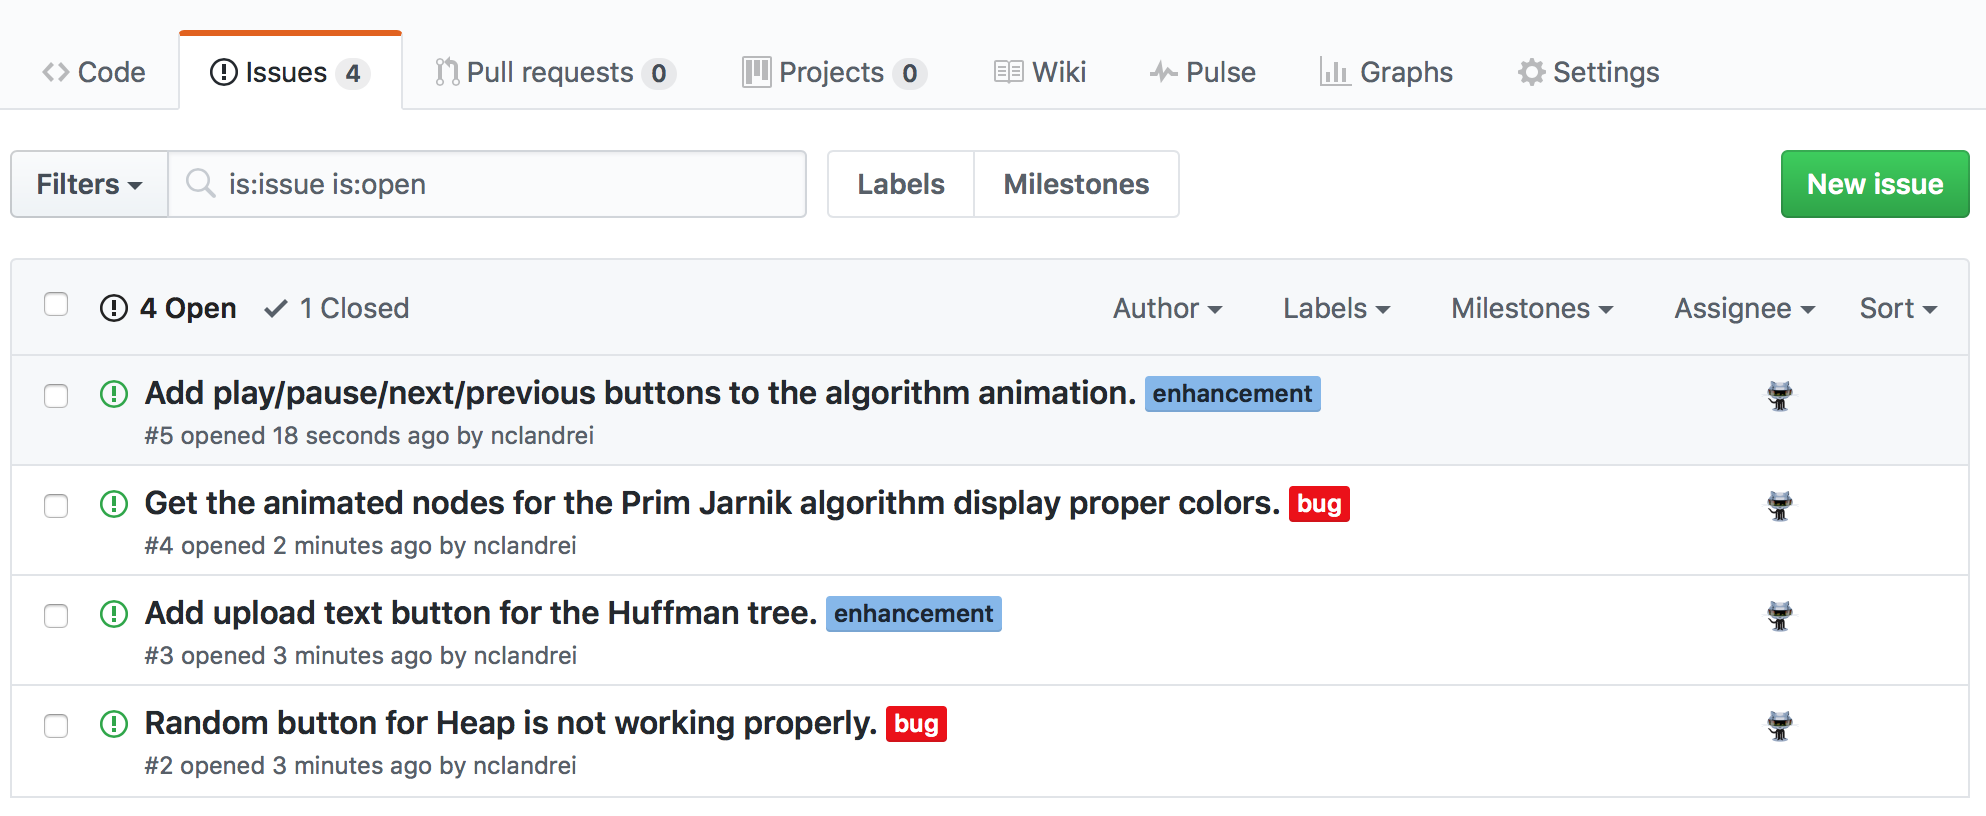
\includegraphics[scale=0.5]{issue-tracking}
    \caption{Example of issue and bug tracking in the GitHub provided Issues page.}
    \label{fig:issue-tracking}
\end{figure}

As it can be seen in the figure, there is also a milestone tab assigned to each issue. Because the screenshot is
from an earlier sprint, there were not milestones attached, but since January every issue had one so that we
would plan effectively and reach all goals by the negotiated deadline.

%==============================================================================

\chapter{Design}
\label{design}

This chapter will cover the design decisions taken throughout the software process. It will delve into the
architectural approach we followed, why the main
technologies were chosen (e.g. Electron, Vis.Js) and why they proved to be the most effective to achieving
our purposes. In the end, we will also discuss compromises that needed to be taken and why.

\section{Architecture}

Architectural design and focus on simplicity is vital to the success of every software. UML (i.e. Unified Modelling
Language) is a modelling language used in the field of software engineering that became the standard way in industry to
visualize the design of a system. After extensive research we have found that even though the misuse of UML can lead to
serious potential issues~\cite{boeing-uml-issue}, designing the right amount through the use of diagrams will
definitely improve the entire workflow~\cite{uml-success-stories}.

Thus, we have decided to use UML diagrams~\cite{uml-diagrams-book} (as examples see Figures~\ref{fig:uml-component-diagram} and~\ref{fig:animation_uml_use_case_diagram}) in order to visualize Palgo as well as possible before proceeding with the implementation. 

Figure~\ref{fig:uml-component-diagram} shows our final candidate for the UML component diagram. asdsad

\begin{figure}[!ht]
    \centering
    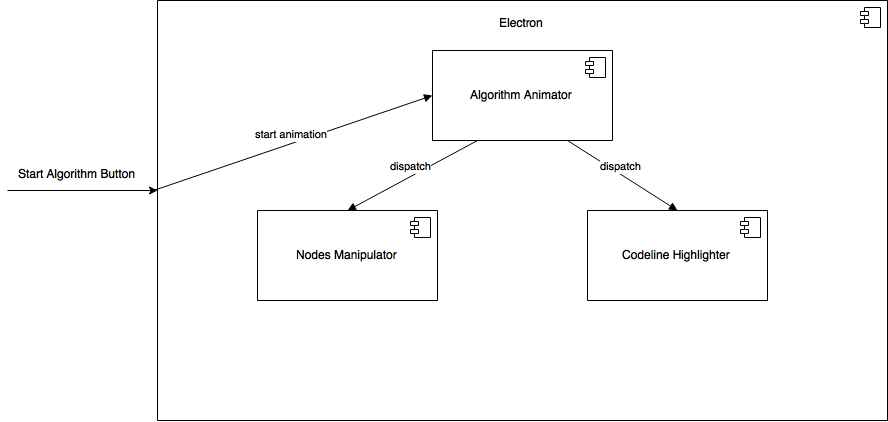
\includegraphics[scale=0.45]{UML_component_diagram}
    \caption{UML component diagram.}
    \label{fig:uml-component-diagram}
\end{figure}

It can be noticed that our approach was rather simplistic - after the user hits the start algorithm button, the main
component is the Electron window. This is, in fact, the native window generated by the framework which contains the application. As we will see in the subsequent sections, Electron makes use of web tools (i.e. CSS, HTML5 and JavaScript) to animate the objects on the
canvas. The algorithm animation will be made out of 2 components: the node manipulator which will colour, move,
hide and change the vertices of the graph or tree, while the codeline highlighter will handle the animation of the
algorithm's codelines. They will execute concomitantly and generate output immediately in the window.

Therefore, our architectural style of choice is component-based: every algorithm is a component itself and they all
interact with the Electron core functionality such as windowing, copy-paste-cut, system calls etc. It emphasizes on
reusability through loosely coupled independent components, thus adding simplicity to the project and making it
scalable and maintainable.

\section{Application Type}

This was a very important question right from the beginning. Having the experience from past years students who
implemented algorithm animators, creating a Java application that could be packaged into a JAR seemed attractive. Java is the
language used the most for university coursework, thus there was comfort in choosing this approach.

Also, there are many projects available that were of interest. The one we studied closely before deciding on whether to
choose Java or not as the primary language behind our animator was ANIMAL~\cite{animal-algo-animation}, one of the most popular tools on the
web. Even though the paper published by Rößling et al.\ is almost 20 years old, the animator is still actively under
development, the latest release dating back to 5th of September 2016.

\begin{figure}[!ht]
    \centering
    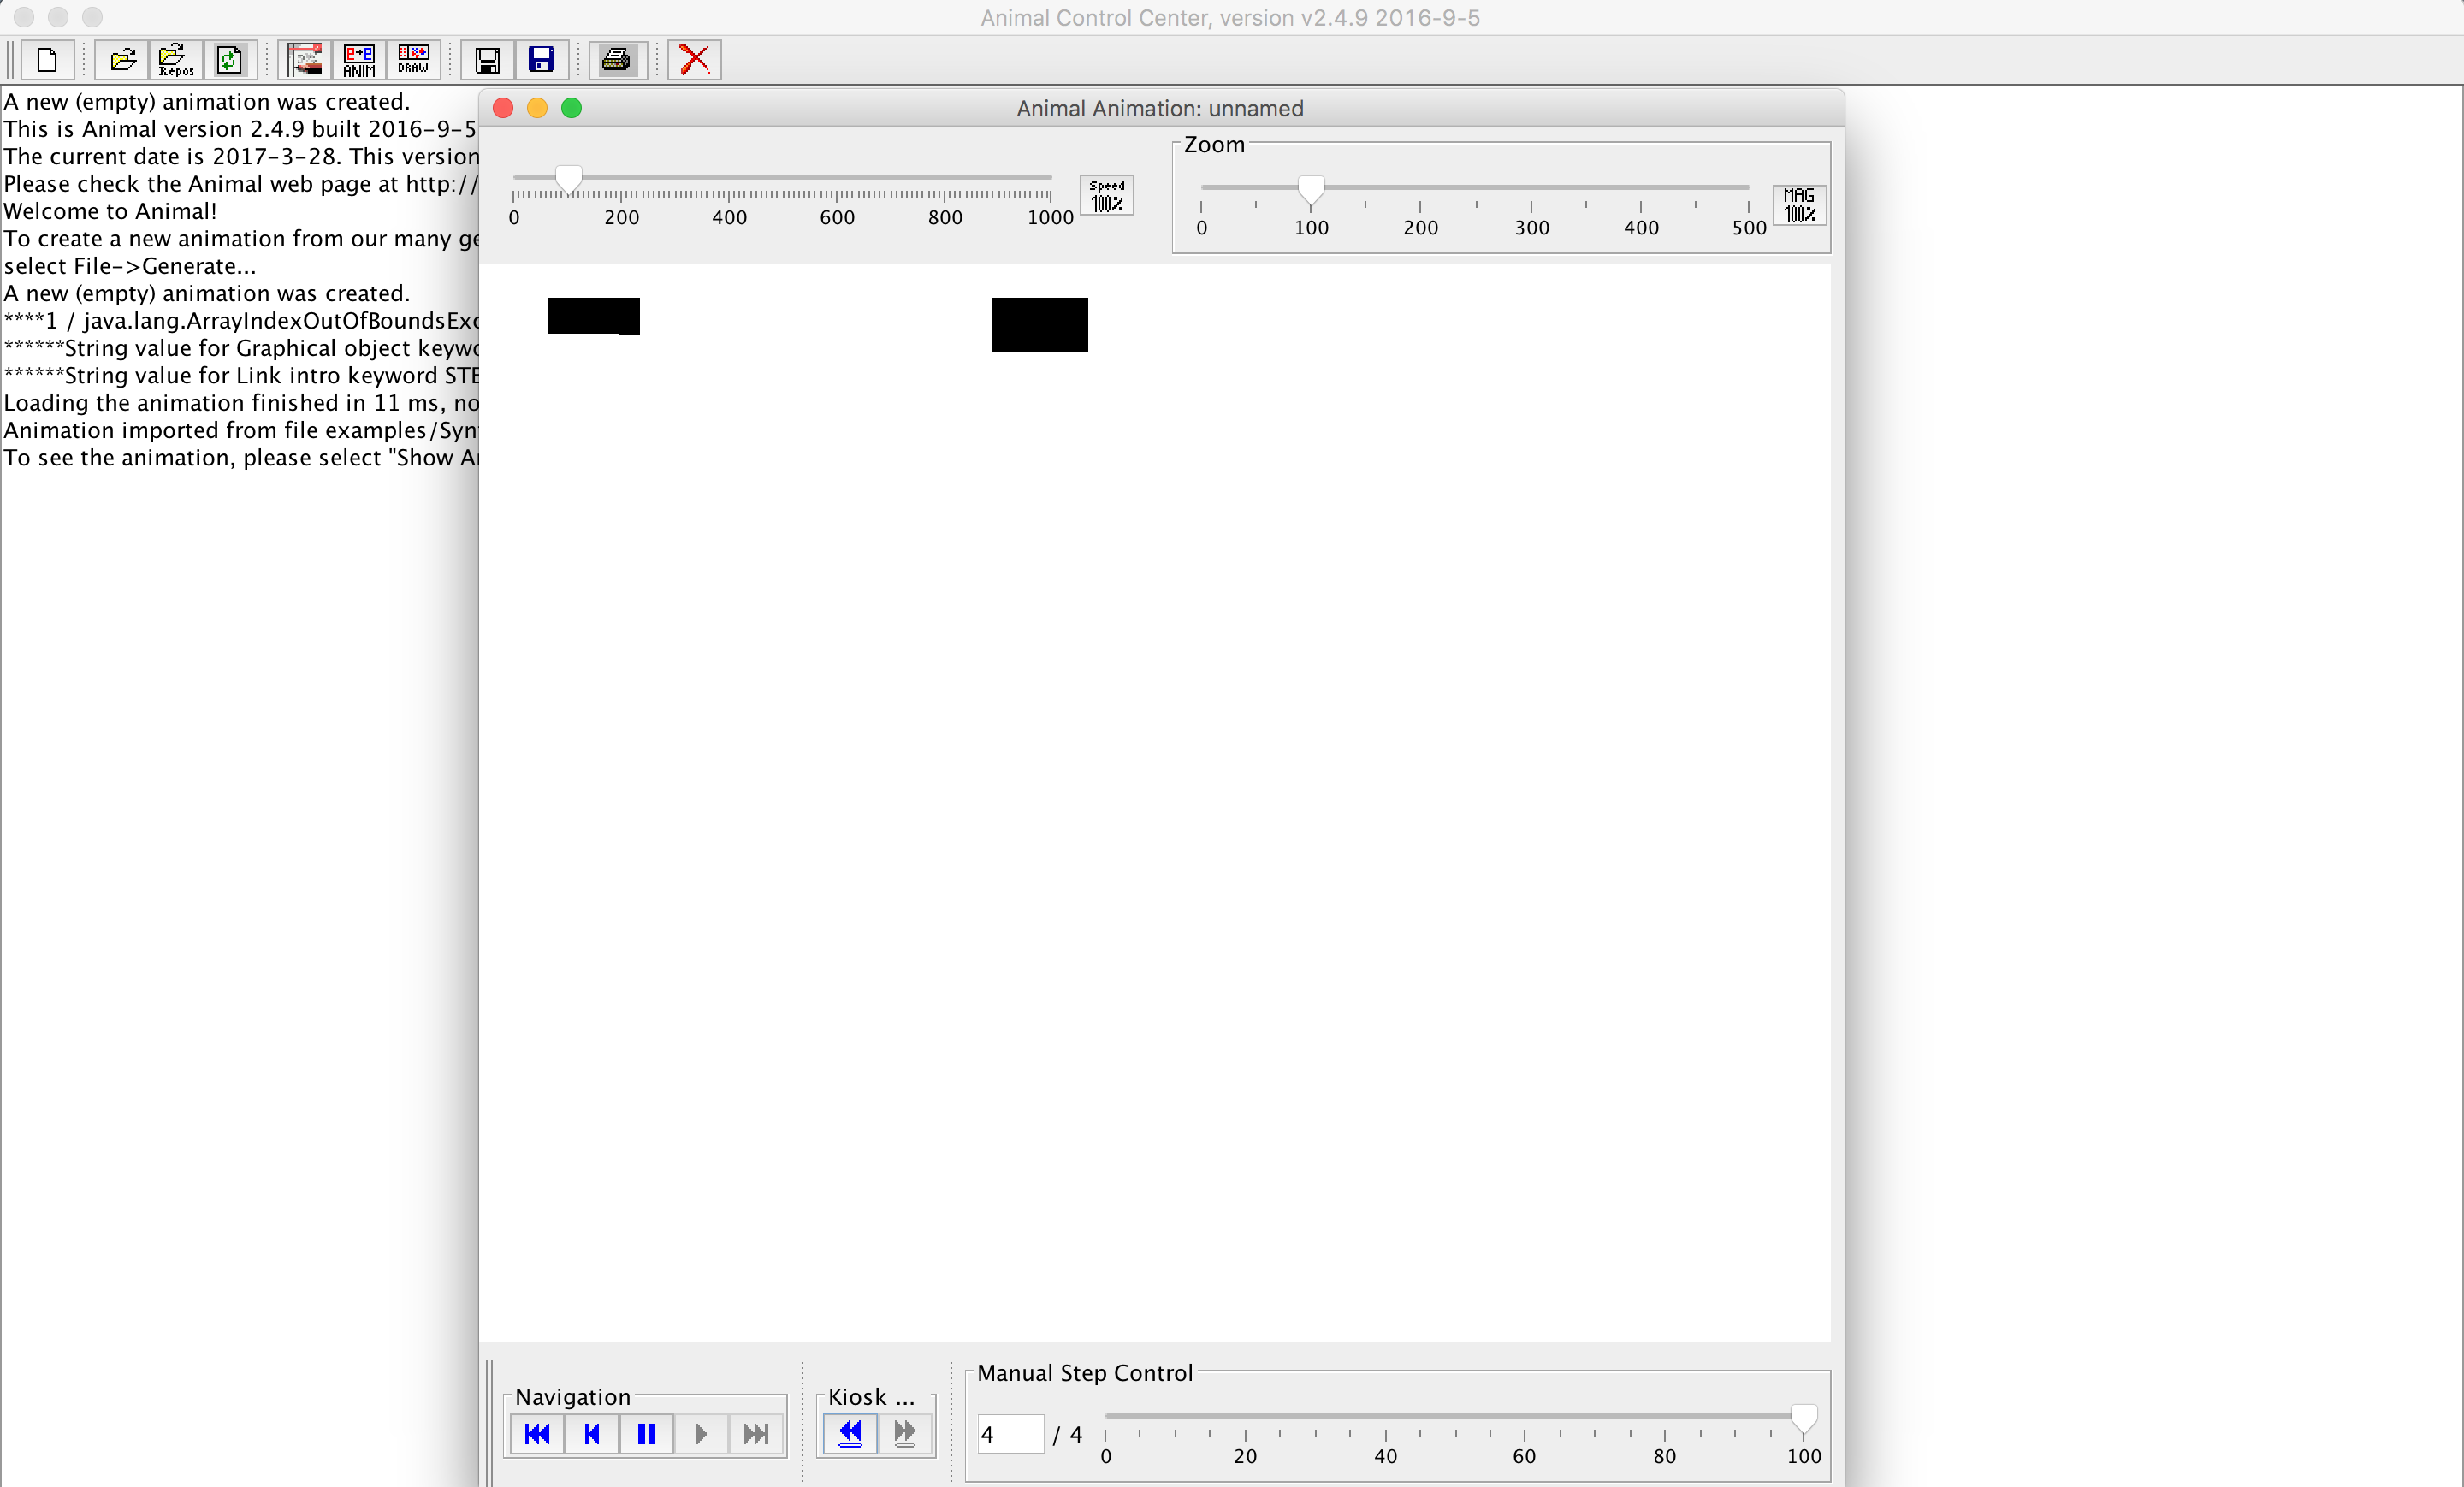
\includegraphics[scale=0.25]{animal-algo-animator}
    \caption{Screenshot taken while using the Animal algorithm animator.}
    \label{fig:animal-algo-animator}
\end{figure}

The screenshot in Figure~\ref{fig:animal-algo-animator} shows how many options are available to the user and how powerful the application is, providing
features such as the possibility to create
your own algorithm, animate it the way you want to, set any colour for blocks and even draw manually.

On the other hand, the other option that we considered was making an animator based on web tools. The first and obvious
approach was to create a website using the very large number of libraries for drawing on the canvas and manipulating
the Document Object Model (DOM) in general. Firstly, we began by investigating how popular JavaScript was among developers and if this was
feasible after all. Figure~\ref{fig:stack-overflow-languages} presents a recent survey from StackOverflow, one of the most comprehensive and useful resource repository for developers around
the globe~\cite{stackoverflow-survey}.

\begin{figure}[!ht]
    \centering
    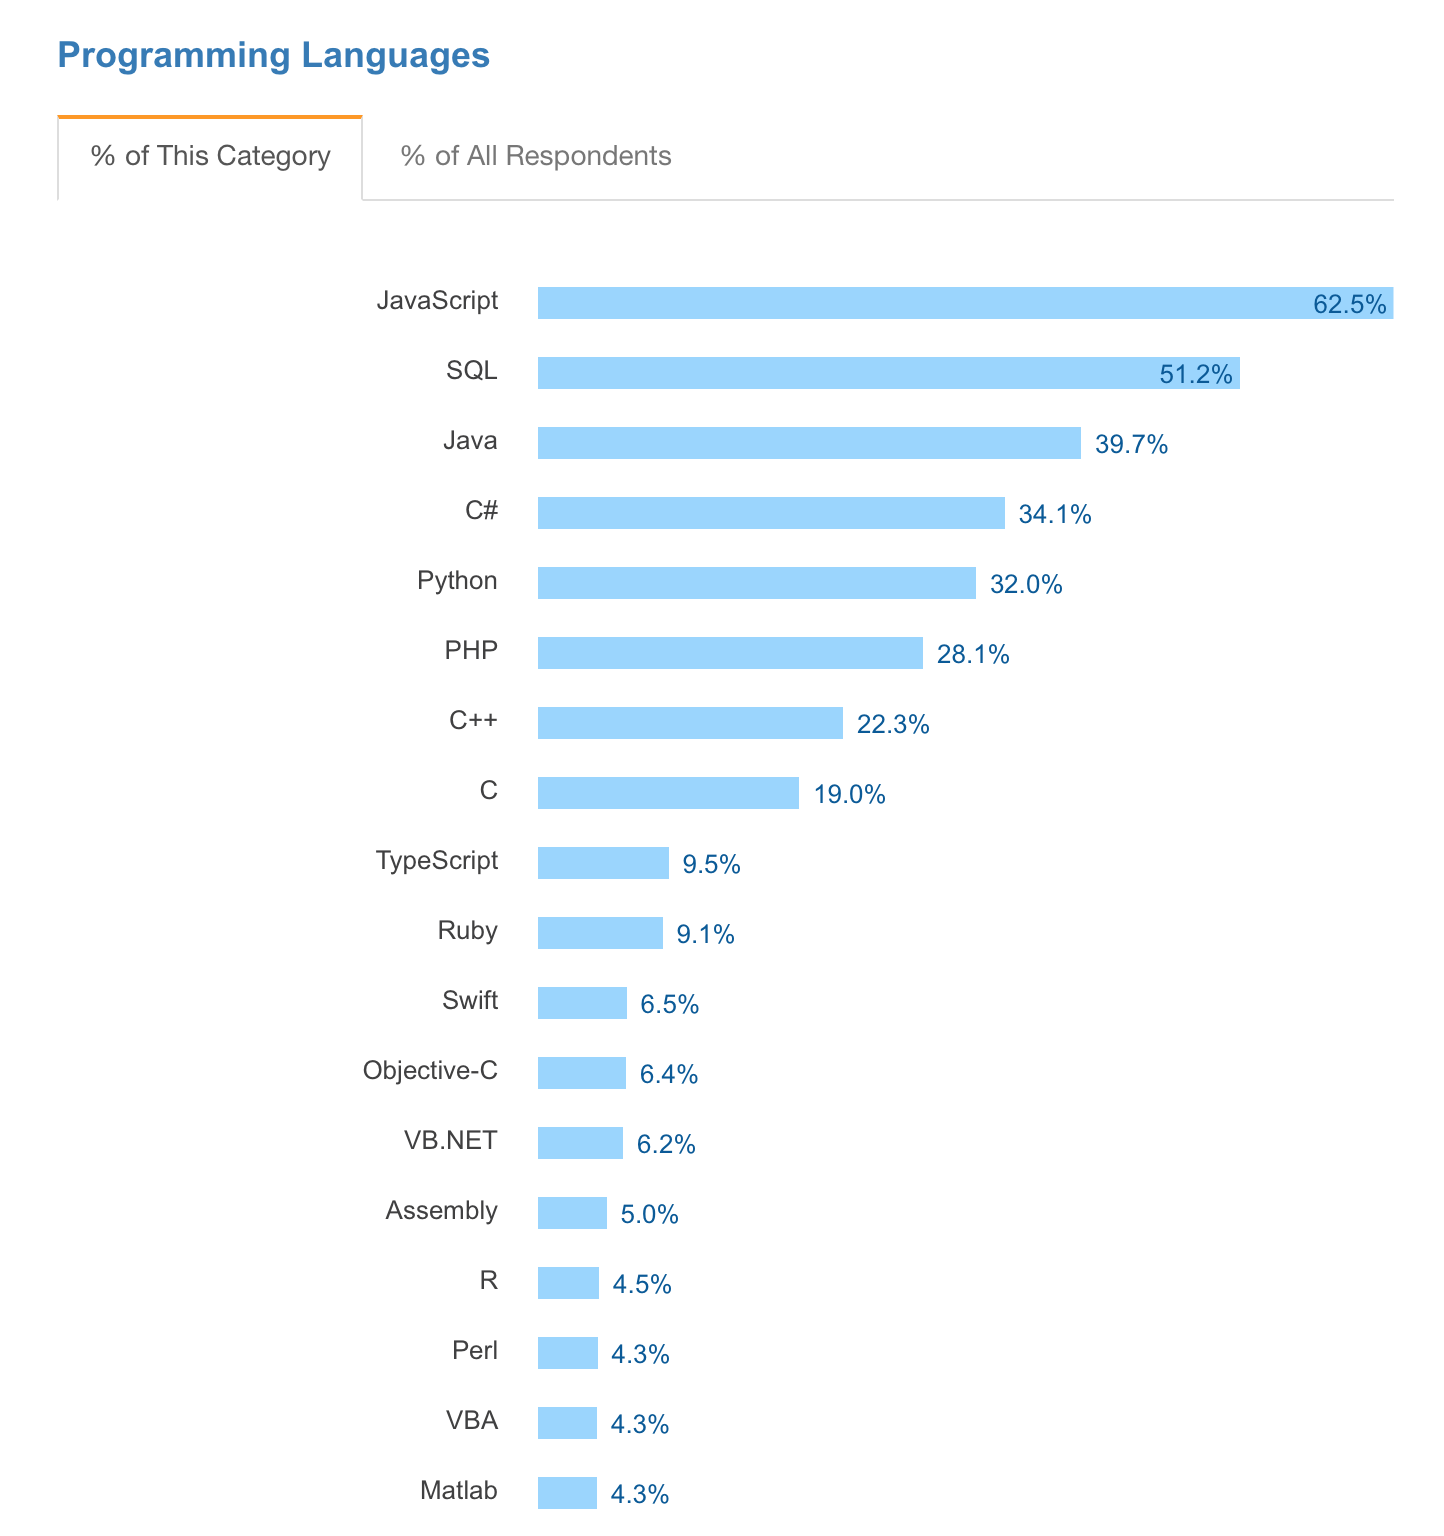
\includegraphics[scale=0.5]{stack-overflow-languages}
    \caption{Most popular 18 programming languages in 2017.}
    \label{fig:stack-overflow-languages}
\end{figure}

As it can be seen, JavaScript is almost twice as popular as its competitor Java. Also, when talking about concrete JavaScript libraries, there is a considerable amount published as open source. Other advantages for this approach were:

\begin{itemize}
    \item great reach to users as almost everyone has at least a browser installed on their machine;
    \item modern, state-of-the-art UI libraries that would make the experience pleasant for users.
\end{itemize}

Weighing both options, we eventually decided to proceed with the web approach because our main goal was to make users, especially students who want to learn new algorithms, enjoy using our animator. Web tools, as discussed previously, provided us with a variety of User Interface components that made our goal possible.

\section{Prototyping}

Following Agile methodologies implied that we would involve the potential customers during the whole process in order
to get continuous feedback. Therefore, we developed low fidelity prototypes in the early iterations (i.e.
paper-based) and eventually high fidelity ones (mainly using Omnigraffle~\cite{omnigraffle}).

Figure~\ref{fig:paper_prototype} presents one of the early paper drawings that could give our users an idea of how the animator might look
like.

\begin{figure}[!ht]
    \centering
    \includegraphics[scale=0.06]{paper_prototype}
    \caption{Low fidelity prototype drawn during one of the early sprints.}
    \label{fig:paper_prototype}
\end{figure}

As you can notice, the prototype is very basic but we wanted to give the end users a rough outline of how the application will
look like. Mostly, it resembles what Palgo looks like in the latest version, especially the layout of the two animation
panes as well as the position of the logo.

However, as iterations passed, we started building high fidelity prototypes and we used more mature tools to wireframe
such as the above-mentioned Omnigraffle. Figure~\ref{fig:high_fidelity_prototype} shows one of our prototypes from
late January.

\begin{figure}[!ht]
    \centering
    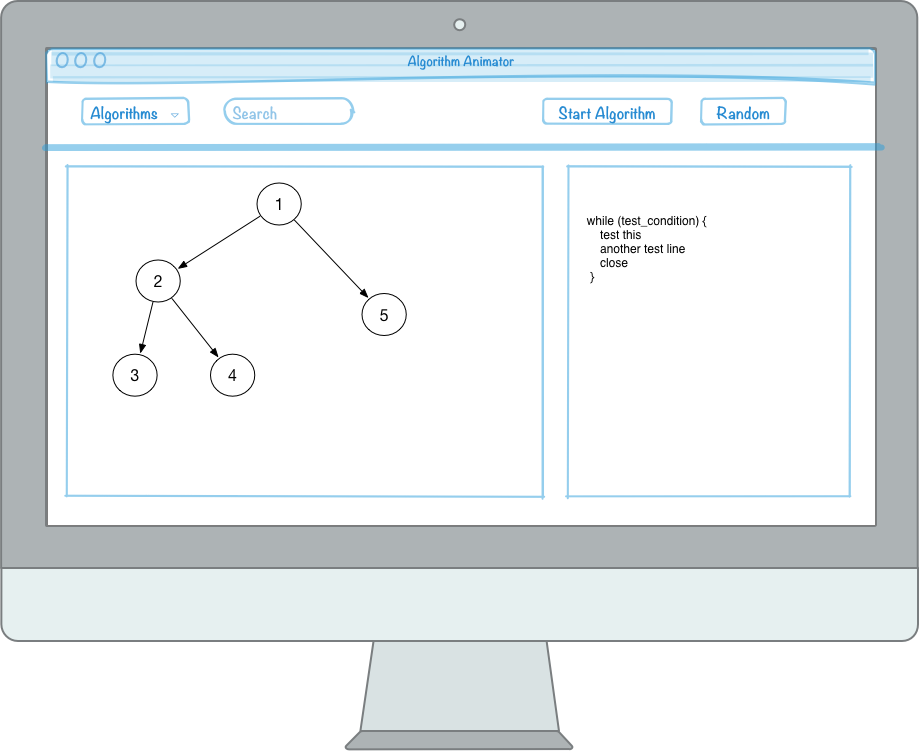
\includegraphics[scale=0.3]{high_fidelity_prototype}
    \caption{High fidelity wireframe built with Omnigraffle.}
    \label{fig:high_fidelity_prototype}
\end{figure}

We soon afterwards started demonstrating the application itsself without the need of wireframing, as the animator began to be
mature enough and provide a minimum of functionalities that could give the testers a better idea of how everything
works compared to a simple image that we showed to them.

As it can be seen from the first paper prototype up to the higher fidelity ones the design we came up with was very
similar to the one the application has nowadays. However, the buttons were moved from the right hand side to the left because
of the users' feedback - they requested that they should be below the bar with the logo so that the UI would be cleaner with the elements more easily distinguished. Also they requested to remove the search bar as they found
it useless except if the number of algorithms grew considerably and a dropdown would have ruined best UI/UX practices.

\section{Electron}

Thus, we ended up with using a web approach. There are many options available, ranging from university-specific algorithm animators to more general ones such as the previously mentioned VisuAlgo~\cite{visualgo}.

However, one very important aspect that we were concerned about was the core underlying principle of the internet, which is that it requires a permanent internet connection. What if our users would not have access to internet a couple of days before an algorithmics exam? What if our potential user would want to play around with algorithms at his/her own pace without needing to have a wired or wireless connection?

Also, another thing we had to think about was UI and UX engineering. Having maybe too many resources available, we could have ended up with choosing one that would not fit a part of our users. How can we make sure that the framework we would decide on will make all users feel familiar?

Therefore, the best approach would be to have an animator that is implemented using web tools but can function as a standalone desktop application. Thus, by being native, it would make all users feel familiar in any their operating system of choice. At this point, we had to research different alternatives to create cross-platform native applications with web tools. The one that was most popular and had the largest library of resources was Electron, which we chose in the end.

Electron is a framework built by engineers at GitHub and then released as an open source project on their platform. It is in fact a Chromium backend that serves webpages inside windows which act as native regardless of the platform of choice. Therefore, the developer can use any web tools available to develop his/her applications benefiting at the same time from features such as system calls.

Because it is uses Chromium under the hood, we are automatically taking advantage of the V8 engine~\cite{v8-chrome} which powers the Google Chrome browser. Efficiency was primordial to us and such we wanted to check if such a candidate would produce exptected output in a reasonable time, so we checked benchmarks available for various JavaScript engines.

\begin{figure}[!ht]
    \centering
    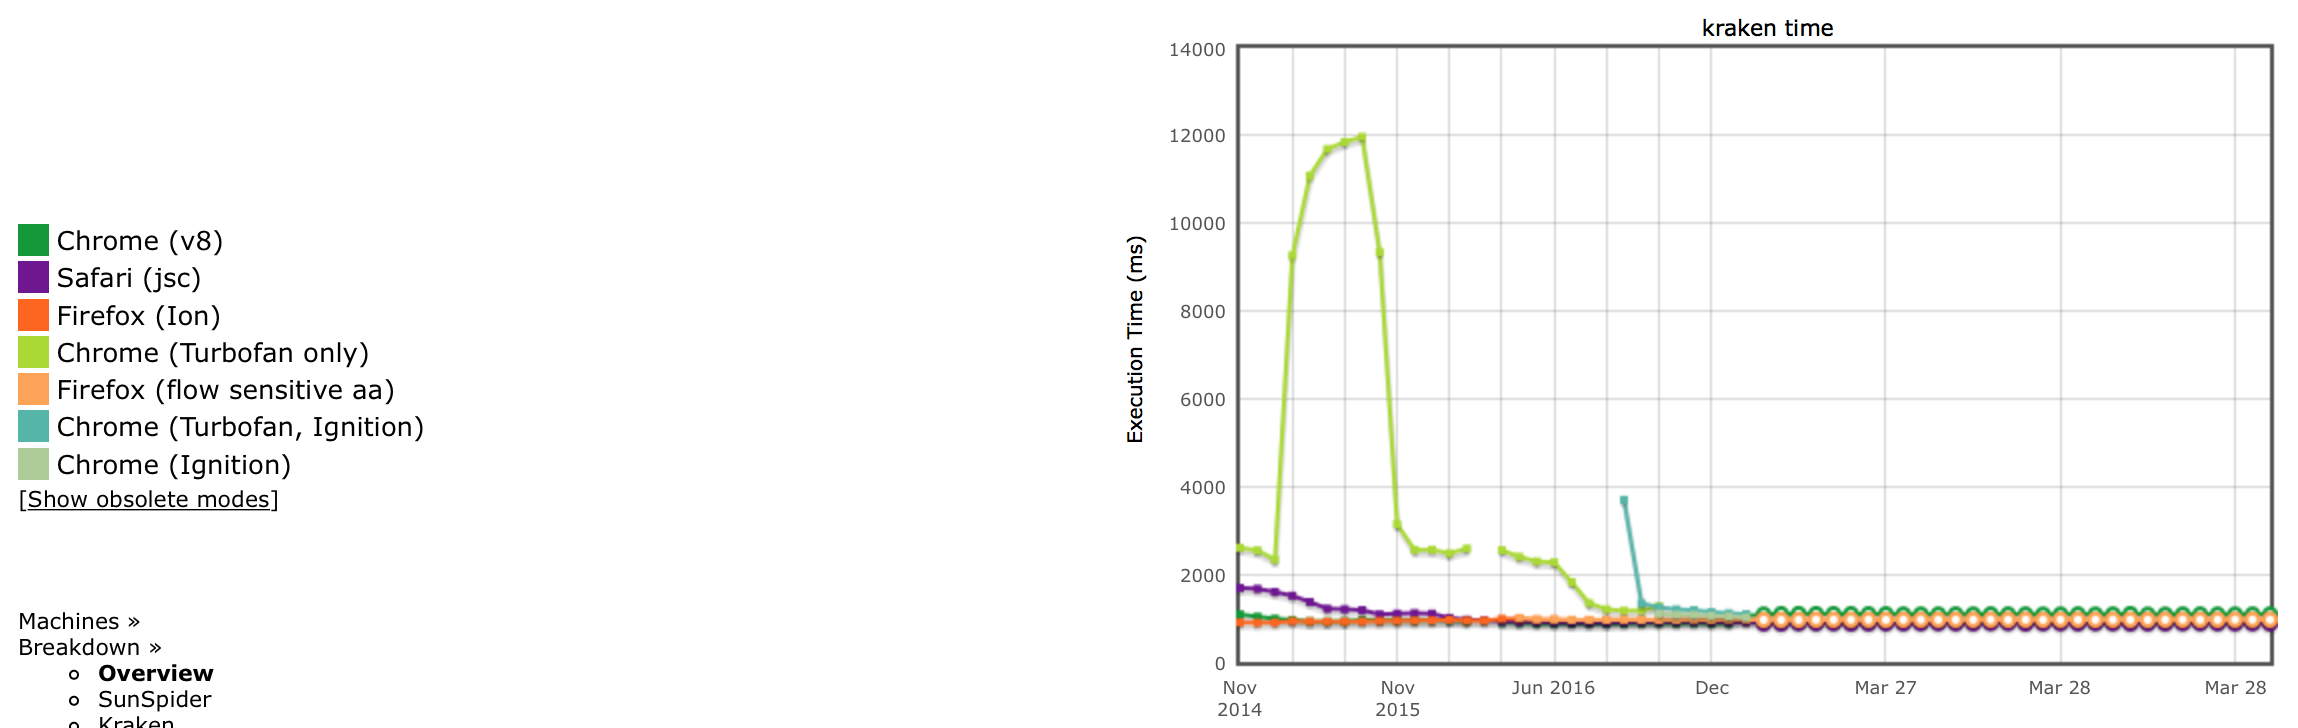
\includegraphics[scale=0.35]{v8-benchmark}
    \caption{Benchmarks for various JavaScript libraries as of 28/03/2017.}
    \label{fig:v8-benchmark}
\end{figure}

Figure~\ref{fig:v8-benchmark} shows benchmarks for various JavaScript engines including jsc, Ion and V8. As we can see in the
figure, V8 ranks extremely highly, being at the lowest points of execution times starting almost from its inception.

The other very important aspect was to see if Electron had enough resources, tutorials or demo applications to allow the
the development workflow to be smooth.
We ran a query on Google Trends among other platforms to check how popular it was.
Figure~\ref{fig:google-trends-electron} presents the results.

\begin{figure}[!ht]
    \centering
    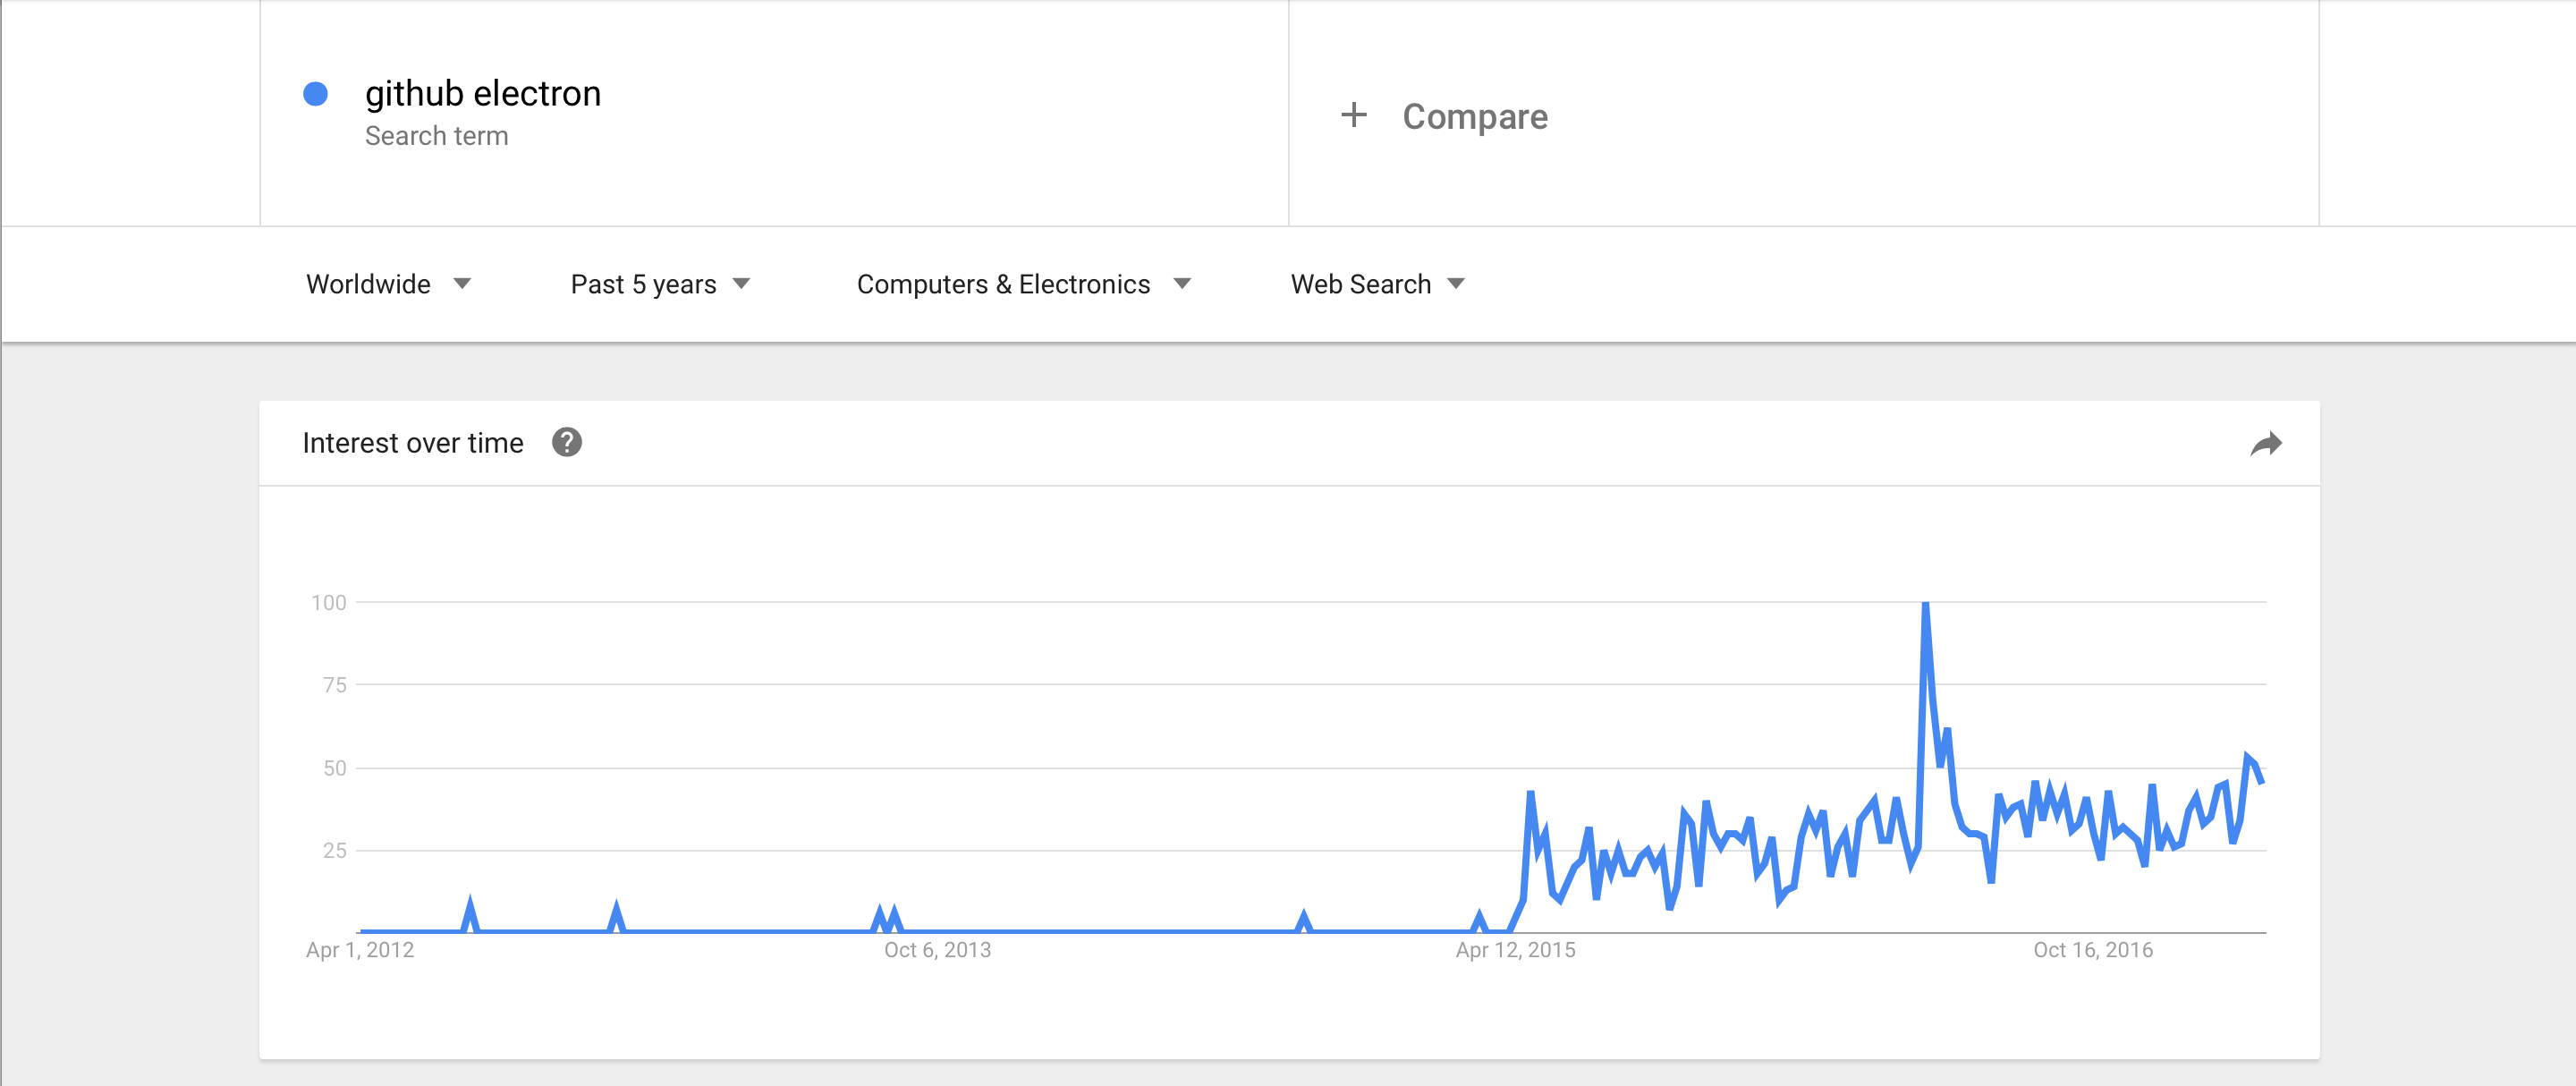
\includegraphics[scale=0.35]{google-trends-electron}
    \caption{Electron trending on Google in the past 5 years.}
    \label{fig:google-trends-electron}
\end{figure}

We can clearly observe that apart from the big spike when the framework became the underlying engine behind many
important desktop apps such as Slack towards the end of 2015, Electron has had an constant ascension throughout the
years. Also, researching the internet for resources, we found many tutorials and demo applications from which we could draw inspiration.

Summing up, Electron was a natural choice after careful thinking about advantages and caveats and it proved to be a very productive framework that allowed an easy and simple workflow for the rest of the software development lifecycle.

\section{Drawing}

The component that had the same importance as Electron was the engine behind manipulating the vertices and edges of trees and graphs as trees and graphs were the focus of the algorithms to animate. Because of the large variety of JavaScript libraries available for playing with the canvas, we had a couple of choices to select from. This was a very lengthy process because many provided some features while others gave us other unique ones. 

Table~\ref{drawing-libraries} presents the libraries together with their pros and cons.

\begin{table}[!ht]
\centering
\resizebox{\textwidth}{!}{%
\begin{tabular}{|l|c|c|c|c|c|c|}
    \hline
    & \multicolumn{1}{l|}{Vertex Manipulation} & \multicolumn{1}{l|}{Edges Manipulation} & \multicolumn{1}{l|}{Tree API} & \multicolumn{1}{l|}{Graph API} & \multicolumn{1}{l|}{Actively Maintained} & \multicolumn{1}{l|}{Easy Pick-Up} \\ \hline
    Treant       & \Checkmark                                       & \Checkmark                                       & \Checkmark                             & x                              & x                                        & \Checkmark                                 \\ \hline
    Vis JS       & \Checkmark                                       & \Checkmark                                       & \Checkmark                             & \Checkmark                              & \Checkmark                         &            \Checkmark                                 \\ \hline
    Sigma Js     & \Checkmark                                       & \Checkmark                                       & \Checkmark                             & \Checkmark                              & \Checkmark                                        & x                                 \\ \hline
    HTML5 Canvas & x                                       & x                                       & x                            & x                              & \Checkmark                                        & x                                 \\ \hline
    D3           & \Checkmark                                       & \Checkmark                                       & x                             & x                              & \Checkmark                                        & x                                 \\ \hline
\end{tabular}%
}
\caption{Table showing features provided by the main drawing libraries for trees/graphs.}
\label{drawing-libraries}
\end{table}

As shown in the figure, the main candidates we have chosen for the drawing libraries are VisJS, Treant, D3, HTML5 Canvas and SigmaJS. Let us start with Treant. This was a very compelling option because it had a very robust and easy to use Tree API: vertices
and edges could be easily manipulated, as well as the layout was very flexible to suit the developer needs. However, as
it can be seen in the table above, we did not have an out-of-the-box API for graphs. Therefore, this option became unfeasible.

HTML5 Canvas is a component defined by W3 Consortium themselves and thus it's actively under development and heavily
standardized. However, apart from continuous maintenance and new regular features, it is hard to pick up and it does
not provide APIs specifically designed for graphs or trees which meant we needed to put too much effort in learning a
new platform rather than focusing on actual implementation of the animations.

D3 and SigmaJS are both very mature platforms that have a very large number of features for animating and drawing on
the canvas. They were both viable candidates up until the end. However, the reason why we eventually chose VisJS
is because it was the easiest to pick up and had out-of-the-box APIs for both graphs and trees. Thus, choosing VisJS, we saw a rapid development workflow and an emphasis on simplicity due to the fact that the tools
we were using were not standing in our way, but rather helped us to quickly implement the user stories.

\section{Animation}

After drawing, the next major issue we had to discuss was the actual animation part. We have researched many tools
available and we ended up with basic set timeouts. Listing~\ref{js-animation-snippet} depicts a code snippet used for
animating the codelines followed by a reset of the whole graph to its initial state.

\begin{lstlisting}[language={Java}, label={js-animation-snippet}, caption={JavaScript snippet for creating an
animation.}]
setTimeout(
  function() {
    unHighlightAllCodeLines();
    for (var k = 0; k < nodesArrayLength; k++) {
      unHighlightTableCell(nodes[k].label);
    }
    resetWholeNetwork(network, container, options);
  },
  2000 + 3000 * nodesArrayLength + 13000 * nodesArrayLength - 1
);
\end{lstlisting}

Even though the implementation details will be covered in the following chapter, we shall discuss here the importance
and the reason why we decided to use this approach instead of others. Some libraries were already built to facilitate developers an easy path to animation, so why use plain JavaScript for
accomplishing this? We have reviewed and discussed advantages and disadvantages for the following JS libraries for animation:

\begin{itemize}
    \item Velocity JS;
    \item DOM JS Animation;
    \item JQuery Animation.
\end{itemize}

Unfortunately, we had to give up all these options because the main issue with using any of them was that they are
manipulating elements which are part of the DOM (Document Object Model), while in our project the elements (i.e. nodes
in the tree/graph) are part of
the canvas, thus they are not individual components of the DOM. Therefore only the canvas could be animated as a whole without being able to manipulate the individual elements inside.

Having discussed all these caveats, we were left with no other choice than devise algorithms to animate our nodes and
codelines using plain setTimeout calls throughout the project. Even though it was a compromise and it slowed
drastically the workflow in the beginning, once we passed the steep learning curve, we were able to animate all the
elements in short periods of time.

\section{Material Design}

We had a couple of main possiblities to choose from when designing the application's User Interface:

\begin{itemize}
    \item Material Design by Google;
    \item Bootstrap by Twitter;
    \item Pure CSS.
\end{itemize}

There were others as well, such as Base~\cite{base-ui} or Simple Grid~\cite{simple-grid-ui}, but these were not specifically suitable for
our purposes. Therefore, we shall analyze different benefits given by the 3 above mentioned platforms and why we
eventually ended up with Material Design by Google.

In Figures~\ref{fig:bootstrap-navbar},~\ref{fig:material-design-navbar} and~\ref{fig:purecss-navbar} we shall present
different design approaches for one of the most used and noticeable components to a user when they interact with an
application, which is the navigation bar.

\begin{figure}[!ht]
    \centering
    
\includegraphics[scale=0.35]{bootstrap-navbar}
    \caption{Bootstrap default navigation bar.}
    \label{fig:bootstrap-navbar}
\end{figure}

\begin{figure}[!ht]
    \centering
    
\includegraphics[scale=0.35]{material-design-navbar}
    \caption{Material Design navigation bar.}
    \label{fig:material-design-navbar}
\end{figure}

\begin{figure}[!ht]
    \centering
    
\includegraphics[scale=0.35]{purecss-navbar}
    \caption{Pure CSS default navigation bar.}
    \label{fig:purecss-navbar}
\end{figure}

We can clearly notice a more colourful, natural and playful approach in the Material Design navigation bar. We have
presented all 3 options to the level 4 students and they were all in favor of the Material Design UI for all components
(more details on the results of these evaluations in Chapter~\ref{testing}, section Prototype Evaluation).

Even though the Material Design components were invented by Google (which are also available on GitHub), we have opted for the ones open sourced by Federico
Zivolo~\cite{material-design} because they are much more popular and there are more resources with which one can get
accustomed to faster. 

We have decided to use this approach for several reasons:

\begin{itemize}
    \item Material Design has gained much more traction than the other frameworks since its inception;
    \item even though Pure CSS does not require any JavaScript dependencies (hence the name), it is very raw and it
	requires a lot of tweaking before going into production;
    \item Bootstrap is the foundation of virtually every framework available but it is exactly that, a foundation, thus
	it does not give the developer advanced features out-of-the-box.
\end{itemize}

\section{Compromises}

One of the compromises mentioned previously as well was that we had to use setTimeouts to animate our objects instead
of mature, easy-to-grasp libraries. What the setTimeout function does is it sets the execution of the callback function
provided at a specific time in the future. Because we had only a canvas and we could not manipulate vertices as regular DOM
objects, all the vertex colouring and label changing was done using a chain of setTimeouts that, at the beginning of the
algorithm (i.e. when the user presses the ``Start Algorithm" button), they would have their exact time calculated as to
when they got executed. One example is: colour this vertex at millisecond 2600, change its left
children's label to 2 at millisecond 3500 and finally highlight the codeline ``set label to 2" at the same time, 3500.
This was extremely hard to understand and master and the first iterations were quite slow. However, as time passed and
I gained more experience with this technique, development became much easier.

Another compromise that we needed to take was the lack of play/pause, previous and next buttons for the animator.
Figure~\ref{fig:play-pause-previous-next} presents a screenshot taken while using VisuAlgo.

\begin{figure}[!ht]
    \centering
    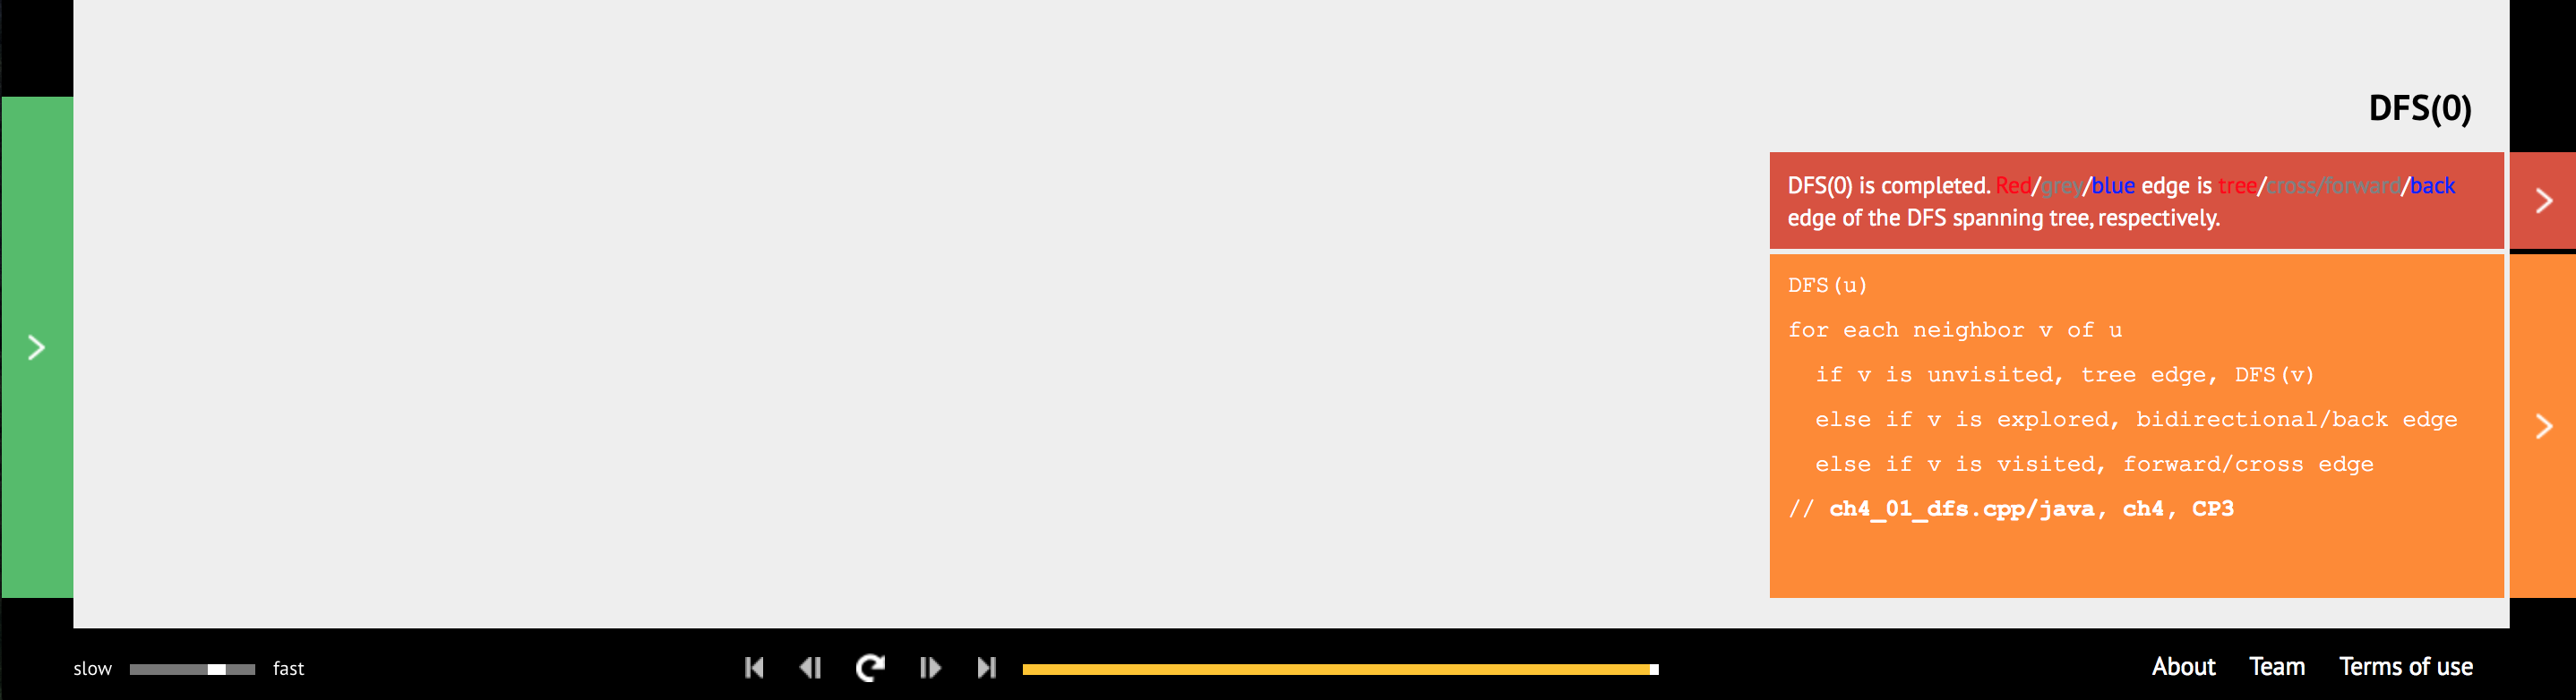
\includegraphics[scale=0.35]{play-pause-previous-next}
    \caption{VisuAlgo play/pause/previous/next buttons for the animator.}
    \label{fig:play-pause-previous-next}
\end{figure}

This is a functionality desired by most of our users as well as Dr. Norman. However, due to the previous compromise we
have stated (i.e. using setTimeouts for animating the algorithms), it was virtually impossible to mimmick these
buttons.

%==============================================================================

\chapter{Implementation}
\label{implementation}

In this chapter we will discuss how the project was actually implemented, how we overcame the
JavaScript shortcoming of not having multi-threading support, as well as how other various functionalities were put
into place. We will conclude by talking about the main issues faced and what lessons were learned. 

\section{Algorithm Selection}

The algorithm selection was solely done during the supervisor meetings. We have come up with the following list of algorithms:

\begin{itemize}
    \item Huffman tree construction;
    \item Heap insertion and deletion;
    \item Depth-First Search in a graph;
    \item Breadth-First Search in a graph;
    \item Dijkstra's Shortest Path;
    \item Prim-Jarnik's Minimum Spanning Tree;
    \item Dijkstra's Refinement of Prim-Jarnik's Minimum Spanning Tree.
\end{itemize}

These candidates were chosen because they are all among the most common and used algorithms and they are also very
popular among university computer science courses. We have taken the codelines which would be animated from Dr.
Norman's slides from the Algorithmics I class at University of Glasgow. Moreover, we also double checked them for correctness. They were translated from either pseudocode or Java to JavaScript which implied rather simple transformations as
the languages do not have such divergent syntaxes. 

\section{Project Structure}

We have split our application into 3 main components, as in traditional website development: stylesheets, JavaScripts
and HTML5 pages. They were all coordinated by npm which is the node package manager~\cite{npm}. Essentially,
npm is the equivalent of Maven or Gradle for Java projects and  is both a dependency manager and a build automation
tool. Therefore, in npm we defined the name of the project and all sorts of metadata as well as the dependencies needed
for building the app. As soon as all these were set, we started working on the three main categories of files mentioned
above. Figure~\ref{fig:project-structure} presents the simple structure we opted for.

\begin{figure}[!ht]
    \centering
    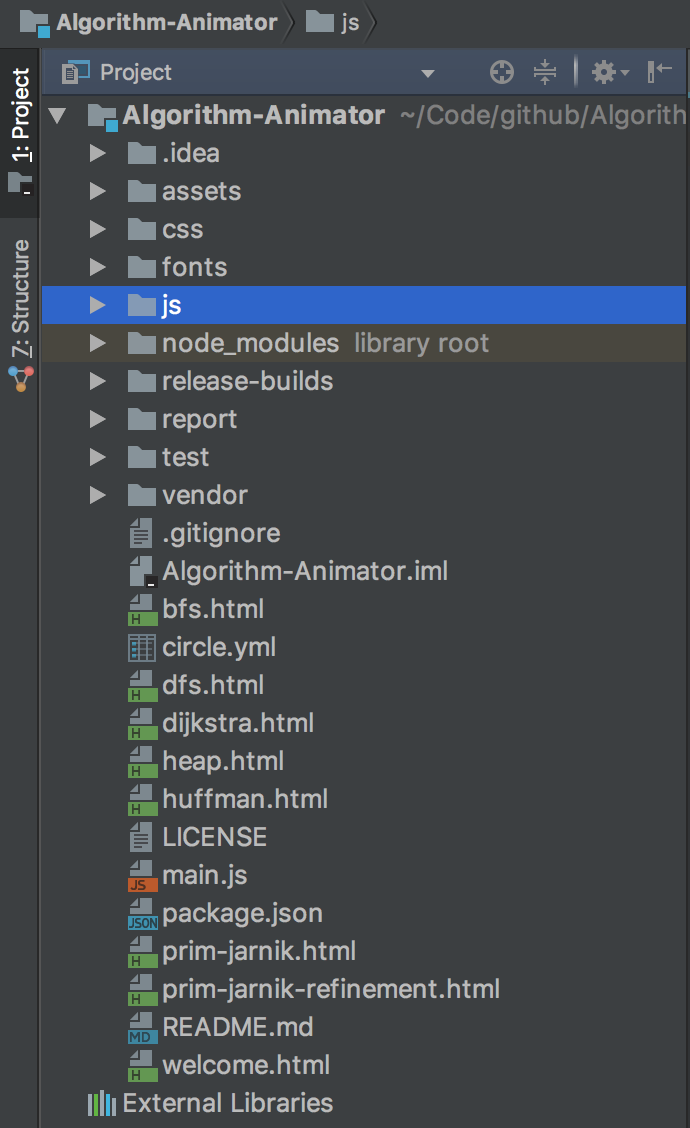
\includegraphics[scale=0.4]{project-structure}
    \caption{Project Structure as shown in Intellij IDEA.}
    \label{fig:project-structure}
\end{figure}

Architecturally speaking, because we have opted for a Component Based approach, everything is built so that it can be
reused. Therefore, the nodes animators for all algorithms, as well as the codeline animators, are generic and only
adapted to the specific algorithm. 

Also, we have also added in assets, vendor and fonts components. These are just static files that will be used to render fonts,
add images to the HTML pages as well as provide some extra JS modules to the specific algorithm animators. 

Last but not least, the package.json file is automated so that we can add the releases as easy as possible to the
release-builds folder which will contain all executables for the 3 main operating system families: macOS, Windows and
Linux.

\section{Animation Pipeline}

After the user presses the Start Algorithm button there is a pipeline of processes that run ``behind the
scenes". This pipeline is display in the UML use case diagram shown in
Figure~\ref{fig:animation_uml_use_case_diagram}.

\pagebreak

\begin{figure}[!ht]
    \centering
    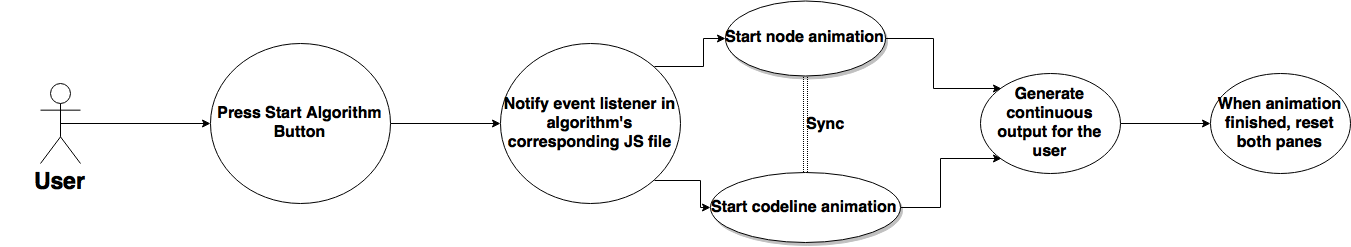
\includegraphics[scale=0.3]{animation_uml_use_case_diagram}
    \caption{UML Use Case Diagram showing application flow of events.}
    \label{fig:animation_uml_use_case_diagram}
\end{figure}

As it can be seen, everything starts when the user presses the start algorithm button present on every page. From
there, the event listener is set to check if the user clicks the button (in the corresponding JavaScript
file) and starts the 2 animation components. The two components are always in sync being set to execute at the same time using the setTimeout delay functionality (e.g.\ both do iteration $x$ after 1000 milliseconds multiplied by $x$), thus giving the user
synchronous output from the nodes pane and codelines pane. When they have executed their last iteration, they
both stop and the whole canvas is reset to its original state. This is done again with a setTimeout call with the delay
set as unit of time (usually 1000 milliseconds) times the total number of steps to complete the algorithm. The number
of steps is either computed automatically (e.g.\ in Huffman tree construction we can directly calculate the total number
of steps needed to complete the animation) or through running the algorithm in the background and returning the value.
As we discussed previously, the V8 engine is extremely fast thus the execution of any of our algorithms is in terms of
milliseconds, the delay being indistinguishable for the human eye. 

One concern might arise and that is: even though executing the algorithm an unnecessary extra time would not make the
user notice any difference, why do it after all? Let's take the following example from the heap insertion algorithm
(Listing~\ref{insert_heap}).

\begin{lstlisting}[language={Java}, label={insert_heap},caption={Pseudocode for inserting a node in a heap.}]
insert item in new leaf node; 
while (new_value not in root && new_value > parent_value) {
    swap new_value with parent_value;
}
\end{lstlisting}

As you can see here, we have a while loop, therefore we do not have an already known number of steps until the
condition fails and we exit the loop (as we would generally have in a for loop). Listing~\ref{javascript-insert-heap}
shows a part of the actual implementation for
animating an insertion in a heap.

\begin{lstlisting}[language={Java}, label={javascript-insert-heap}, caption={Actual implementation for animating the
insertion of a heap node.}]
const steps = getInsertSteps(node);
for (let index = 0; index < steps; index++) {
  (function(i) {
    highlightHeapCodeLine("insert", 2);
    arrayOfSetTimeouts.push(setTimeout(
      function() {
	if (prev) {
	  prev.color = "#009688";
	}
	prev = cursor;
	let tempLabel = cursor.label;
	cursor.label = cursor.parent.label;
	cursor.parent.label = tempLabel;
	cursor.color = "red";
	cursor.parent.color = "red";
	cursor = cursor.parent;
	network = rebuildHeap(nodes, edges);
      },
      1000 + i * 1000
    ));
  })(index);
}
\end{lstlisting}

We can see that we are first getting the number of steps (the constant variable steps) and then executing a for loop with the test condition being
that index is smaller than steps. Then, we are passing index as a parameter to the self-invoking function inside the
for loop. On line 19 you can observe how we are delaying that function using the parameter $i$ which in turn is index
from the outer loop. Imagine that we had a while loop instead of this and we started the algorithm animation. The first
step was that as the interpreter would start fetching, reading and executing the source code, it would go into an
infinite loop as soon as it hit the while (test-condition) line. This would happen because it would not execute the
inner code (i.e. swapping the new value with the parent value; this is because when a setTimeout is read by the
interpreter, what is
inside is never executed until that specific delay set by the developer), thus progressing towards meeting the condition and
breaking the loop. However, in
a for loop $i$ is incremented until it breaks the test condition and the loop is exited.

On the other hand, we have implemented algorithms that do not require an extra execution, such as Dijkstra's
Shortest Path. There we would just call the for loop directly and animate the 2 panes synchronously.

\section{JavaScript Multi-Threading}

This was the most important issue faced throughout the whole software process. Because I did not have previous
experience with web applications that might require multi-threading support, I did not know if JavaScript provides this
or not. In Listing~\ref{dijkstra-animation} we provide a code snippet first to better describe the problem and discuss
on it afterwards.

\begin{lstlisting}[language={Java}, label={dijkstra-animation},caption={Animation function used in Dijkstra's SP
algorithm.}]
(function(ind) {
      setTimeout(
	function() {
	  unHighlightAllCodeLines();
	  highlightCodeLine(1);
	  if (nodes[ind] === nodeRoot) {
	    distances[nodes[ind].label] = 0;
	  } else if (containsObject(nodes[ind], nodeRoot.adjacencyList)) {
	    distances[nodes[ind].label] = getEdgeWeight(nodeRoot, nodes[ind]);
	  } else {
	    distances[nodes[ind].label] = Number.POSITIVE_INFINITY;
	  }
	  appendRowToTable(nodes[ind].label);
	  setupDistance(nodes[ind].label, distances[nodes[ind].label]);
	  if (ind > 0) {
	    if (!containsObject(nodes[ind - 1], S)) {
	      nodes[ind - 1].color = "#009688";
	    } else {
	      nodes[ind - 1].color = "#3f51b5";
	    }
	    unHighlightTableRow(nodes[ind - 1].label);
	  }
	  nodes[ind].color = "red";
	  highlightTableRow(nodes[ind].label);
	  network = rebuildNetwork(network, container, options, nodes);
	}, 2000 + 3000 * ind);
})(i);
\end{lstlisting}

As you can see in the code snippet, this is a very complicated function which sets up initial distances to all vertices in a graph from
the root - if they are adjacent, then the distance will be the weight of the edge; otherwise, the distance will be set
to infinity. SetTimeout is a function that delays another function's execution until a specific point in time, thus we are sequencing
multiple calls to this self-contained function based on the $i$ index which is the variable used in the loop where
this piece of code is defined. 

This is the way all algorithm animations are implemented. However, the problem is as you can notice on lines 4, 5 or 21
that we are also animating other components apart from the nodes in the same body. In other programming languages, such as Java, this
could easily be done by using 2 threads which would split the work between themselves - one would deal with node
animation, while the other could highlight and unhighlight codelines dynamically. However, JavaScript does not allow
support for multi-threading so we had to resume to merging the 2 functionalities into one. Even though one might argue
that along with HTML5 the W3C introduced Web Workers~\cite{web-worker}, these do not provide a solution to our problem
because they allow only primitives and simple objects to be passed inside the running thread, while we have Nodes that
can have other Nodes as children (which is a property of the Vis Node class), thus creating circular dependencies.

Therefore, this sort of complex arithmetic had to be performed (see line 26) in order to make sure the calls are invoked at
the correct times and that they do not overlap.

Moreover, another type of issue occured when there were setTimeout invokations inside outer setTimeouts. One particular
problem we faced was that if you call a setTimeout function inside another setTimeout, the time you set the inner one
to execute at is relative to the time the outer one will be invoked. Listing~\ref{nested-settimeouts} provides an example for a better
visualization.

\begin{lstlisting}[language={Java}, label={nested-settimeouts}, caption={Heap animation that uses nested setTimeouts.}]
setTimeout(
    function() {
      unHighlightHeapCodeLine("delete", 1);
      highlightHeapCodeLine("delete", 2);
      impose(nodes[0]);
    },
    3000
);
// impose function starts here
for (let index = 0; index < steps; index++) {
    (function(i) {
      let prev = null;
      highlightHeapCodeLine("impose", 1);
      setTimeout(
        function() {
          if (prev) {
            prev.color = "#009688";
          }
          prev = cursor;
          let largerValue;
          if (cursor.children.length === 1) {
            largerValue = cursor.children[0];
          } else {
            if (cursor.children[0].label > cursor.children[1].label) {
              largerValue = cursor.children[0];
            } else {
              largerValue = cursor.children[1];
            }
          }
          cursor.color = "red";
          largerValue.color = "red";
          let temp = cursor.label;
          cursor.label = largerValue.label;
          largerValue.label = temp;
          cursor = largerValue;
          network = rebuildHeap(nodes, edges);
        },
        1000 * i
      );
    })(index);
}
\end{lstlisting}

The for loop below the comment is only a part of the impose function, but for shortening the length as much as possible
we have included what was necessary to demonstrate the issue mentioned above. 

As it can be observed, we have the call to the impose function (line 5) inside a setTimeout. Thus, that will execute
after 3000 milliseconds, but inside the for loop every iteration will be invoked at 1000 milliseconds times index.
Because of a lack of tutorials and resources on the web regarding such possible nested setTimeouts, I believed for a
long time that the 1000 * $i$ should be replaced with 3000 + 1000 * $i$, but this was a big mistake because 3000 is
inherited and it does not need to be included in the nested loop. After I realized that inner setTimeout delays are
relative to the corresponding outer setTimeouts (e.g.\ outer setTimeout executes every 3000 milliseconds and the inner
one executes every 3000 + the delay it is set to, but we do not need to specify the 3000 milliseconds in the delay
parameter as it is
inherited from the parent setTimeout; thus, in the inner setTimeout, setTimeout({$\dots$}, 3000 + $x$) becomes
setTimeout({$\dots$}, $x$)), the timings would not overlap
and the animation would perform as required.

\section{Extra Features}

Both the potential users and the supervisor have requested that all algorithms should contain a random functionality
could easily have a graph or tree to animate that did not require manual insertion and deletion. Therefore, every
algorithm page has a random button which will automate the whole process of creating a Vis network.

Also, for the Huffman encoding algorithm, we have also added an Input File button that can take a plain text file from
the user's machine and, after parsing the document, execute the algorithm against that input. 

Moreover, another feature implemented that was very popular was the landing page in the application - as
the user opens the animator they will be presented with a carousel where they can interactively select what algorithm
to see animated. Thus, we needed to place emphasis on this rather simple stylistic element so that users would enjoy
the application since they opened it for the first time. Figure~\ref{fig:landing-page} depicts a screenshot of the landing point.

\begin{figure}[!ht]
\centering
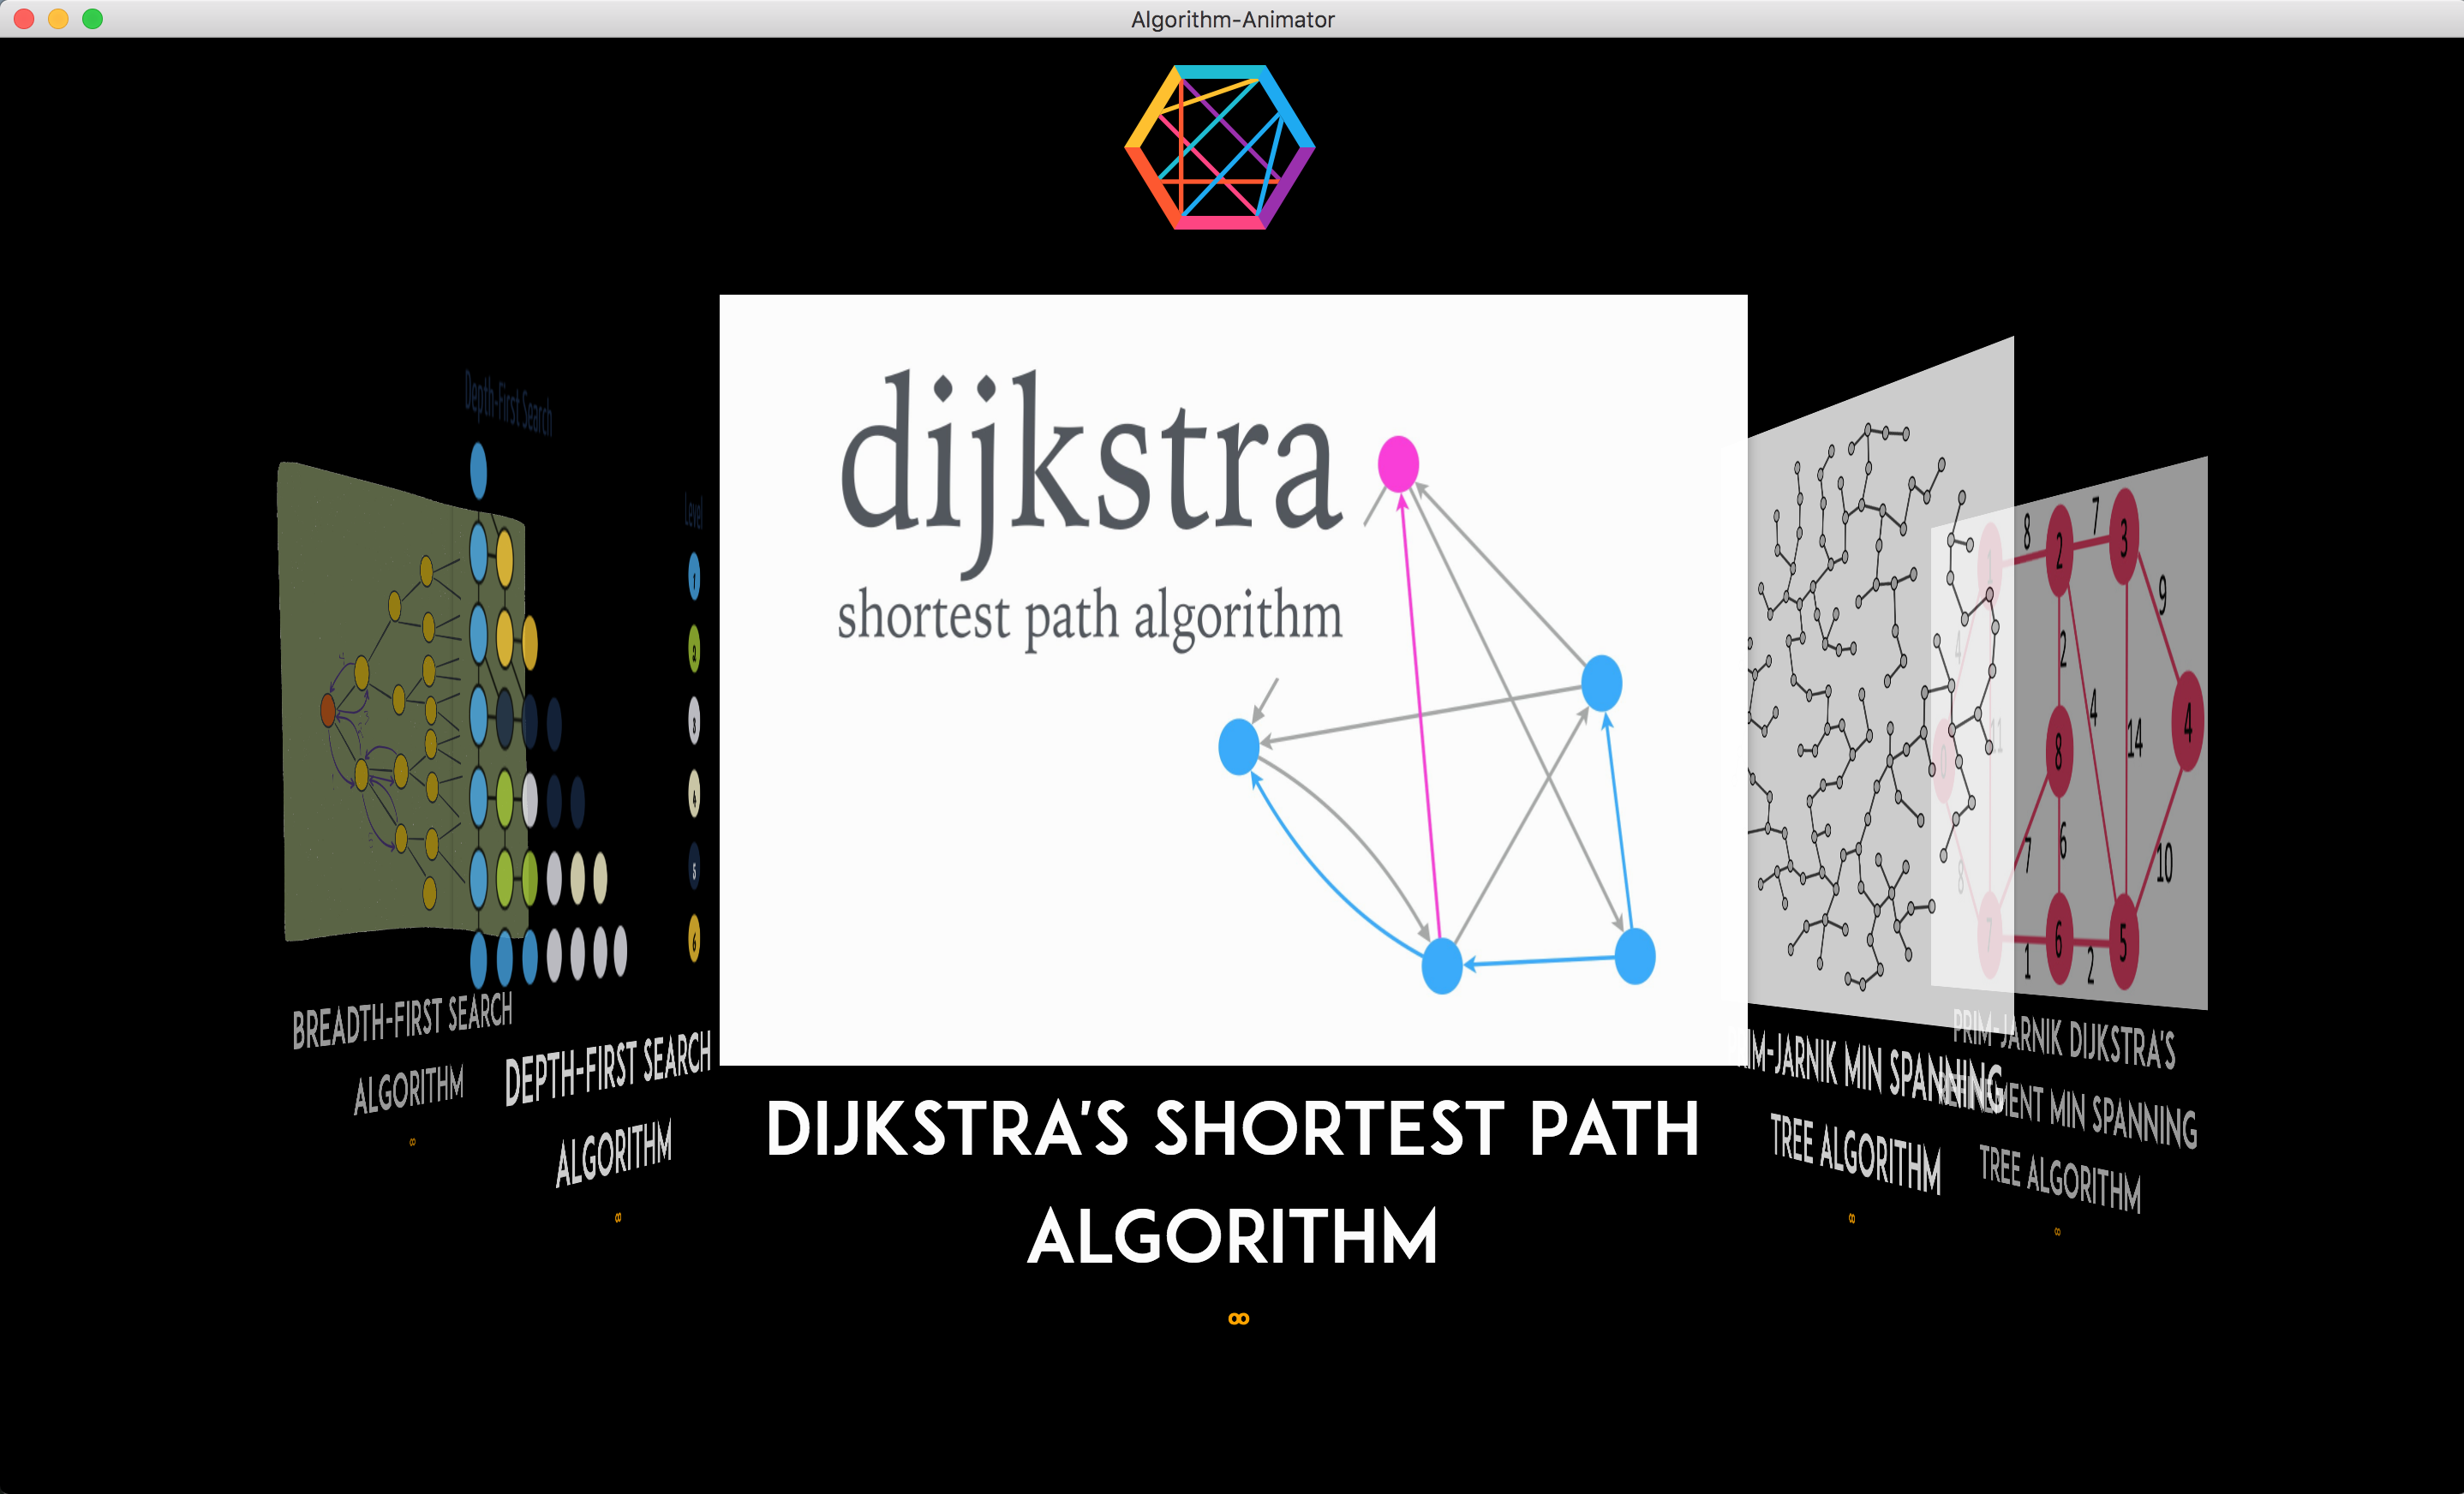
\includegraphics[scale=0.2]{landing-page}
\caption{Landing page in the application.}
\label{fig:landing-page}
\end{figure}

\pagebreak

Last but not least, we believe that having a modern and attractive webpage where users can download the application and get to
know some basic information is essential, thus we have created a custom website where we host the releases and users can simply
download and run Palgo with only a couple of clicks. This was a very nice feature voted for by many of our end users.
Figure~\ref{fig:palgo-website} shows a screenshot of the website.

\begin{figure}[!ht]
\centering
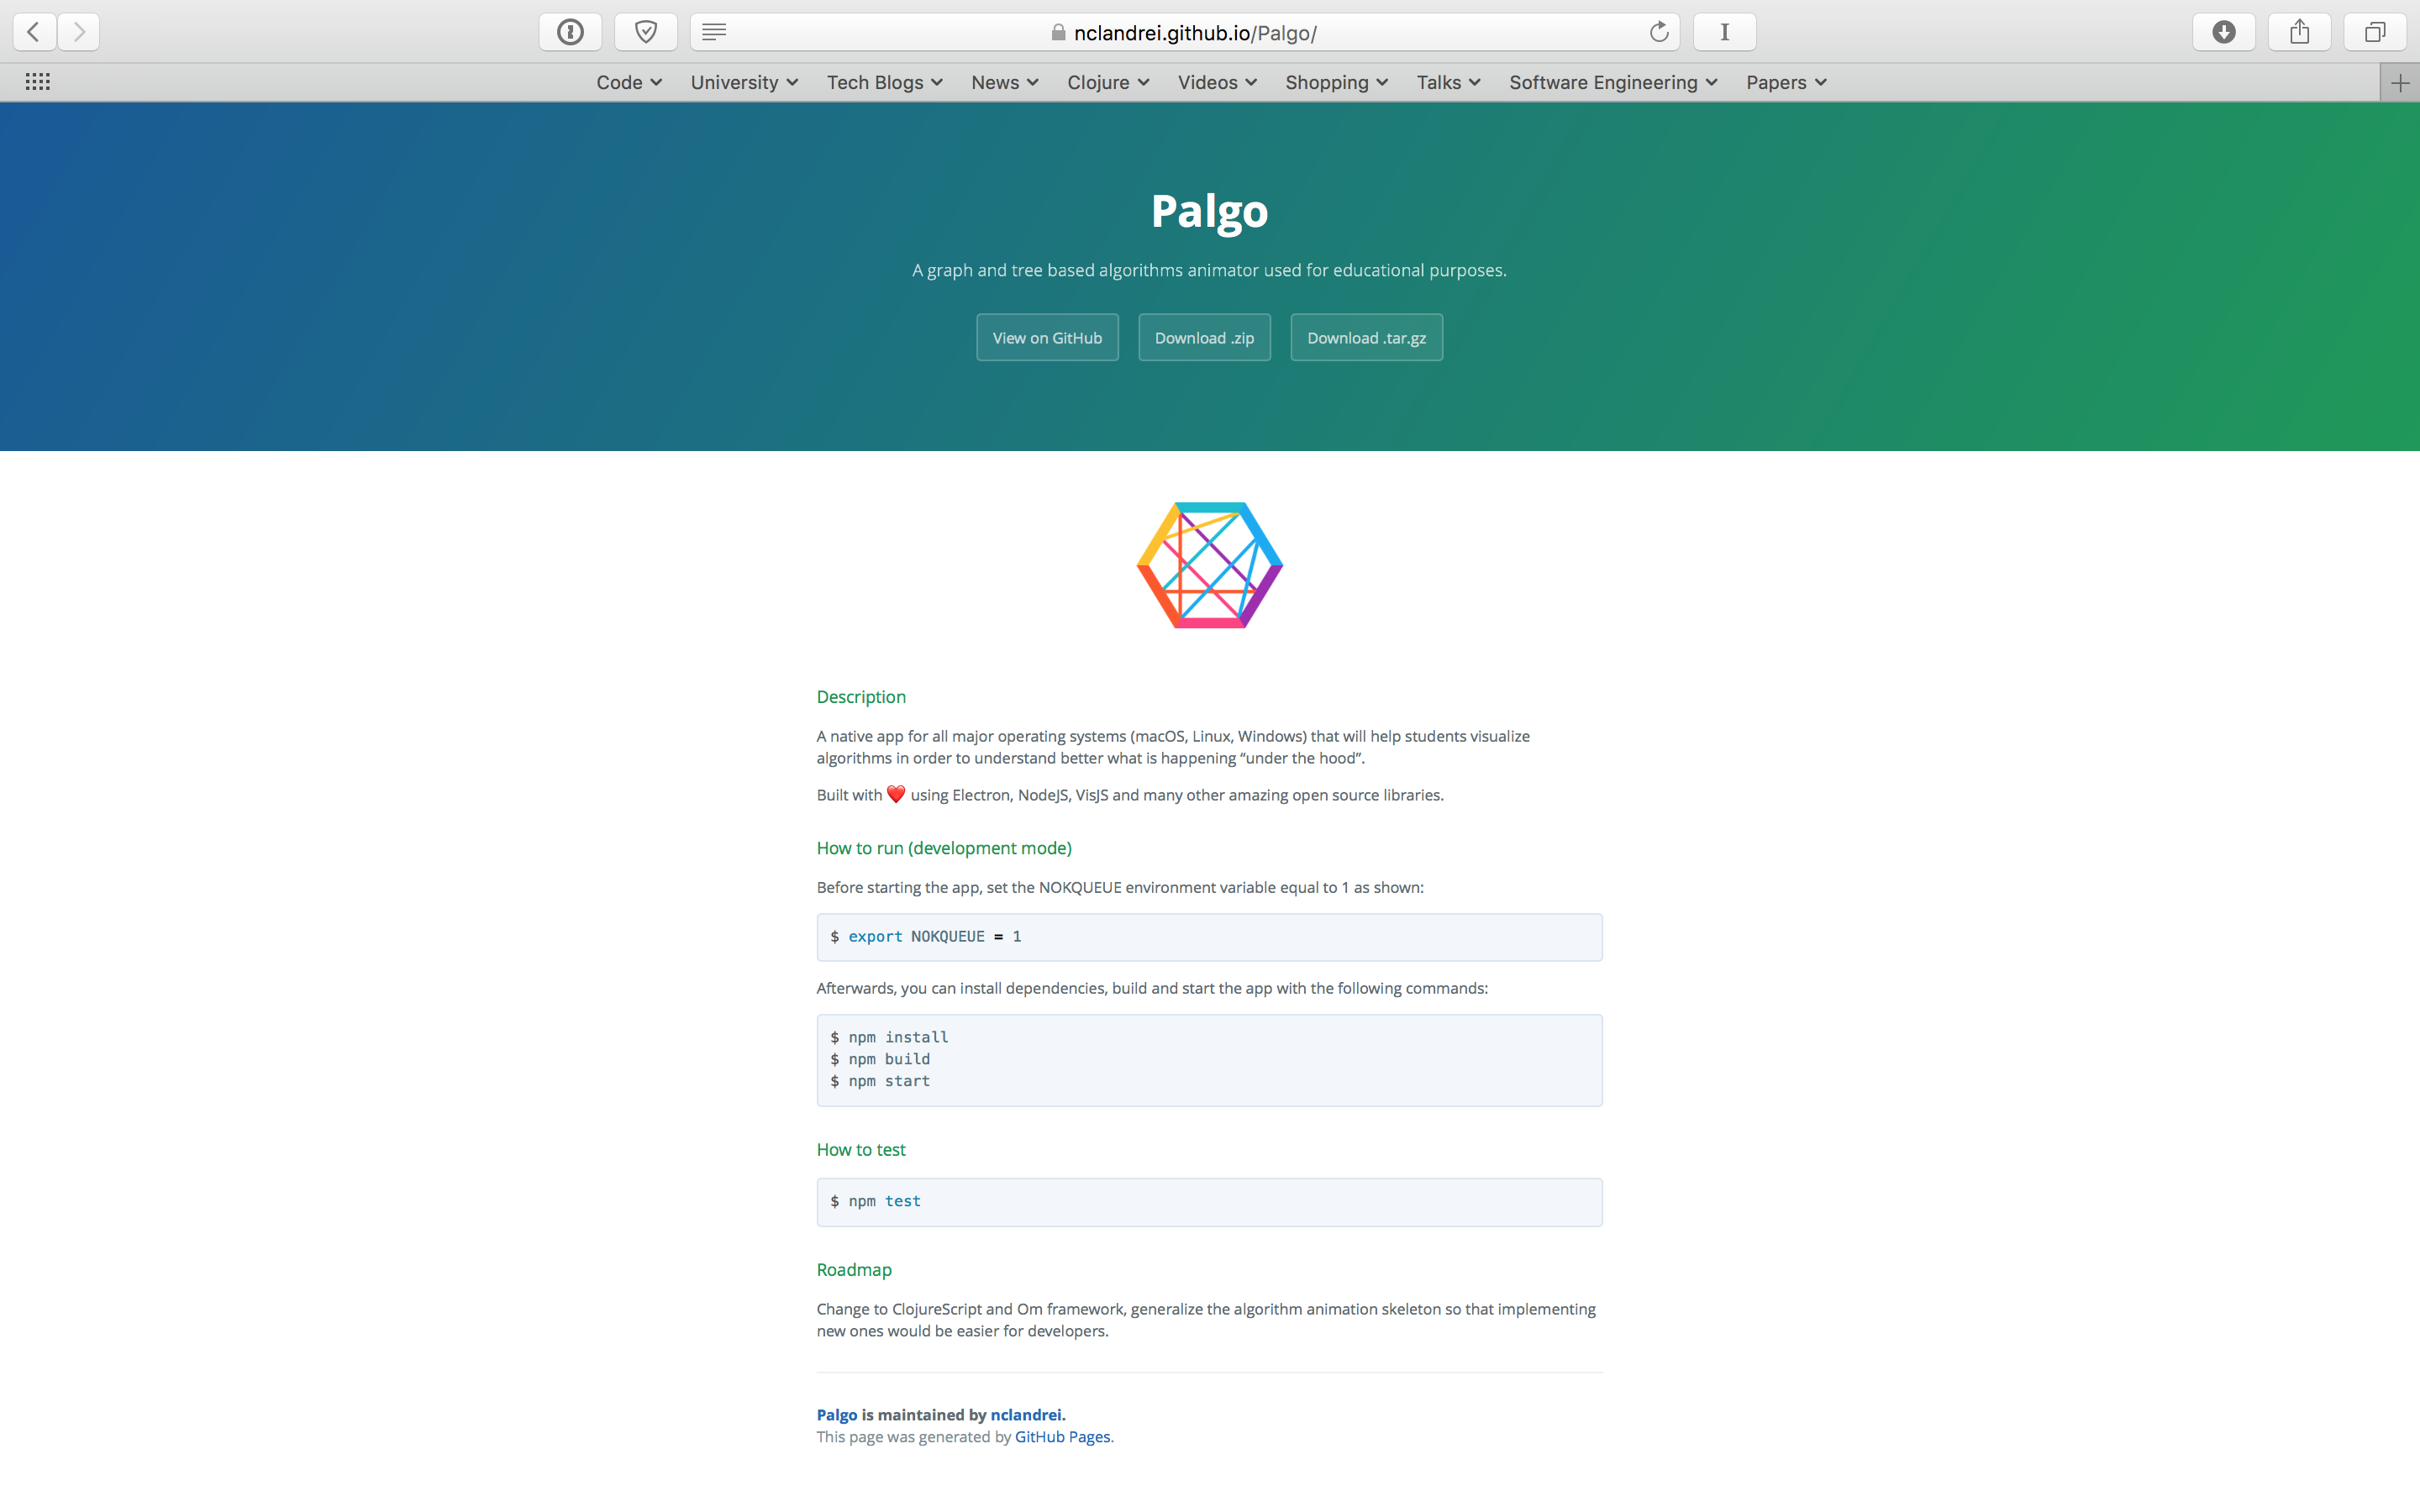
\includegraphics[scale=0.3]{palgo-website}
\caption{Palgo website hosted by GitHub.}
\label{fig:palgo-website}
\end{figure}

\section{Lessons Learned}

One of the most important lessons learned was that web development, even though it might sound easy, is not like that at all.
Because everything around us nowadays is web-based or it has something to do with it, there are a lot of technologies in
various sub-fields that help developers solve certain problems. As discussed in the previous sections, we have struggled
with many design decisions mainly because of the large palette of choices. Therefore, having to research and eventually
learn many of them so that argumented comparisons could be made regarding which one is better was time consuming.
However, once the developer possesses the basics, they can evolve and apply the fundamentals to learn any new
technology with ease.

Another lesson learned was that one needs to take very good care to not fall into the trap of ``premature optimization".
As we started the project back in first semester, I was very keen on implementing a large number of UI features such as
stylish buttons or attractive fade-ins when the window content changed. However, these early iterations were designed
for setting up the basics and implementing the algorithms, as well as animate them. Learning that optimizing prematurely
can lead to wasted effort, I have changed my approach and started prioritizing our user stories more effectively.

A third lesson I learned was that any JavaScript can fall in the ``callback hell". This is such a common pattern among
web developers that people created a website that specifically addresses this issue and gives advice on how to avoid
it~\cite{callback-hell}. I have also fell in this trap but with advice taken from the website mentioned previously, I
could easily refactor and follow the best practices promoted by industry leading developers.

Another vital aspect I have learned throughout this software process was the importance of code style in JavaScript. Even
though other programming languages promote a robust and consistent code style as well (e.g. Java, C), JavaScript is the
most popular technology used, and thus it has a very widespread reach. Therefore, many styling guides have been created so
that new developers would find code easier to read and, subsequently, to understand. The format I have used throughout
the whole project is a tool called Prettier~\cite{prettier} and the guide I used for reference is the one Airbnb have
open sourced on GitHub (it is now one of the most popular projects on the platform with almost 50,000
stars~\cite{airbnb-style-guide}). This will ensure that if the project gains contributors in the future, then their
accommodation period with the codebase will be smooth and fast.

Overall, I believe that this project was a real success and it was a great way to both learn new technologies as well as
learn how to research into previous work and apply the best software engineering practices. I think that without
following set rules, deadlines and good methodologies already proven successful in the industry, no project can ever
succeed.

%==============================================================================

\chapter{Testing}
\label{testing}

In this chapter we will discuss how we have tested our application to conform to the highest quality standards, how we used
CircleCI mixed with GitHub to do integration testing, as well as how we evaluated our application at the end of our
project and what results we achieved.

\section{Unit Testing}

Unit testing is a part of software testing in general that deals with individuals parts of the source code are tested
to check if they perform as expected.

JavaScript provides a large pool of frameworks to do unit testing. Even though they are quite different than what I was
used to (e.g. JUnit, Mockito, PyUnit) from university coursework and work experience, the fundamentals stay exactly the
same.

For our purposes we decided that MochaJS~\cite{mocha} was a great fit for the following reasons:

\begin{itemize}
  \item flexible and implemented with simplicity in mind;
  \item runs on node.js which was already one of our powering engines, thus the integration was straightforward;
  \item promotes a very descriptive documentation when writing tests because it uses the ``describe" and ``it" keyword
    which let the developer spot the failures easily;
  \item can integrate with various other frameworks such as should.js~\cite{shouldjs},
    better-assert~\cite{better-assert} and chai~\cite{chai}.
\end{itemize}

Through MochaJS we tested various animation and UI related components such as do the buttons work properly, are
algorithms correctly implemented in JS and give correct output or are codelines highlighted properly. However, in
order to test Electron itself and see if the native features behave as expected we hooked up another component:
Spectron~\cite{spectron}. It is a testing framework built by GitHub that uses ChromeDriver and WebDriverIO. 

As we discussed previously, using Mocha was very similar to what Java unit testing frameworks provide, but Spectron is
quite different. Listing~\ref{spectron-unit-test} is an example of one unit test written using Spectron.

\pagebreak

\begin{lstlisting}[language={Java}, label={spectron-unit-test}, caption={Spectron unit test which checks correct behaviour of the Electron
window.}]
var Application = require('spectron').Application
var assert = require('assert')

describe('application launch', function () {
  this.timeout(10000)

  beforeEach(function () {
    this.app = new Application({
      path: 'release-builds/macOS/Palgo'
    })
    return this.app.start()
  })
  afterEach(function () {
    if (this.app && this.app.isRunning()) {
      return this.app.stop()
    }
  })
  it('shows start screen', function () {
    return this.app.client.getWindowCount().then(function (count) {
      assert.equal(count, 1)
    })
  })
})
\end{lstlisting}

This is a simple unit test that starts the executable on macOS and checks if the window actually starts or not -
basically we are running a smoke test. Spectron was used mainly for checking if the application starts properly,
closes gracefully and also if a regular user workflow would break it.

Moreover, Spectron documentation promotes using MochaJS as the main testing framework to integrate with so our
accommodation with the two was natural.

\section{Integration Testing}

In terms of integration testing we have configured a circle.yml file which is required by CircleCI where we specified
that we want mocha to be our testing framework as well as the exact command how to run all the tests before merging
the code into master. The pipeline we have set up is as follows:

\begin{itemize}
  \item start running all the tests by running the mocha command (mocha was installed on the Linux server we have hooked
    up with CircleCI);
    \item if all tests passes, merge it into master, else (i.e. at least one test fails) abort merge and send an email specifying what tests failed and why;
  \item publish statistics on the CircleCI website and a small indicator next to the latest commit on the GitHub page
    showing the status of the build
    (i.e. green if passed, red if it did not).
\end{itemize}

This whole process ensured a smooth workflow and a continuous feedback on the status of our application and the
changes we were making.

\section{Prototype Evaluation}

The evaluation process was undergone together with 16 Level 4 Computer Science students at University of Glasgow. We
have asked them to complete a short form after using the application for approximately 20 minutes.

We provided the participants with a consent form where they were assured their whole input would be anonymous.
Also we have told them that they could stop at any time if they felt uncomfortable or any other reason during the
process.

The participants were split into 2 groups of 8 people each and the first group was told to use Palgo for 10 minutes while the
other group used Galant~\cite{galant}. We chose Galant because it is one of the most recently implemented algorithm
animators and it is also under active developmenton on GitHub~\cite{galant-github}.

The set of tasks they had to complete in both Palgo and Galant were:

\begin{itemize}
  \item start Palgo or Galant;
  \item select Depth-First Search algorithm;
  \item built a graph of 5 nodes, each being adjacent with at least another one;
  \item press start algorithm button;
  \item after it finished, press random button and observe the animations again;
  \item select Algorithms dropdown and go to Dijkstra's Shortest Path algorithm;
  \item repeat steps 3, 4 and 5;
  \item finally close the application through shortcut depending on the OS of choice or via the UI button;
\end{itemize}

After each group completed the tasks they switched with their colleagues and performed all the above steps for the other
animator. At the end of the evaluation trial we ran a questionaire (a Google form) regarding how
they found the two applications overall, what did they like/dislike and what they thought could be improved in
Palgo. 

We have used the best approaches in designing the questionnaire by getting expert advice from Dr. Oppengeim's book
``Questionnaire Design, Interviewing and Attitude Measurement"~\cite{questionnaire-design}. Thus, one of the techniques
we have used was that we have mixed possible
responses for multiple choice questions such that some begin with ``Much better" while others begin with ``Worst". Also, we have
kept the questionnaire short so that the users would not get exhausted after already completing 20 minutes of testing
the 2 applications. Overall, everyone seemed satisfied with our evaluation and no one experienced any problems throughout the process.

We have collected all results via Google Forms' built-in functionality and they will be presented in the next section.
The full questionnaire can be found in the Appendix.

\section{Results}

The results were astonishing as I did not believe that the application would receive such great impressions from the participants and
even desire to contribute to the project (see Appendix for complete results). The first question we selected was: ``How did you find using Palgo?".
Figure~\ref{fig:questionnaire-1} shows the feedback we received.

\begin{figure}[!ht]
    \centering
    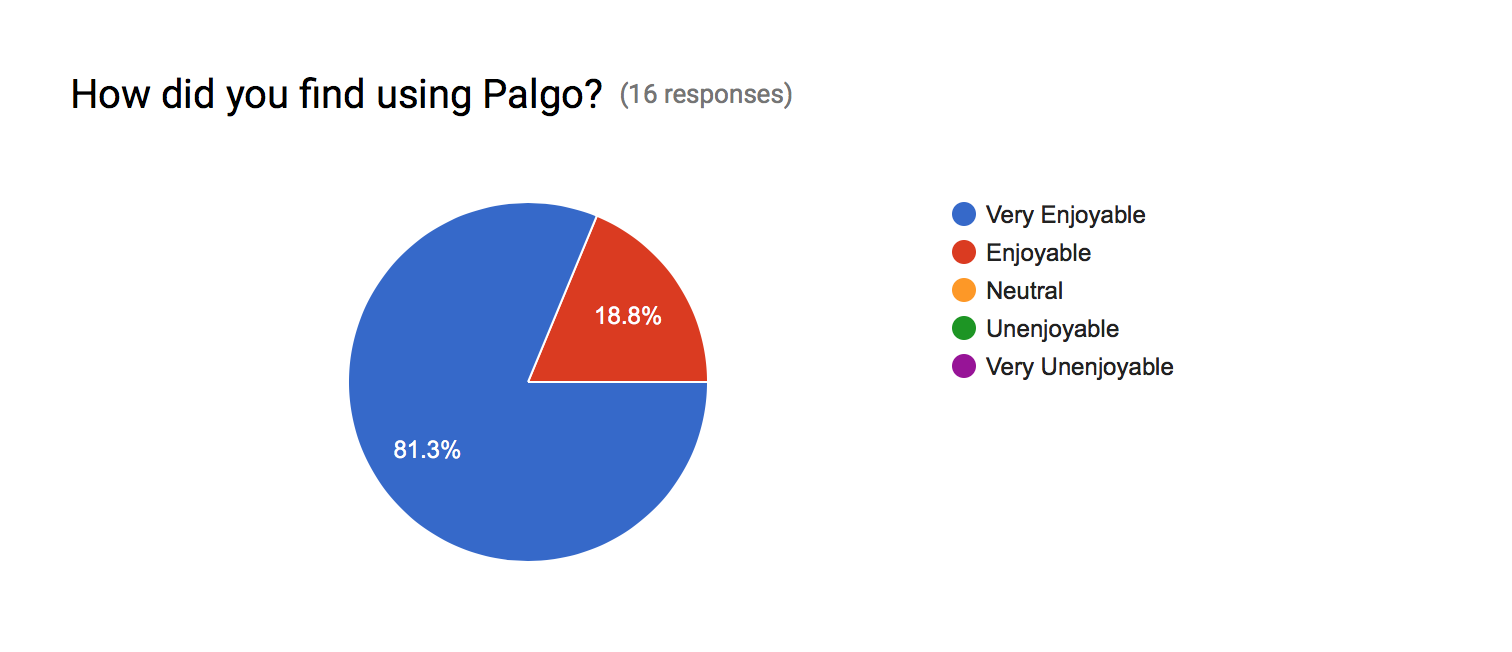
\includegraphics[scale=0.6]{questionnaire-1}
    \caption{Feedback on question: How did you find using Palgo?}
    \label{fig:questionnaire-1}
\end{figure}

As it can be observed, all responses were either ``Enjoyable" or ``Very Enjoyable". This was an
important achievement for our project because it showed how focus on simplicity, efficiency and state-of-the-art
software engineering practices
can produce an application of high quality that would indeed be enjoyed by end users. Even though most of the questions
were related specifically to our implementation of the animator, we also introduced Galant as a point of reference and
asked our participants to compare the two. The results were even more surprising as depicted in Figure~\ref{fig:questionnaire-2}.

\begin{figure}[!ht]
    \centering
    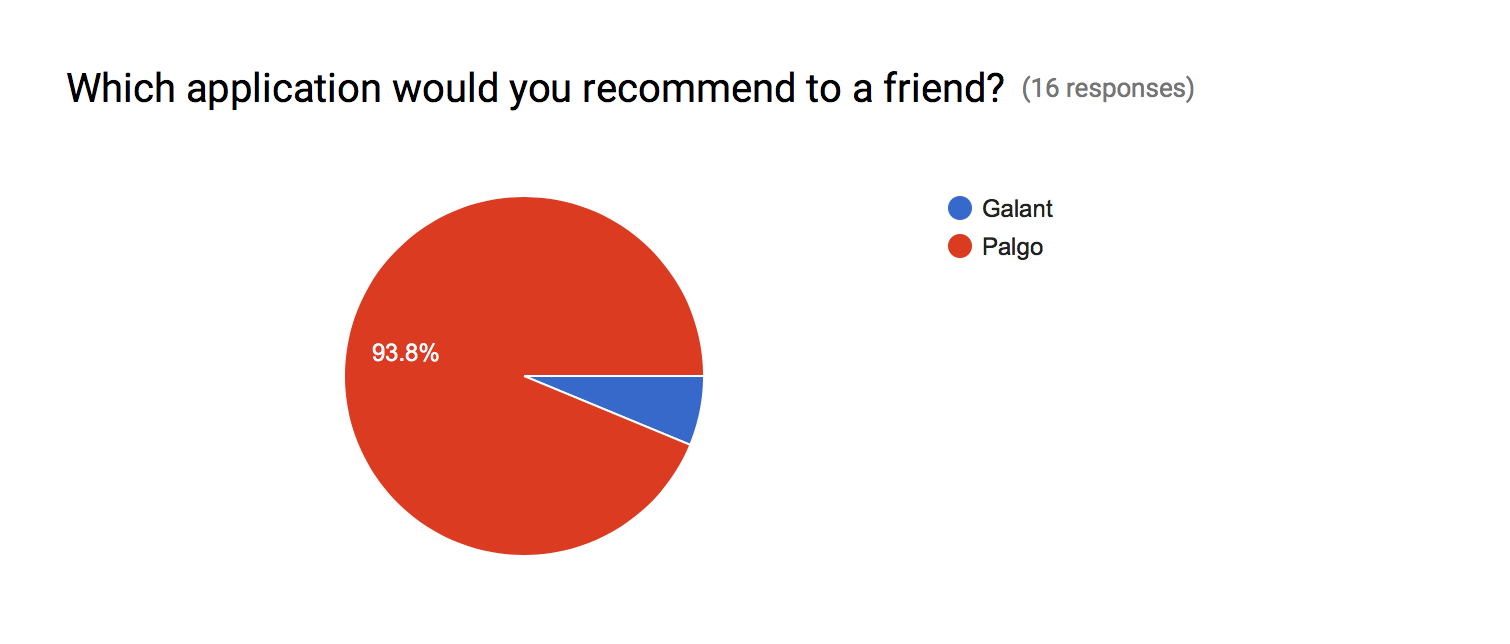
\includegraphics[scale=0.6]{questionnaire-2}
    \caption{Feedback on question: Which application would you recommend to a friend?}
    \label{fig:questionnaire-2}
\end{figure}

15 out of 16 participants preferred Palgo over Galant even though the latter is a tool being actively under
development for almost 3 years.

Summing up our findings, we can happily say that the evaluation proved that our project has been a real success with an
actual potential of becoming developed by more than one contributor and used by many more.

%==============================================================================

\chapter{Conclusions}
\label{conclusions}

In this chapter we will wrap up this document with why we want to keep the application open source and try to promote it
so that there would be more contributors, future work and the roadmap we have in mind, some final thoughts and, last but
not least, acknowledgements.

\section{Open Source}

Open Source is one of the main engines behind the whole software world. Virtually every developer uses open source projects in
their day-to-day workflow and many of them contribute to this amazing community. Without Electron, Vis.JS, MochaJS
and many other technologies, Palgo would not exist today so we could not be more grateful to the great community
that produced all this high quality software.

Therefore, we would definitely proceed with hosting the project on GitHub and start to promote it on various platforms
(e.g.\ social media, email within university students) so that more people would use it and, even better, contribute to
improving it.

\section{Project Roadmap}

Future work is vital for the project as the application is yet to be fully finished. We have divided these plans into
the following categories.

\begin{itemize}
  \item Change the JavaScript code into ClojureScript~\cite{clojurescript} - this is because ClojureScript is an
    amazing functional programming language which puts emphasis on immutability and a pure functional style; we
    believe that this would benefit us in the long term through a more concise and simple approach to implementing new
    algorithms.
  \item Modify the codebase to include React~\cite{react} - React is a technology built by Facebook which basically adds a
    new virtual DOM (hooks it at some point on the actual DOM) and focuses on reusability of components. Moreover, it
    uses JSX~\cite{jsx} which is a mixture of JavaScript and HTML5, thus you can create your whole page through pure
    JS;.
  \item As previously mentioned, we will keep the project open source on GitHub and try to add more collaborators so
    that people can contribute to Palgo and add in both new features and algorithms to be animated.
  \item Even though we have mentioned in Chapter~\ref{background} about related work to more complex algorithms (e.g.
    parallel computing) and how there is virtually no animator that can show such algorithms, we will try to explore
    the opportunity and see if we can actually add them to Palgo in the future.
  \item I have already began negotiations with some Computer Science teachers from home (Romania) to consider adding
    Palgo as a teaching tool in their classes; if there will be people who agree to the idea we will add Romanian
    localization and maintain both languages from that point onwards.
  \item Having discussed with Dr. Norman about possible outcomes for Palgo we have also talked about the idea of
    proposing the application as a starting point for students that will take the ``Algorithm Animator" project next
    year; this way we can make sure we will have collaborators to help us continue our work.
\end{itemize}

Because I have grown to be attached to the application the last point that the reader needs to get from this
section is that the project will definitely not be thrown away and we will keep developing it and make it even a
better tool to help people understand algorithms easily while also having fun.

\section{Final Thoughts}

I believe that the Level 4 Project was an amazing opportunity to not only learn new technologies, but also apply
software engineering practices in real
world. I have learned how to use many tools that I did not know about beforehand such as MochaJS or Electron. Also, I
have researched and found out best approaches to write clean and simple code that would be easy to maintain and scale. 

Moreover, applying what we have learned both last year in Professional Software Development and this year in Advanced Software Engineering Practices was both fun and hard to master.
Theoretically speaking, nothing seems hard, but when you put it in practice you realize you did not know that much about
the techniques. This was a valuable lesson I was given during this project.

In the end, I do believe that Palgo will not ``die" because I will begin to promote it and continue to develop it even
further. Also, after discussions with Dr. Norman, the project will be included as a resource on the Moodle page for
Algorithmics I students, thus its reach will expand from that moment onwards.

\section{Acknowledgements}

To begin with, I would like to thank Dr. Gethin Norman who was not only my supervisor but also a great team member. He
has helped me with everything throughout the whole year and without his input and help Palgo would not exist today.

Furthermore, I'd like to say thank you to every student who has participated during ``customer'' meetings during the year
as well as to all the people who helped us with the evaluation at the end of the software process.

Last but not least, I would like to thank every developer that has contributed even one source code line to the amazing open source projects
we have used throughout our algorithm animator. Without them Palgo would not look and perform the way it does in
the final release.

%%%%%%%%%%%%%%%%
%              %
%  APPENDICES  %
%              %
%%%%%%%%%%%%%%%%

\begin{appendices}
  \chapter{Evaluation Questionnaire}
  \label{evaluation-questionnaire}
  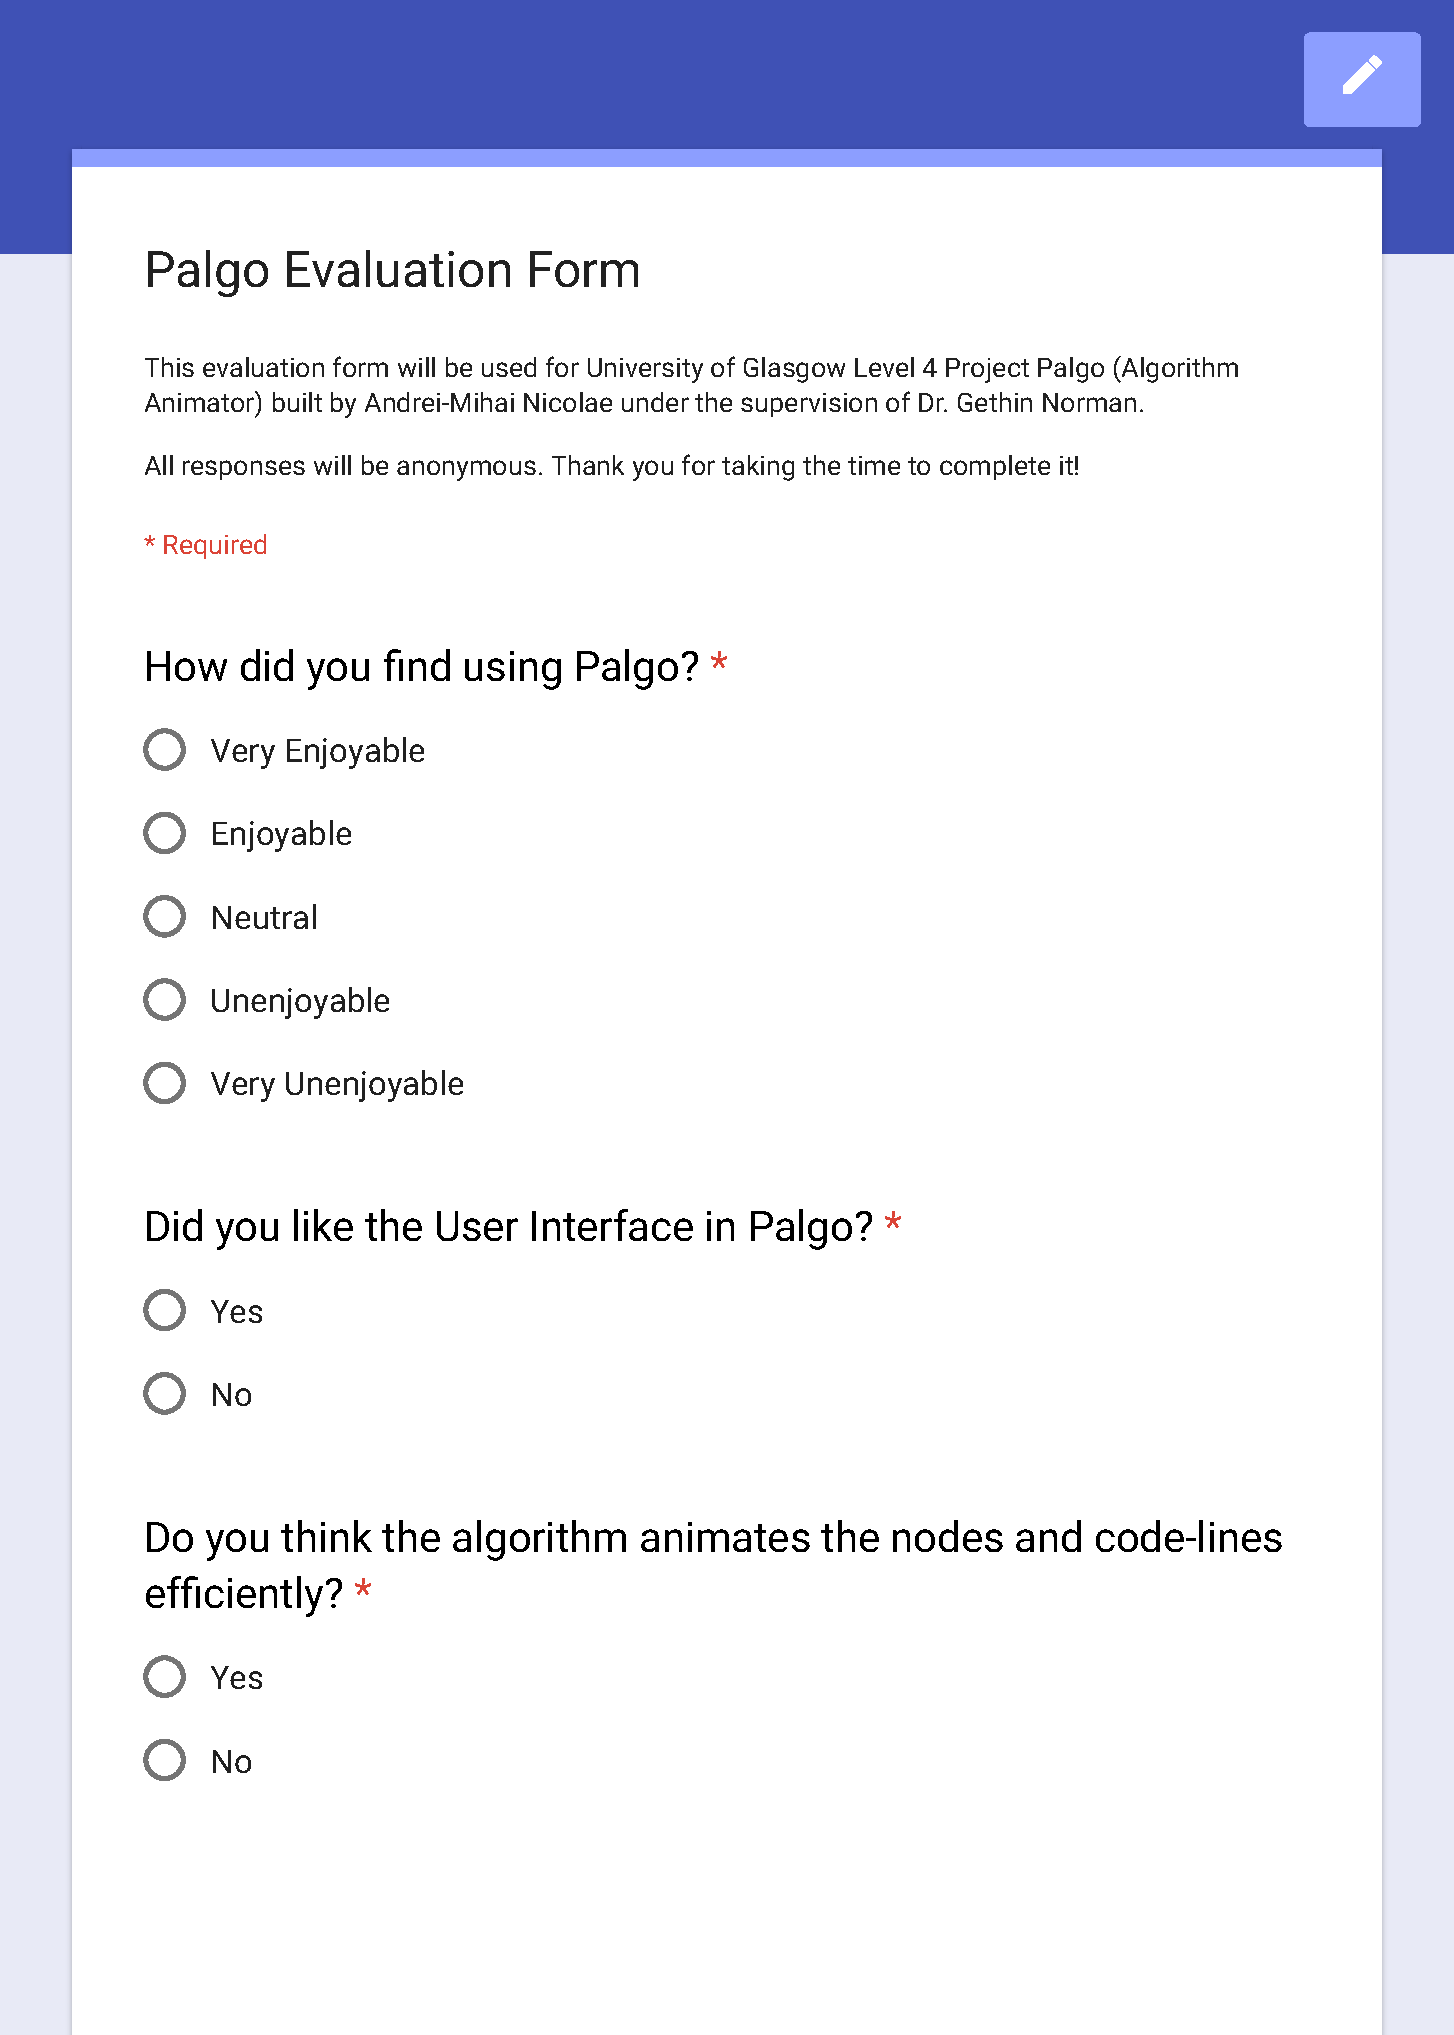
\includepdf[pages=-, pagecommand={}, width=\textwidth]{palgo-evaluation-form.pdf}
  \chapter{Evaluation Feedback}
  \label{evaluation-feedback}
  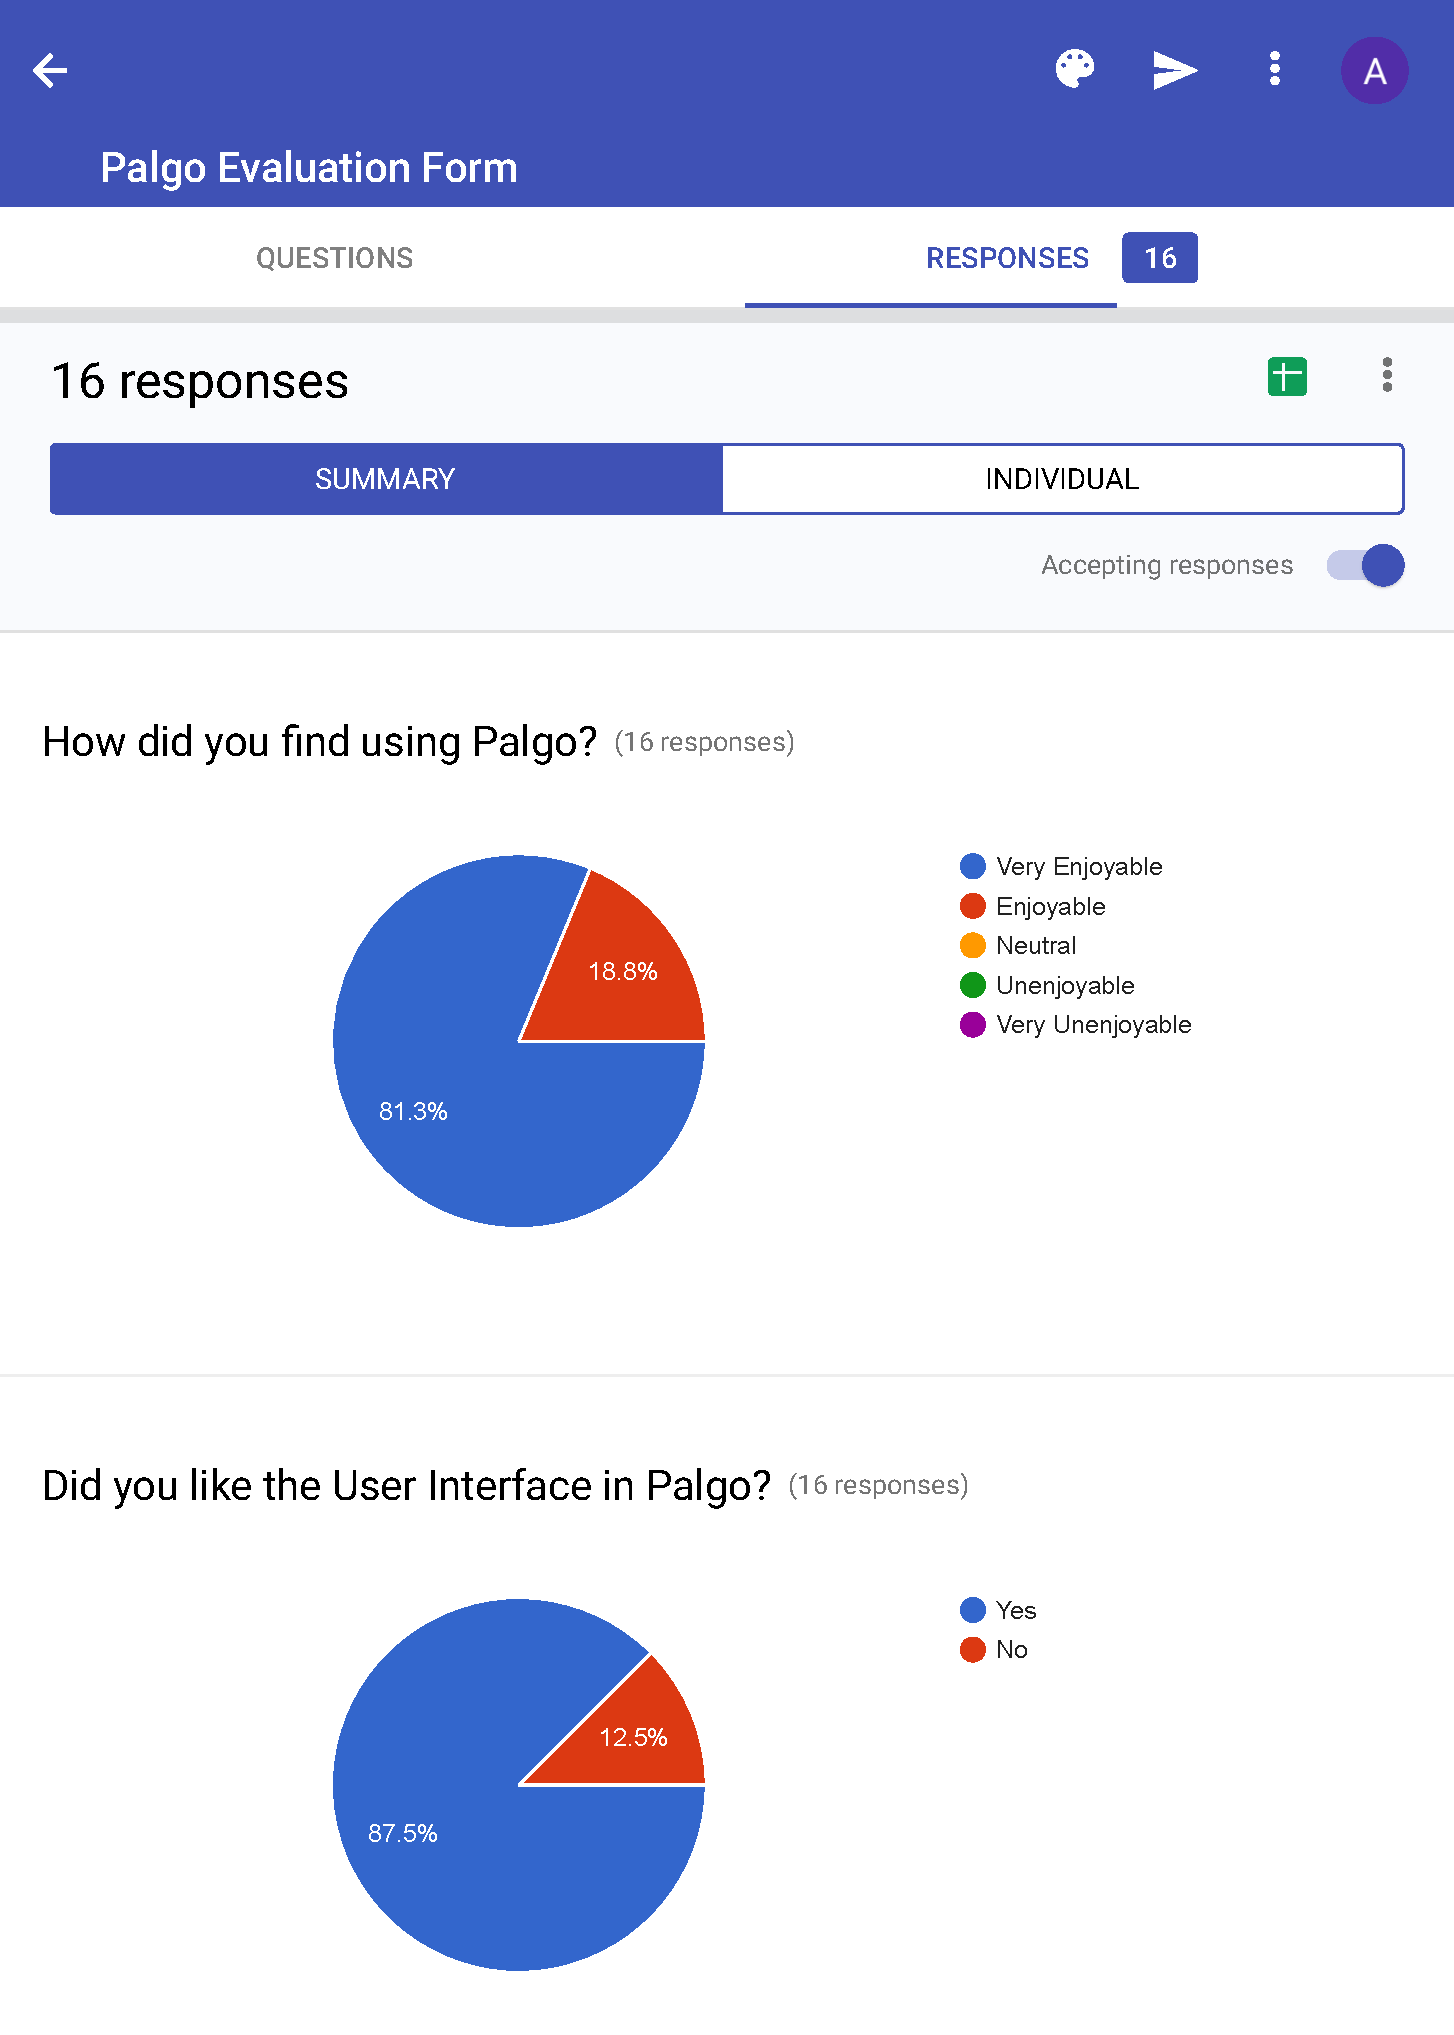
\includepdf[pages=-, pagecommand={}, width=\textwidth]{palgo-evaluation-responses.pdf}
\end{appendices}

%%%%%%%%%%%%%%%%%%%%
%   BIBLIOGRAPHY   %
%%%%%%%%%%%%%%%%%%%%

\bibliographystyle{plain}
\bibliography{l4proj}
\end{document}
